
\documentclass[10pt]{article}

\usepackage{fullpage}
\usepackage[utf8]{inputenc}
\usepackage[T1]{fontenc}

\usepackage{makecell}
\usepackage{enumitem}
\usepackage{hyperref}
\usepackage{amsmath}
\usepackage{pdflscape}
\usepackage{wasysym}
\usepackage{longtable}
\usepackage[style=ieee, url=true]{biblatex}
\addbibresource{benchmarks.bib} 
\usepackage{caption}
\usepackage{url}
\usepackage{graphicx}
\graphicspath{{images/}}


\usepackage{textcomp}
\usepackage{amssymb}
\usepackage{eurosym} 
\usepackage{pifont} 


\DeclareUnicodeCharacter{0394}{\Delta}


\tolerance=10000
\hfuzz=100pt
\emergencystretch=3em
\hbadness=10000

\setlength{\parindent}{0pt}

\begin{document}
\sloppy
\author{Gregor von Laszewski,
          Reece Shiraishi, 
          Anjay Krishnan, 
          Nhan Tran, \\
          Benjamin Hawks, and 
          Geoffrey C. Fox}

\date{\today}
\title{MLCommons Science Working Group AI Benchmarks Collection}
\maketitle

\begin {abstract}
This document provides an overview of various benchmarks, including their descriptions, URLs, domains, focus areas, keywords, task types, AI capabilities measured, metrics, models, and notes. Each benchmark
\end{abstract}

\vfill 

{\centering \bfseries Citation \par}

\begin{quote}
\begin{verbatim}
@misc{benchmark-collection,
  title={MLCommons Science Working Group AI Benchmarks Collection}
  author={Gregor von Laszewski and 
          Reece Shiraishi and 
          Anjay Krishnan and 
          Nhan Tran and 
          Benjamin Hawks and 
          Geoffrey C. Fox}
  url={https://mlcommons-science.github.io/benchmark/benchmarks.pdf}
  howpublished={Github},
  year={2025}
  month=jul
}
\end{verbatim}
\end{quote}
\clearpage
\tableofcontents
\clearpage


\section{Benchmark Overview Table}


\begin{landscape}
{\footnotesize
\begin{longtable}{|p{0.13\textwidth}|p{0.11\textwidth}|p{0.09\textwidth}|p{0.09\textwidth}|p{0.11\textwidth}|p{0.13\textwidth}|p{0.13\textwidth}|p{0.09\textwidth}|p{0.09\textwidth}|p{0.04\textwidth}|}
\hline
\textbf{Ratings} & \textbf{Name} & \textbf{Domain} & \textbf{Focus} & \textbf{Keywords} & \textbf{Task Types} & \textbf{AI Capability} & \textbf{Metrics} & \textbf{Models} & \textbf{Citation}  \\ \hline
\endfirsthead
\hline
\textbf{Ratings} & \textbf{Name} & \textbf{Domain} & \textbf{Focus} & \textbf{Keywords} & \textbf{Task Types} & \textbf{AI Capability} & \textbf{Metrics} & \textbf{Models} & \textbf{Citation}  \\ \hline
\endhead
\hline
\multicolumn{10}{r}{Continued on next page} \\
\endfoot
\hline
\endlastfoot
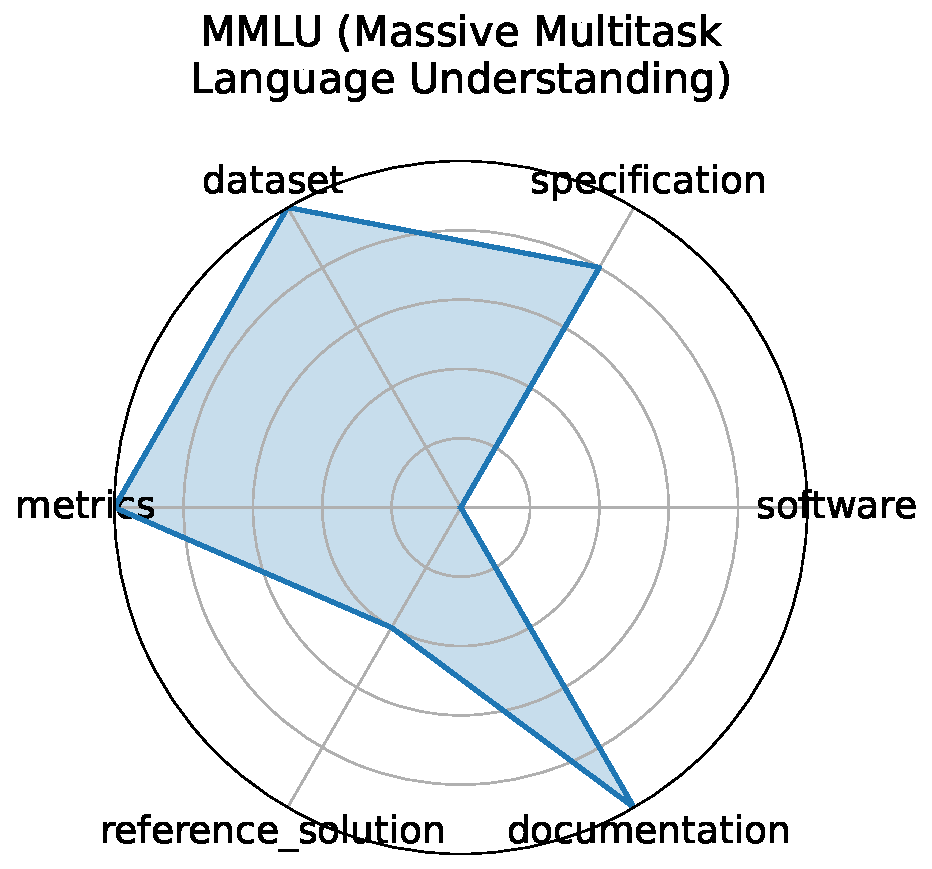
\includegraphics[width=0.15\textwidth]{mmlu_massive_multitask_language_understanding_radar.pdf} & MMLU (Massive Multitask Language Understanding) & Multidomain & Academic knowledge and reasoning across 57 subjects & multitask, multiple-choice, zero-shot, few-shot, knowledge probing & Multiple choice & General reasoning, subject-matter understanding & Accuracy & GPT-4o, Gemini 1.5 Pro, o1, DeepSeek-R1 & \cite{hendrycks2021measuring}\href{https://paperswithcode.com/dataset/mmlu}{$\Rightarrow$} \\ \hline
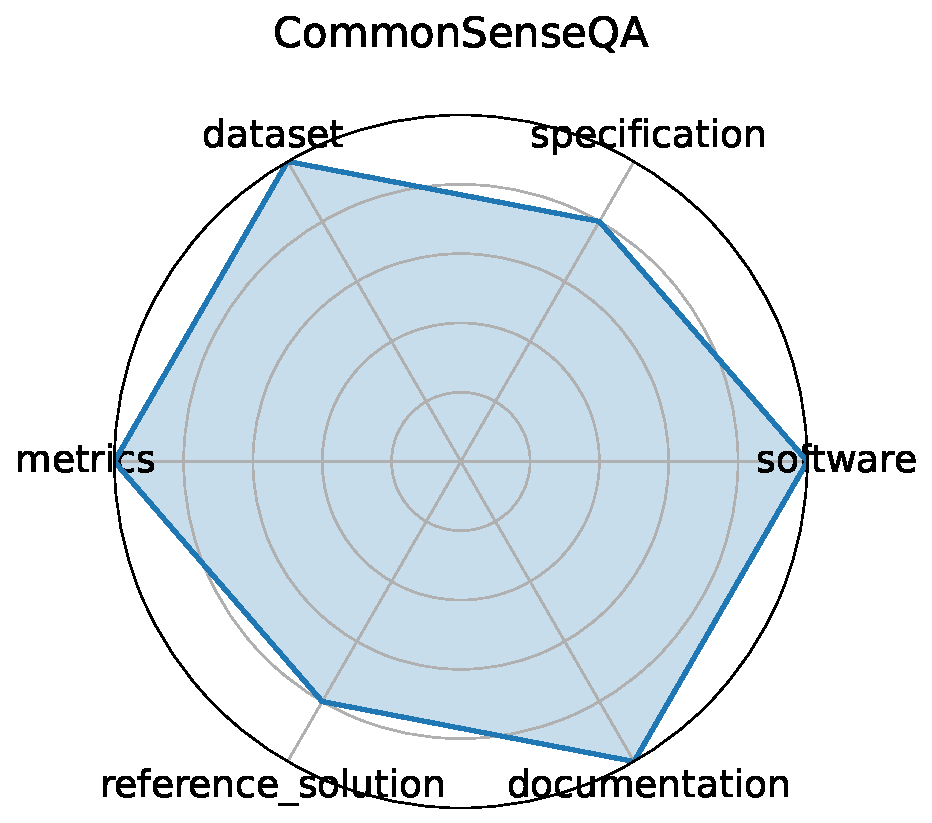
\includegraphics[width=0.15\textwidth]{commonsenseqa_radar.pdf} & CommonSenseQA & NLP; Commonsense & Commonsense question answering & ConceptNet, multiple-choice, adversarial & Multiple choice & Commonsense reasoning and knowledge integration & Accuracy & BERT-large, RoBERTa, GPT-3 & \cite{talmor2019commonsenseqaquestionansweringchallenge}\href{https://paperswithcode.com/paper/commonsenseqa-a-question-answering-challenge}{$\Rightarrow$} \\ \hline
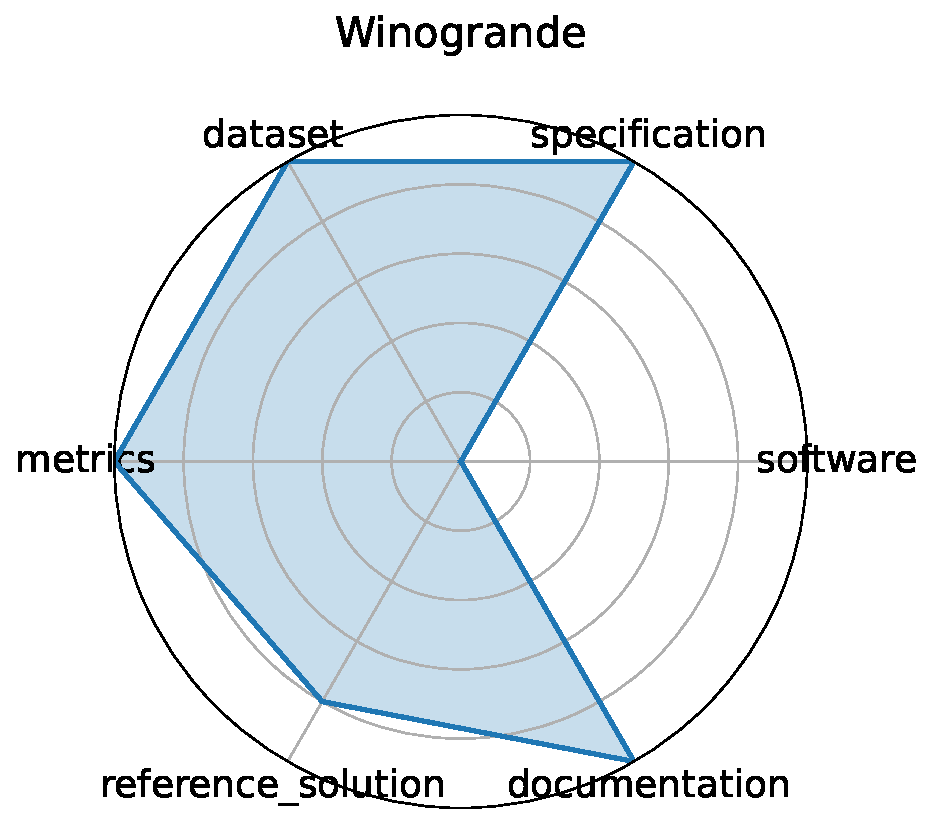
\includegraphics[width=0.15\textwidth]{winogrande_radar.pdf} & Winogrande & NLP; Commonsense & Winograd Schema-style pronoun resolution & adversarial, pronoun resolution & Pronoun resolution & Robust commonsense reasoning & Accuracy, AUC & RoBERTa, BERT, GPT-2 & \cite{sakaguchi2019winograndeadversarialwinogradschema}\href{https://leaderboard.allenai.org/winogrande/submissions/public}{$\Rightarrow$} \\ \hline
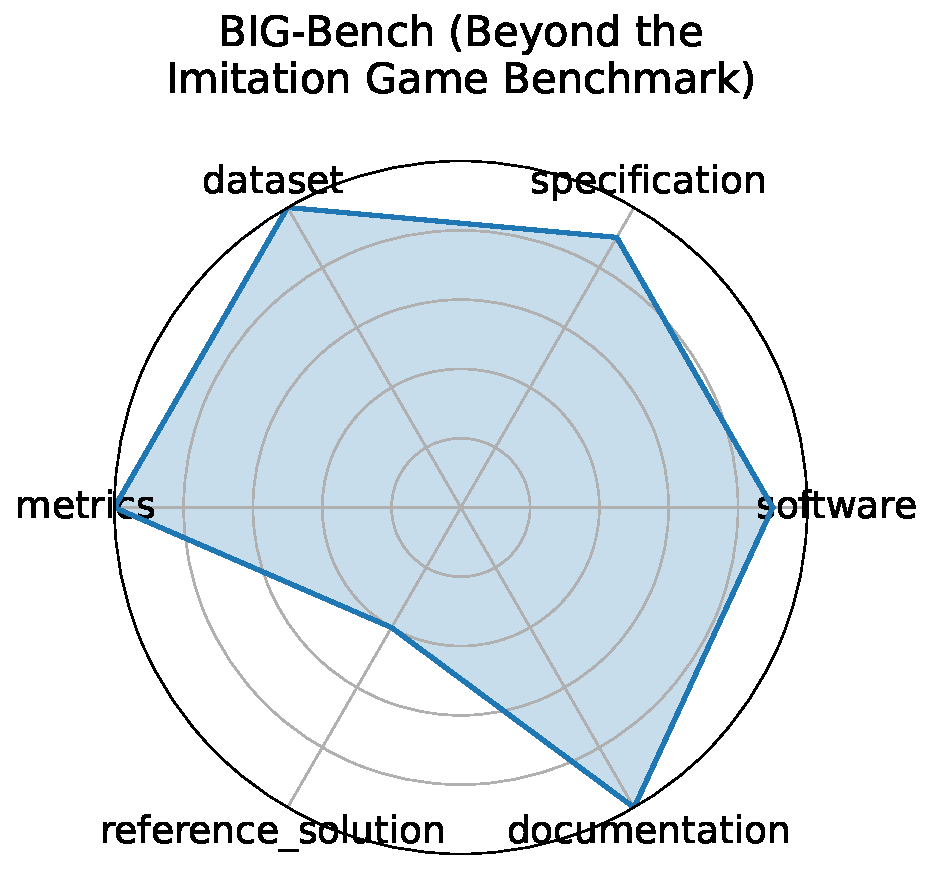
\includegraphics[width=0.15\textwidth]{big-bench_beyond_the_imitation_game_benchmark_radar.pdf} & BIG-Bench (Beyond the Imitation Game Benchmark) & NLP; AI Evaluation & Diverse reasoning and generalization tasks & few-shot, multi-task, bias analysis & Few-shot evaluation, Multi-task evaluation & Reasoning and generalization across diverse tasks & Accuracy, Task-specific metrics & GPT-3, Dense Transformers, Sparse Transformers & \cite{srivastava2023imitationgamequantifyingextrapolating}\href{https://github.com/google/BIG-bench}{$\Rightarrow$} \\ \hline
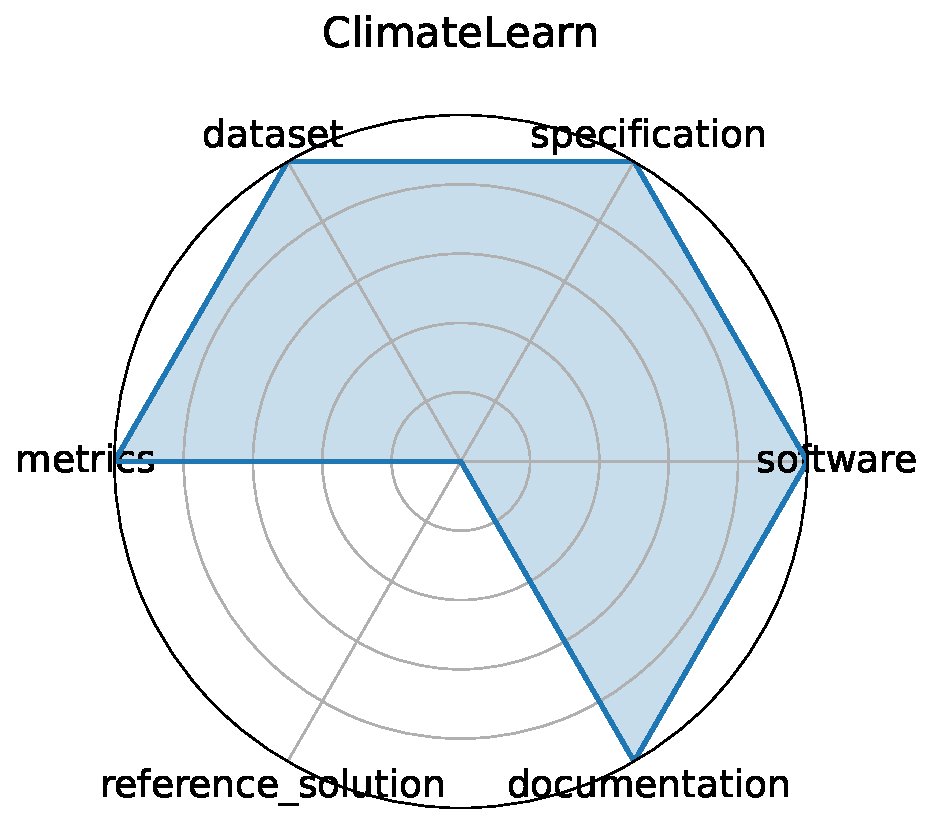
\includegraphics[width=0.15\textwidth]{climatelearn_radar.pdf} & ClimateLearn & Climate Science; Forecasting & ML for weather and climate modeling & medium-range forecasting, ERA5, data-driven & Forecasting & Global weather prediction (3-5 days) & RMSE, Anomaly correlation & CNN baselines, ResNet variants & \cite{nguyen2023climatelearnbenchmarkingmachinelearning}\href{https://arxiv.org/abs/2307.01909}{$\Rightarrow$} \\ \hline
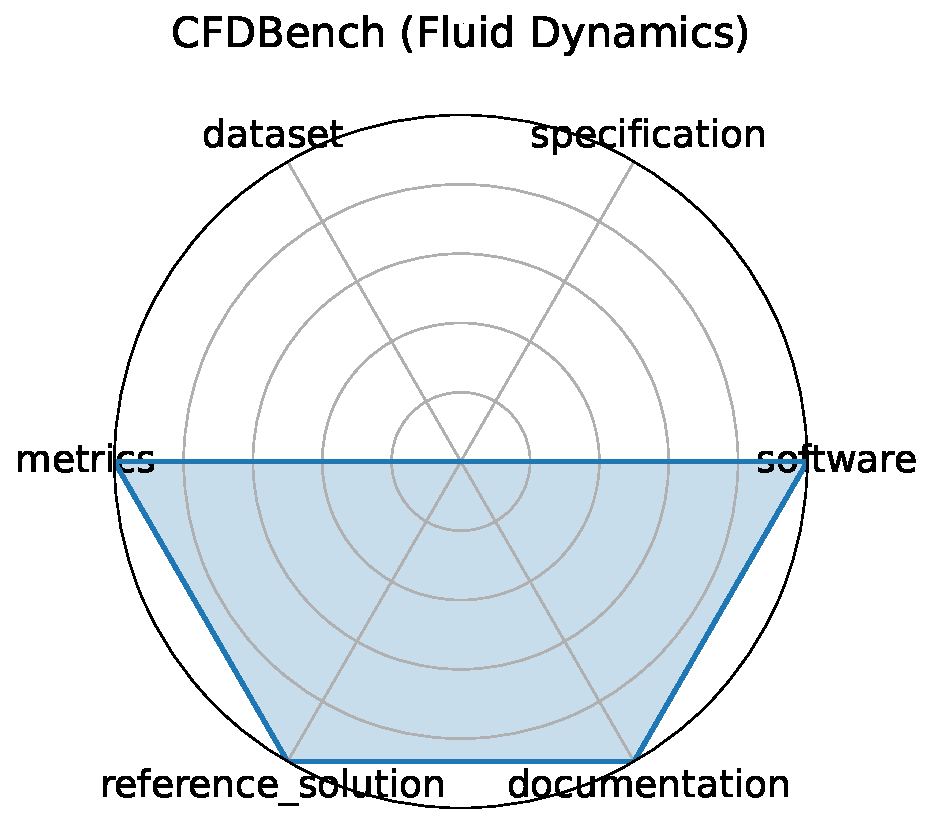
\includegraphics[width=0.15\textwidth]{cfdbench_fluid_dynamics_radar.pdf} & CFDBench (Fluid Dynamics) & Fluid Dynamics; Scientific ML & Neural operator surrogate modeling & neural operators, CFD, FNO, DeepONet & Surrogate modeling & Generalization of neural operators for PDEs & L2 error, MAE & FNO, DeepONet, U-Net & \cite{luo2024cfdbenchlargescalebenchmarkmachine}\href{https://arxiv.org/abs/2310.05963}{$\Rightarrow$} \\ \hline
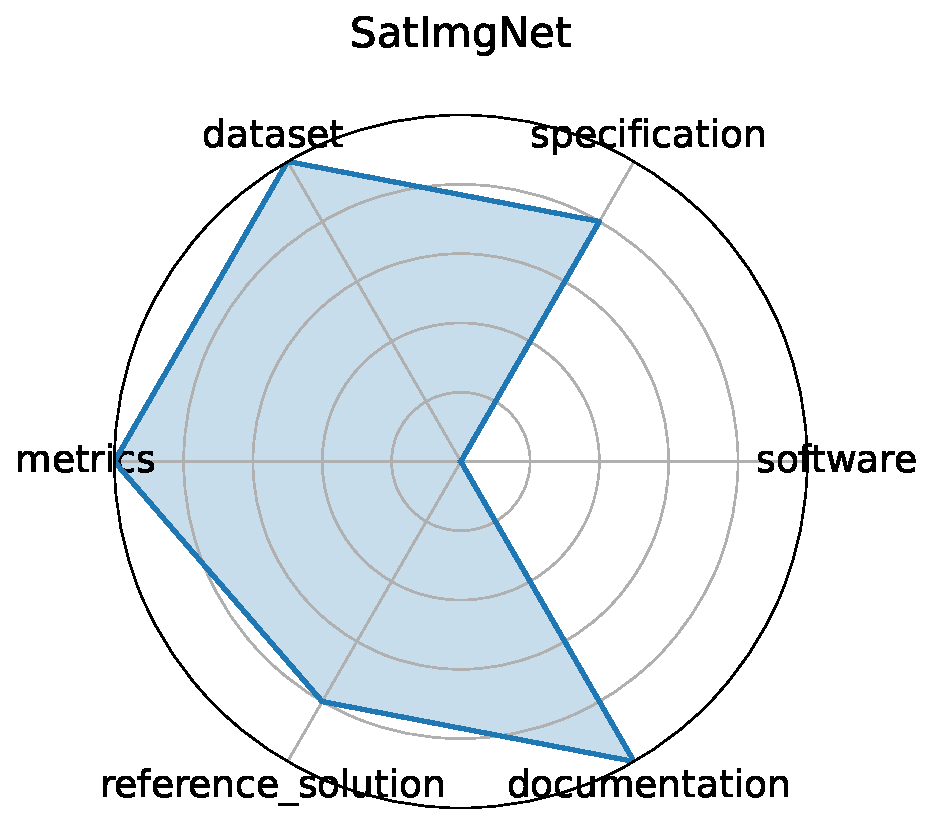
\includegraphics[width=0.15\textwidth]{satimgnet_radar.pdf} & SatImgNet & Remote Sensing & Satellite imagery classification & land-use, zero-shot, multi-task & Image classification & Zero-shot land-use classification & Accuracy & CLIP, BLIP, ALBEF & \cite{roberts2023satin}\href{https://huggingface.co/datasets/saral-ai/satimagnet}{$\Rightarrow$} \\ \hline
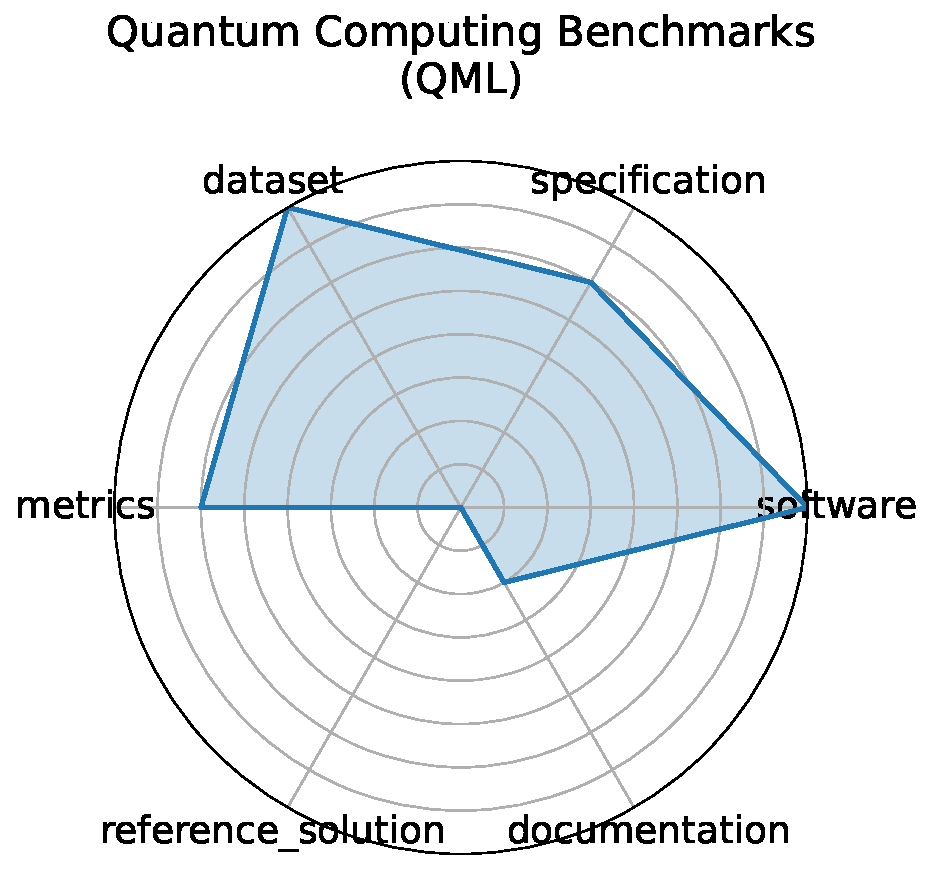
\includegraphics[width=0.15\textwidth]{quantum_computing_benchmarks_qml_radar.pdf} & Quantum Computing Benchmarks (QML) & Quantum Computing & Quantum algorithm performance evaluation & quantum circuits, state preparation, error correction & Circuit benchmarking, State classification & Quantum algorithm performance and fidelity & Fidelity, Success probability & IBM Q, IonQ, AQT@LBNL & \cite{kiwit2023}\href{https://github.com/XanaduAI/qml-benchmarks}{$\Rightarrow$} \\ \hline
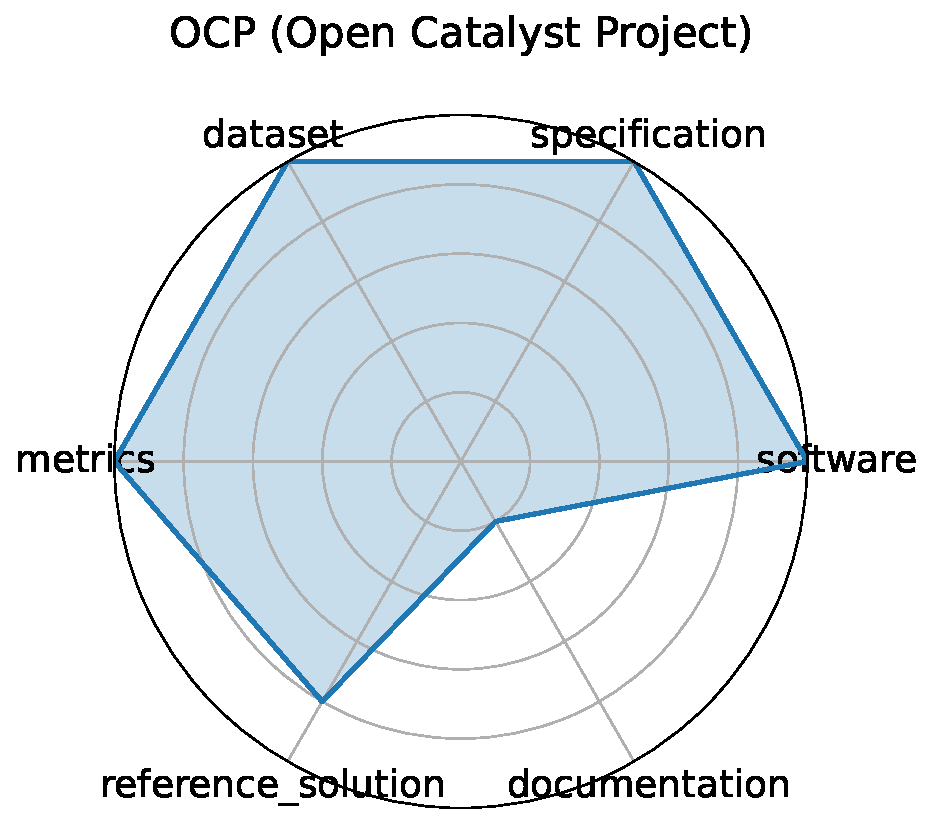
\includegraphics[width=0.15\textwidth]{ocp_open_catalyst_project_radar.pdf} & OCP (Open Catalyst Project) & Chemistry; Materials Science & Catalyst adsorption energy prediction & DFT relaxations, adsorption energy, graph neural networks & Energy prediction, Force prediction & Prediction of adsorption energies and forces & MAE (energy), MAE (force) & CGCNN, SchNet, DimeNet++, GemNet-OC & \cite{chanussot2021oc20,tran2023oc22,doi:10.1021/acscatal.0c04525,tran2023b}\href{https://opencatalystproject.org/}{$\Rightarrow$} \\ \hline
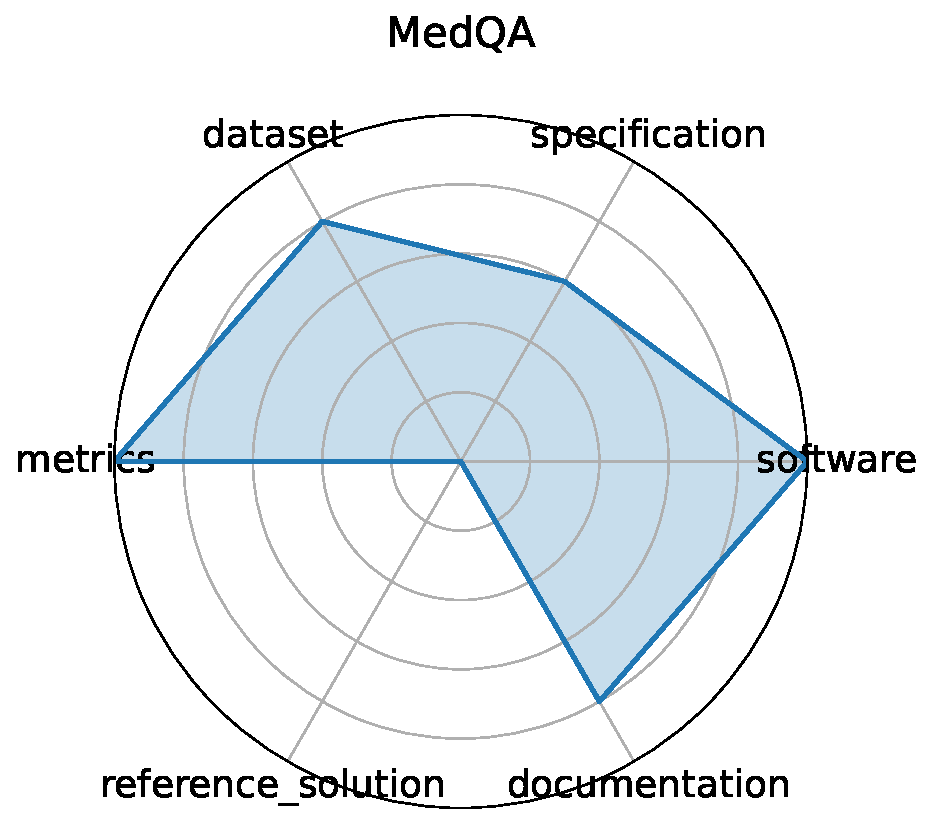
\includegraphics[width=0.15\textwidth]{medqa_radar.pdf} & MedQA & Medical Question Answering & Medical board exam QA & USMLE, diagnostic QA, medical knowledge, multilingual & Multiple choice & Medical diagnosis and knowledge retrieval & Accuracy & Neural reader, Retrieval-based QA systems & \cite{jin2020diseasedoespatienthave}\href{https://arxiv.org/abs/2009.13081}{$\Rightarrow$} \\ \hline
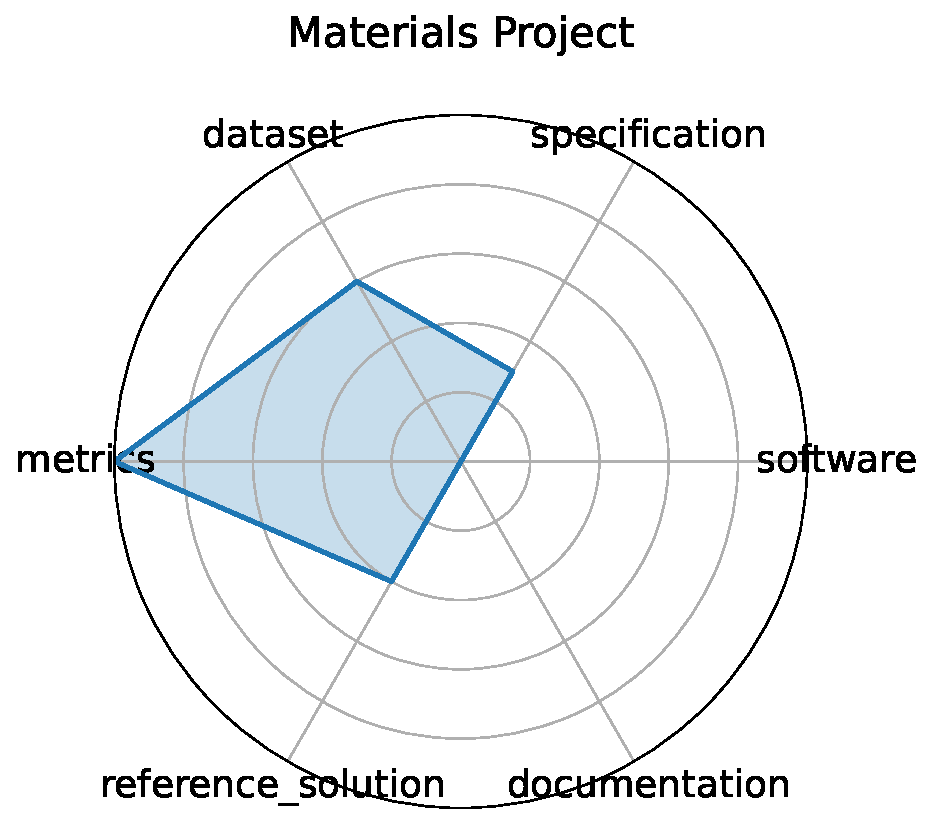
\includegraphics[width=0.15\textwidth]{materials_project_radar.pdf} & Materials Project & Materials Science & DFT-based property prediction & DFT, materials genome, high-throughput & Property prediction & Prediction of inorganic material properties & MAE, R{\textasciicircum}2 & Automatminer, Crystal Graph Neural Networks & \cite{jain2013materials}\href{https://materialsproject.org/}{$\Rightarrow$} \\ \hline
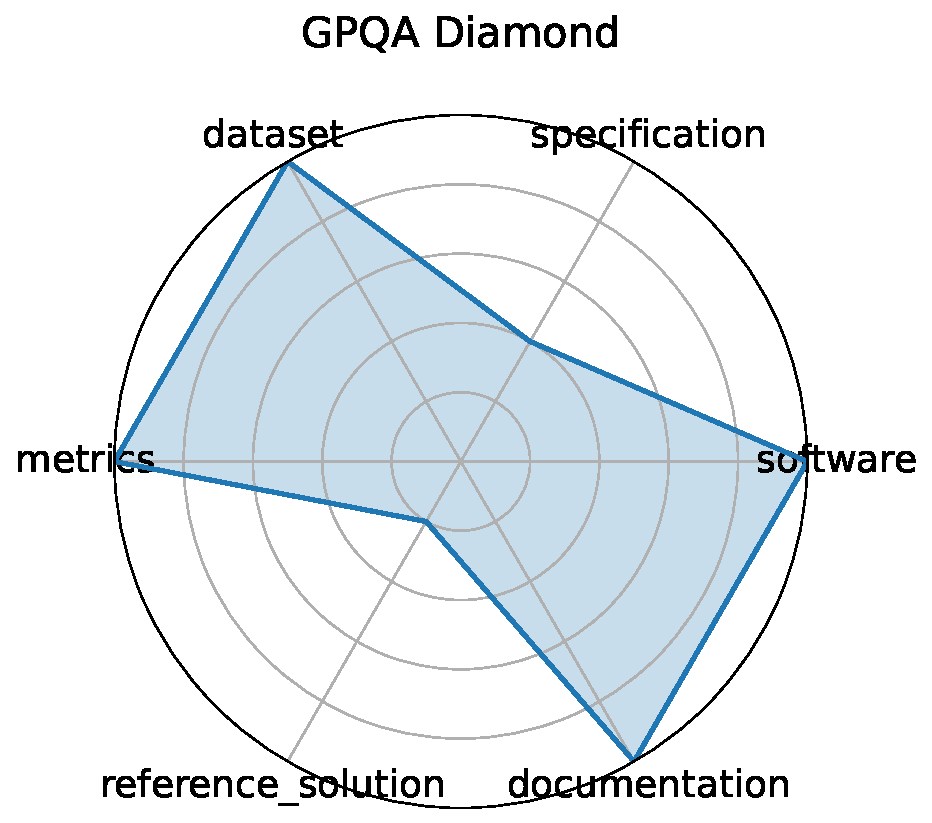
\includegraphics[width=0.15\textwidth]{gpqa_diamond_radar.pdf} & GPQA Diamond & Science & Graduate-level scientific reasoning & Google-proof, graduate-level, science QA, chemistry, physics & Multiple choice, Multi-step QA & Scientific reasoning, deep knowledge & Accuracy & o1, DeepSeek-R1 & \cite{rein2023gpqagraduatelevelgoogleproofqa}\href{https://arxiv.org/abs/2311.12022}{$\Rightarrow$} \\ \hline
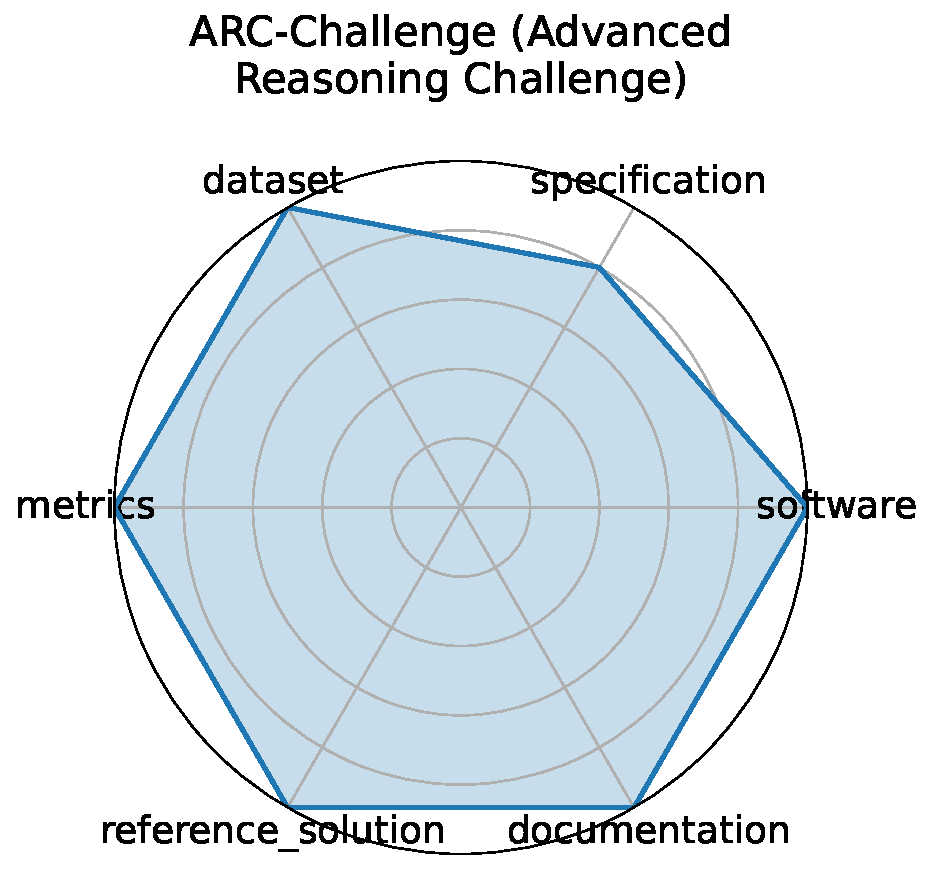
\includegraphics[width=0.15\textwidth]{arc-challenge_advanced_reasoning_challenge_radar.pdf} & ARC-Challenge (Advanced Reasoning Challenge) & Science & Grade-school science with reasoning emphasis & grade-school, science QA, challenge set, reasoning & Multiple choice & Commonsense and scientific reasoning & Accuracy & GPT-4, Claude & \cite{clark2018think}\href{https://allenai.org/data/arc}{$\Rightarrow$} \\ \hline
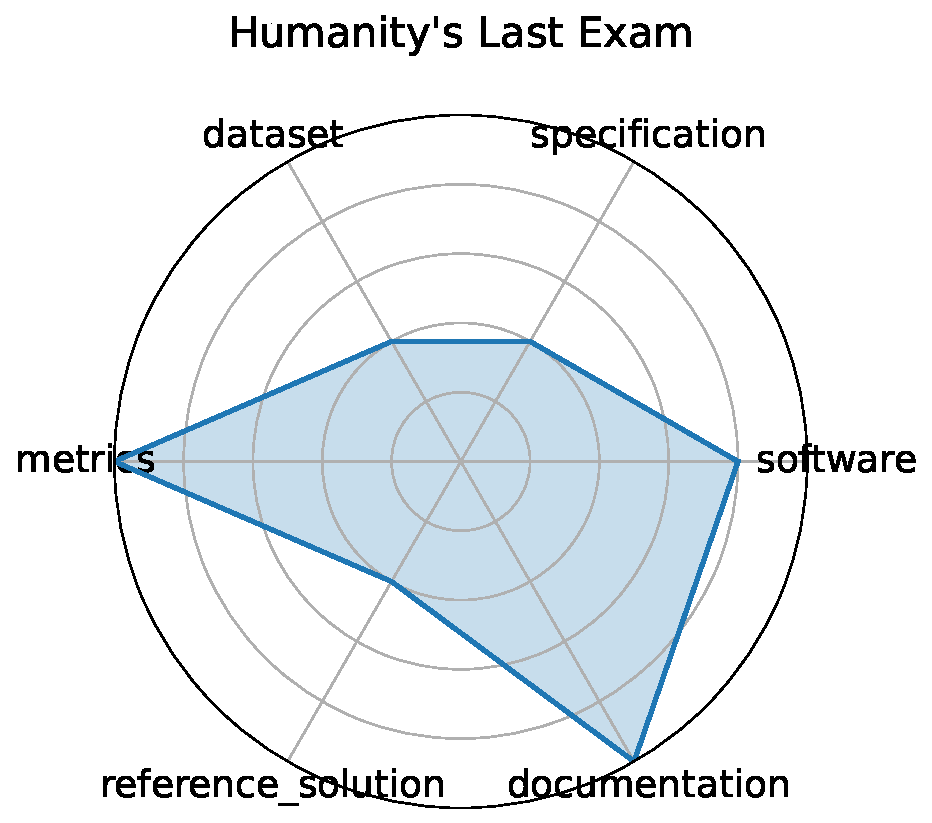
\includegraphics[width=0.15\textwidth]{humanitys_last_exam_radar.pdf} & Humanity's Last Exam & Multidomain & Broad cross-domain academic reasoning & cross-domain, academic exam, multiple-choice, multidisciplinary & Multiple choice & Cross-domain academic reasoning & Accuracy & unkown & \cite{phan2025humanitysexam}\href{https://arxiv.org/abs/2501.14249}{$\Rightarrow$} \\ \hline
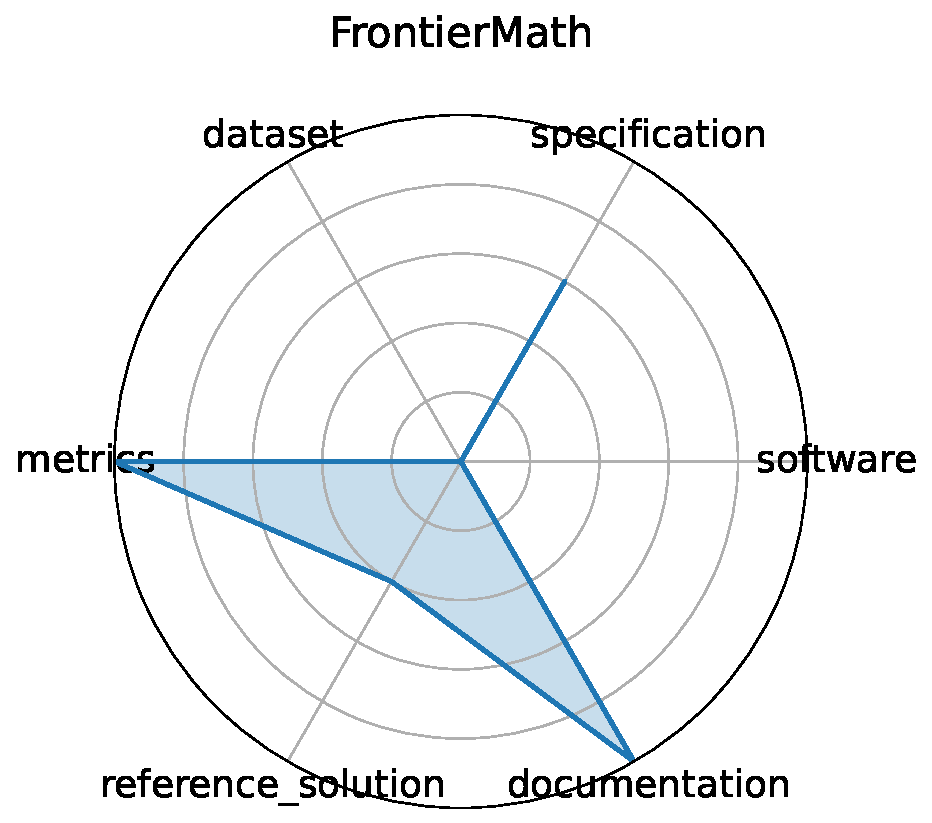
\includegraphics[width=0.15\textwidth]{frontiermath_radar.pdf} & FrontierMath & Mathematics & Challenging advanced mathematical reasoning & symbolic reasoning, number theory, algebraic geometry, category theory & Problem solving & Symbolic and abstract mathematical reasoning & Accuracy & unkown & \cite{glazer2024frontiermathbenchmarkevaluatingadvanced}\href{https://arxiv.org/abs/2411.04872}{$\Rightarrow$} \\ \hline
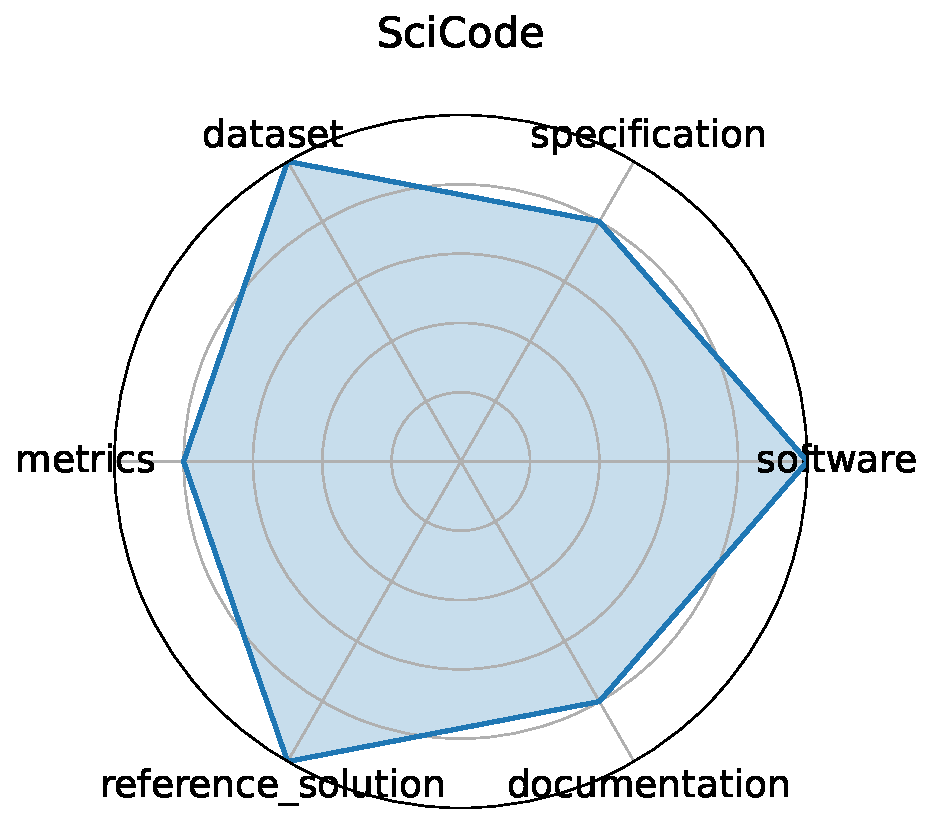
\includegraphics[width=0.15\textwidth]{scicode_radar.pdf} & SciCode & Scientific Programming & Scientific code generation and problem solving & code synthesis, scientific computing, programming benchmark & Coding & Program synthesis, scientific computing & Solve rate (\%) & Claude3.5-Sonnet & \cite{tian2024scicoderesearchcodingbenchmark}\href{https://arxiv.org/abs/2407.13168}{$\Rightarrow$} \\ \hline
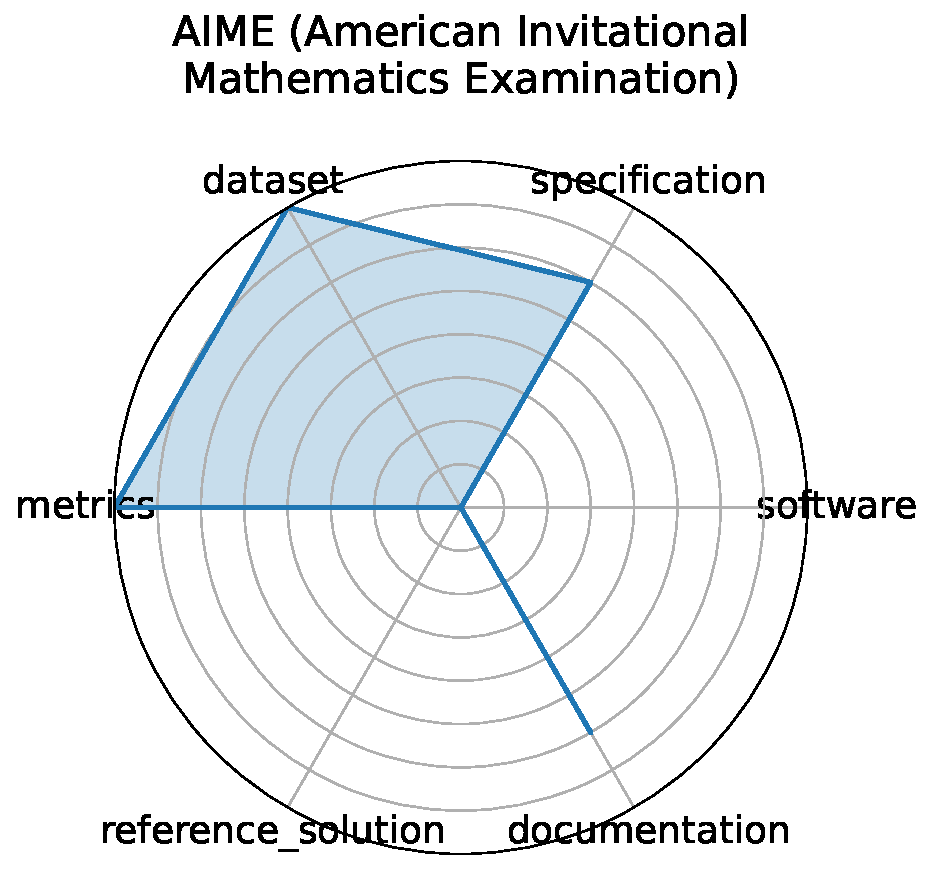
\includegraphics[width=0.15\textwidth]{aime_american_invitational_mathematics_examination_radar.pdf} & AIME (American Invitational Mathematics Examination) & Mathematics & Pre-college advanced problem solving & algebra, combinatorics, number theory, geometry & Problem solving & Mathematical problem-solving and reasoning & Accuracy & unkown & \cite{www-aime}\href{https://artofproblemsolving.com/wiki/index.php/AIME\_Problems\_and\_Solutions}{$\Rightarrow$} \\ \hline
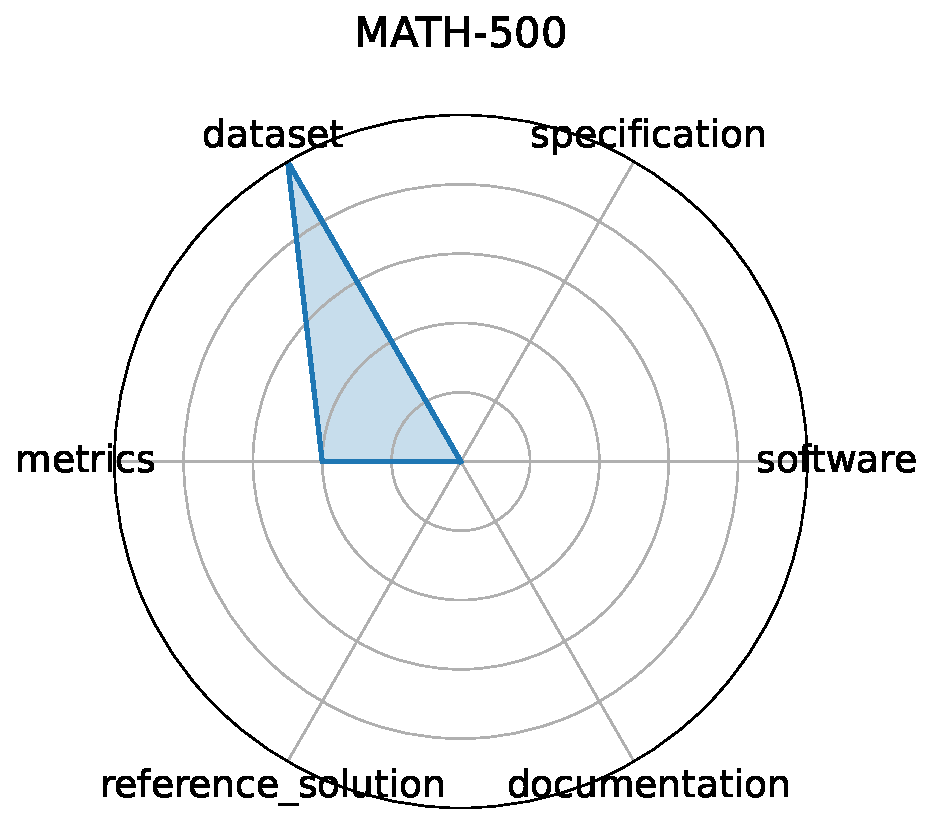
\includegraphics[width=0.15\textwidth]{math-_radar.pdf} & MATH-500 & Mathematics & Math reasoning generalization & calculus, algebra, number theory, geometry & Problem solving & Math reasoning and generalization & Accuracy & unkown & \cite{huggingface2025math500}\href{https://huggingface.co/datasets/HuggingFaceH4/MATH-500}{$\Rightarrow$} \\ \hline
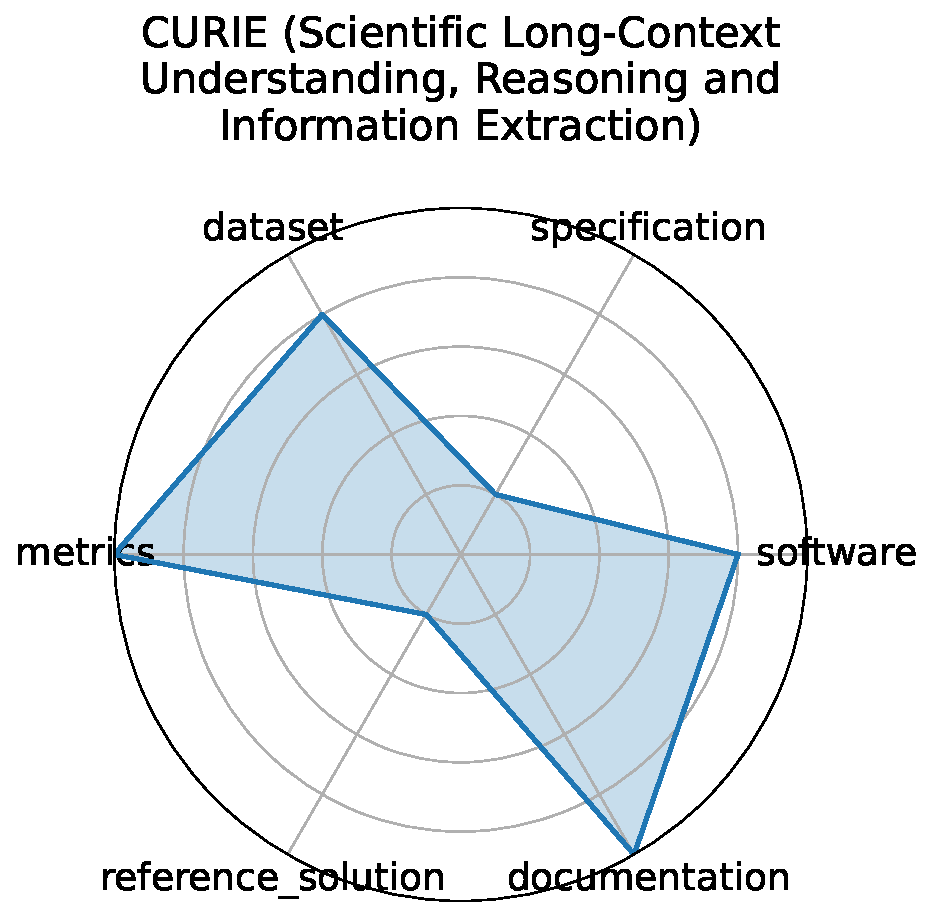
\includegraphics[width=0.15\textwidth]{curie_scientific_long-context_understanding_reasoning_and_information_extraction_radar.pdf} & CURIE (Scientific Long-Context Understanding, Reasoning and Information Extraction) & Multidomain Science & Long-context scientific reasoning & long-context, information extraction, multimodal & Information extraction, Reasoning, Concept tracking, Aggregation, Algebraic manipulation, Multimodal comprehension & Long-context understanding and scientific reasoning & Accuracy & unkown & \cite{cui2025curieevaluatingllmsmultitask}\href{https://arxiv.org/abs/2503.13517}{$\Rightarrow$} \\ \hline
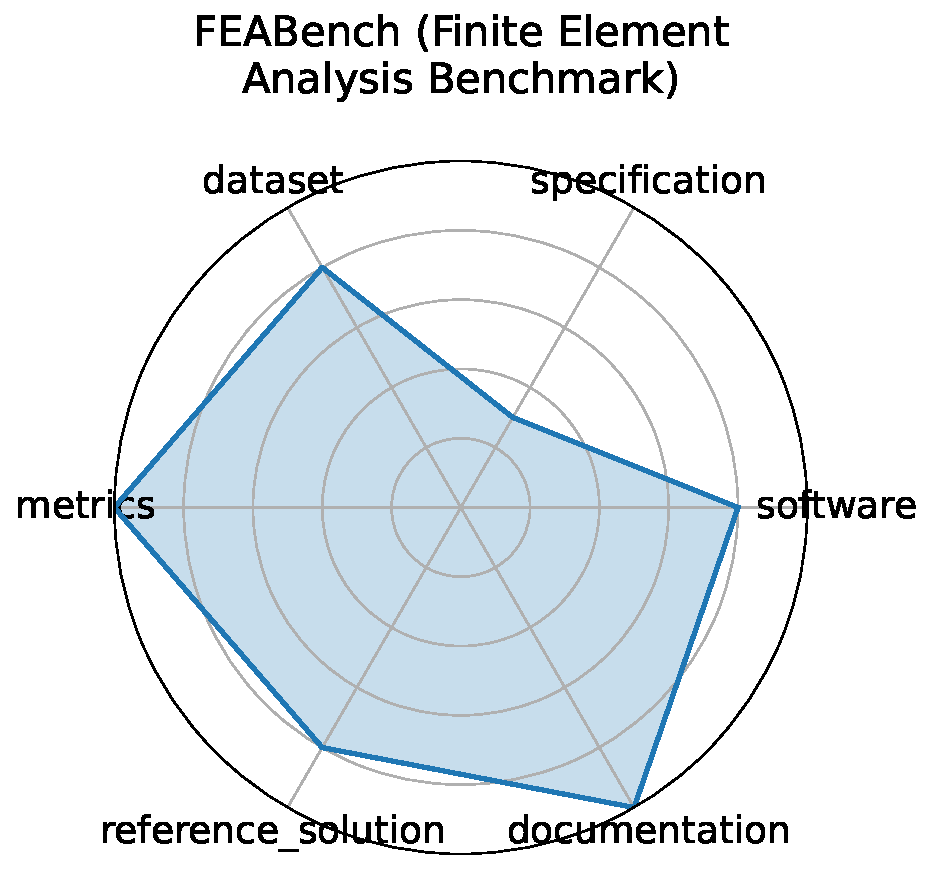
\includegraphics[width=0.15\textwidth]{feabench_finite_element_analysis_benchmark_radar.pdf} & FEABench (Finite Element Analysis Benchmark) & Computational Engineering & FEA simulation accuracy and performance & finite element, simulation, PDE & Simulation, Performance evaluation & Numerical simulation accuracy and efficiency & Solve time, Error norm & FEniCS, deal.II & \cite{mudur2025feabenchevaluatinglanguagemodels}\href{https://github.com/google/feabench}{$\Rightarrow$} \\ \hline
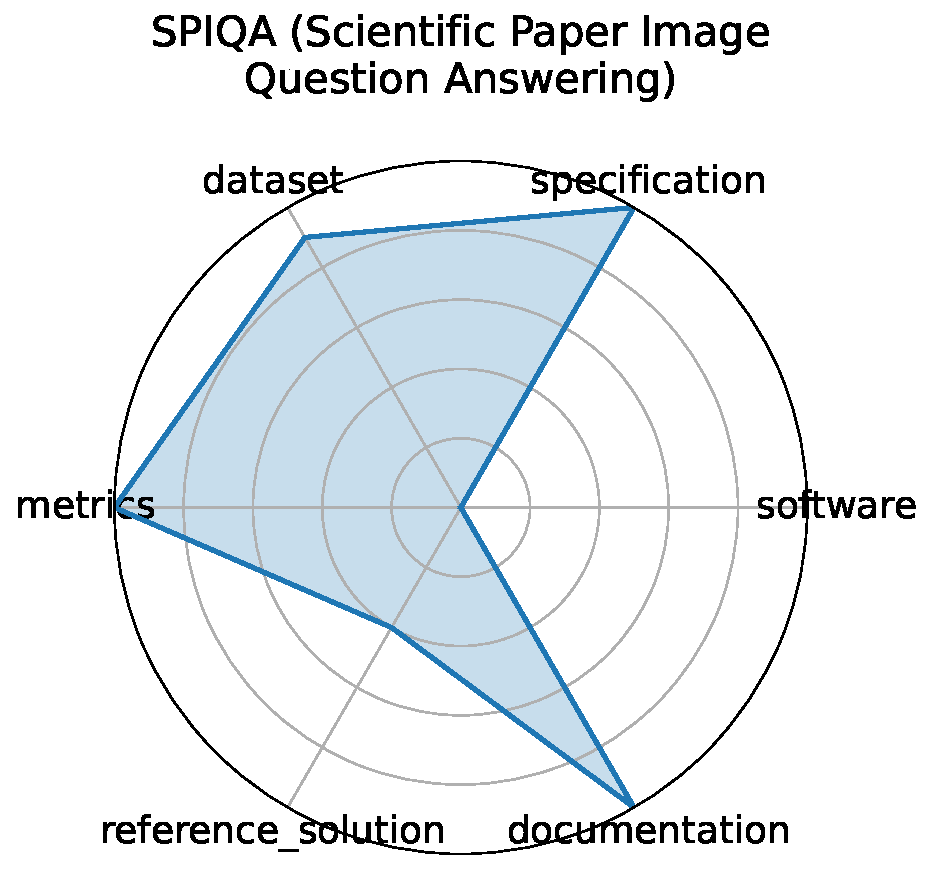
\includegraphics[width=0.15\textwidth]{spiqa_scientific_paper_image_question_answering_radar.pdf} & SPIQA (Scientific Paper Image Question Answering) & Computer Science & Multimodal QA on scientific figures & multimodal QA, figure understanding, table comprehension, chain-of-thought & Question answering, Multimodal QA, Chain-of-Thought evaluation & Visual-textual reasoning in scientific contexts & Accuracy, F1 score & Chain-of-Thought models, Multimodal QA systems & \cite{zhong2024spiqa}\href{https://arxiv.org/abs/2407.09413}{$\Rightarrow$} \\ \hline
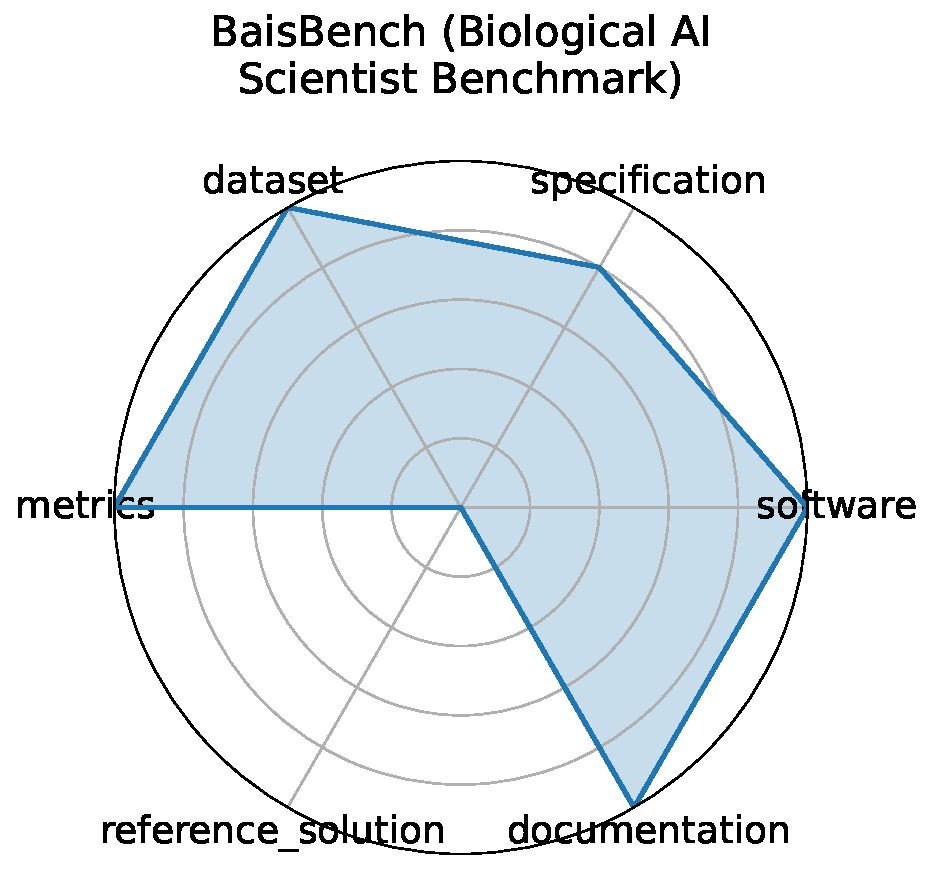
\includegraphics[width=0.15\textwidth]{baisbench_biological_ai_scientist_benchmark_radar.pdf} & BaisBench (Biological AI Scientist Benchmark) & Computational Biology & Omics-driven AI research tasks & single-cell annotation, biological QA, autonomous discovery & Cell type annotation, Multiple choice & Autonomous biological research capabilities & Annotation accuracy, QA accuracy & LLM-based AI scientist agents & \cite{luo2025benchmarkingaiscientistsomics}\href{https://arxiv.org/abs/2505.08341}{$\Rightarrow$} \\ \hline
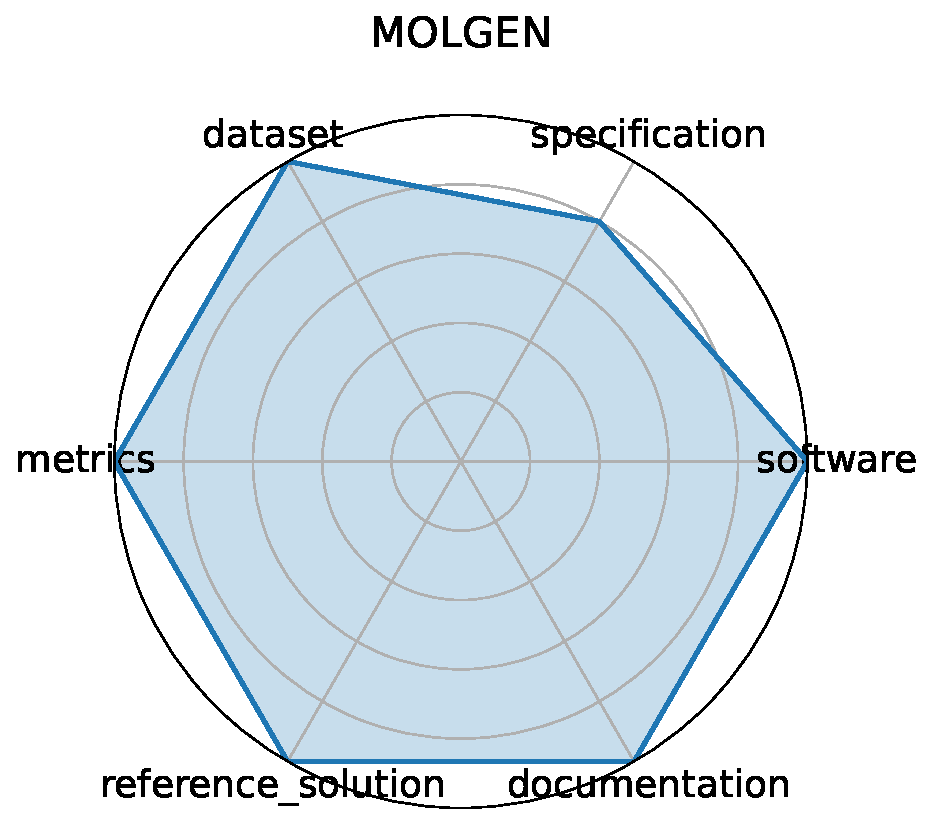
\includegraphics[width=0.15\textwidth]{molgen_radar.pdf} & MOLGEN & Computational Chemistry & Molecular generation and optimization & SELFIES, GAN, property optimization & Distribution learning, Goal-oriented generation & Generation of valid and optimized molecular structures & Validity\%, Novelty\%, QED, Docking score & MolGen & \cite{fang2024domainagnosticmoleculargenerationchemical}\href{https://github.com/zjunlp/MolGen}{$\Rightarrow$} \\ \hline
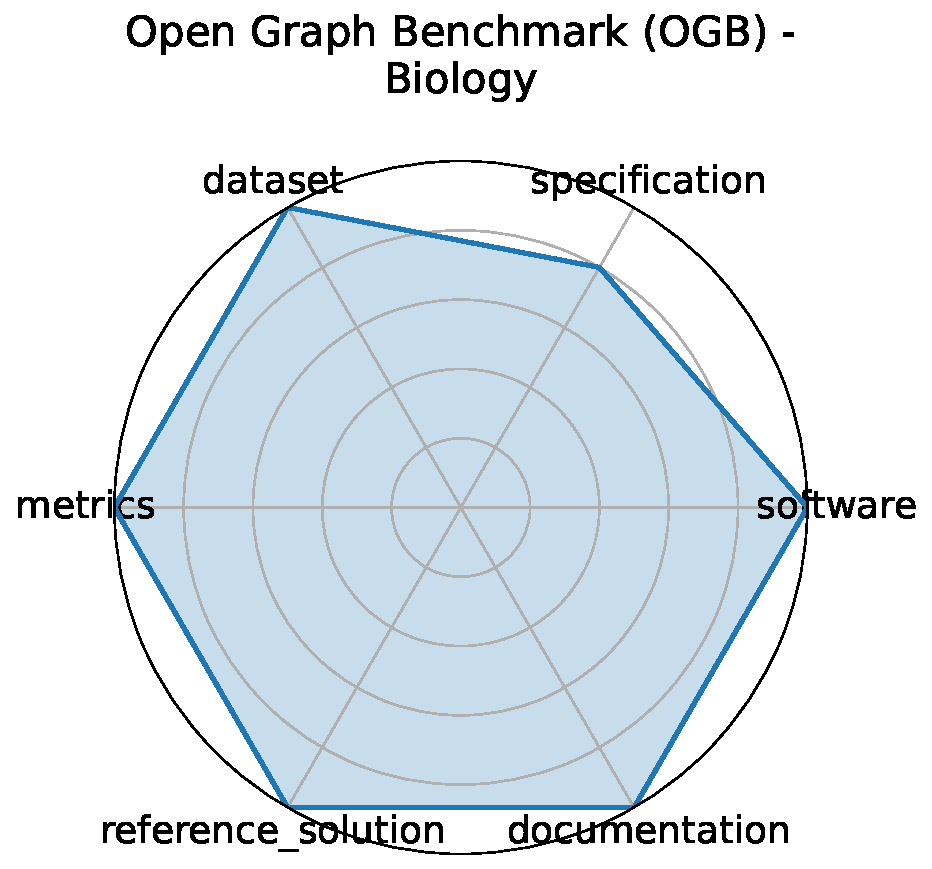
\includegraphics[width=0.15\textwidth]{open_graph_benchmark_ogb_-_biology_radar.pdf} & Open Graph Benchmark (OGB) - Biology & Graph ML & Biological graph property prediction & node prediction, link prediction, graph classification & Node property prediction, Link property prediction, Graph property prediction & Scalability and generalization in graph ML for biology & Accuracy, ROC-AUC & GCN, GraphSAGE, GAT & \cite{hu2021opengraphbenchmarkdatasets}\href{https://ogb.stanford.edu/docs/home/}{$\Rightarrow$} \\ \hline
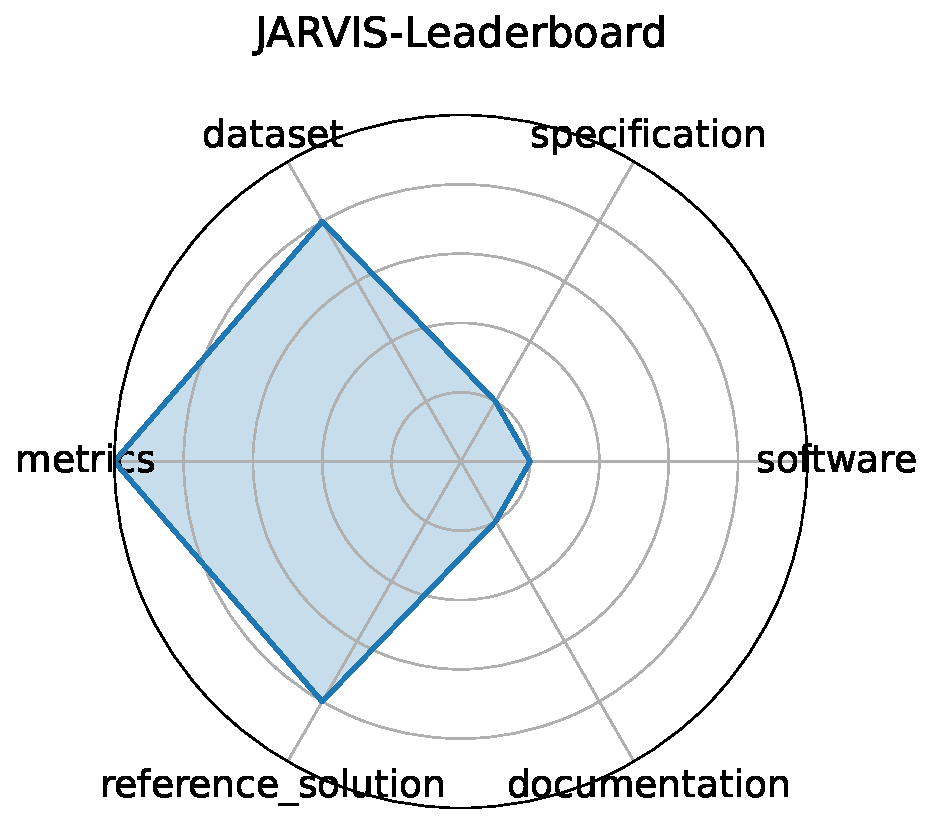
\includegraphics[width=0.15\textwidth]{jarvis-leaderboard_radar.pdf} & JARVIS-Leaderboard & Materials Science; Benchmarking & Comparative evaluation of materials design methods & leaderboards, materials methods, simulation & Method benchmarking, Leaderboard ranking & Performance comparison across diverse materials design methods & MAE, RMSE, Accuracy & unkown & \cite{choudhary2024jarvis}\href{https://arxiv.org/abs/2306.11688}{$\Rightarrow$} \\ \hline
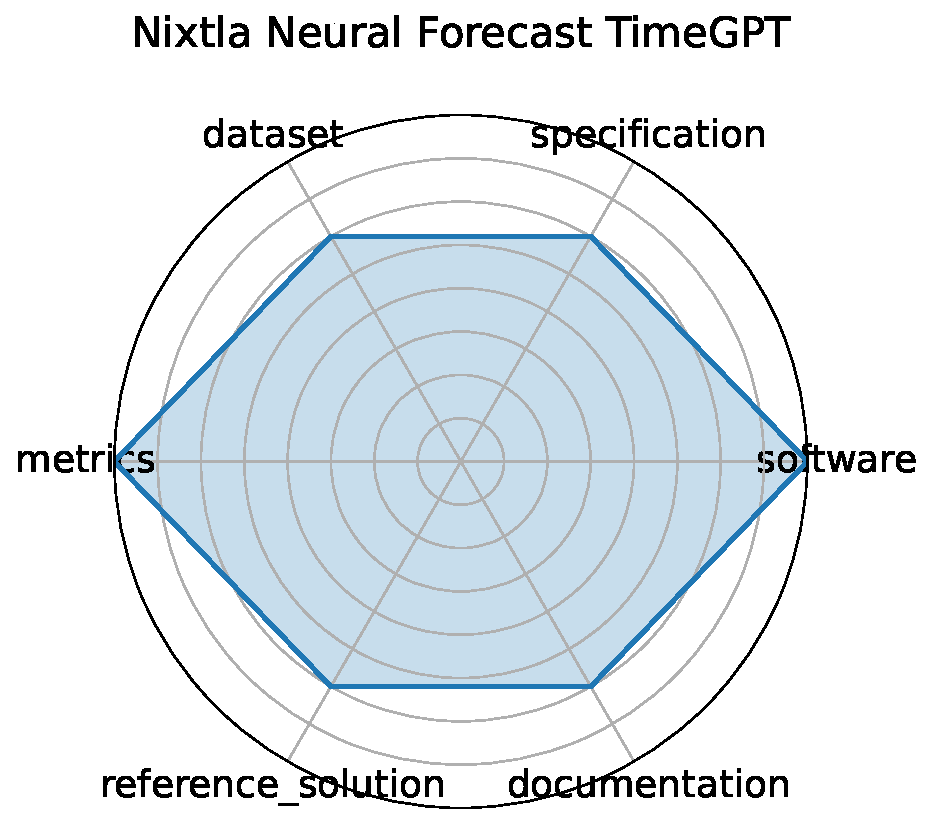
\includegraphics[width=0.15\textwidth]{nixtla_neural_forecast_timegpt_radar.pdf} & Nixtla Neural Forecast TimeGPT & Time-series; General ML & Time-series foundation model ''TimeGPT'' for forecasting and anomaly detection & TimeGPT, foundation model, time-series, generative model & Time-series forecasting, Anomaly detection & Zero-shot forecasting, anomaly detection & RMSE, Anomaly detection metrics & TimeGPT & \cite{garza2024timegpt1}\href{https://github.com/Nixtla/neuralforecast}{$\Rightarrow$} \\ \hline
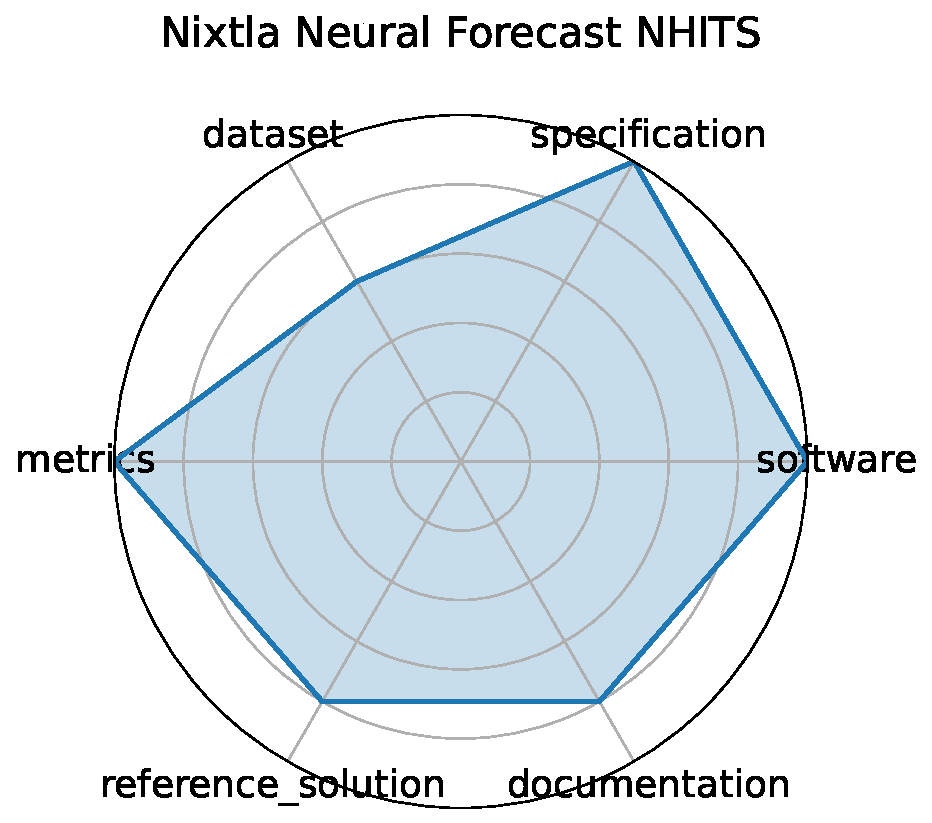
\includegraphics[width=0.15\textwidth]{nixtla_neural_forecast_nhits_radar.pdf} & Nixtla Neural Forecast NHITS & Time-series; General ML & Official NHITS implementation for long-horizon time series forecasting & NHITS, long-horizon forecasting, neural interpolation, time-series & Time-series forecasting & Accuracy, compute efficiency for long series & RMSE, MAPE & NHITS & \cite{challu2023nhits}\href{https://github.com/Nixtla/neuralforecast}{$\Rightarrow$} \\ \hline
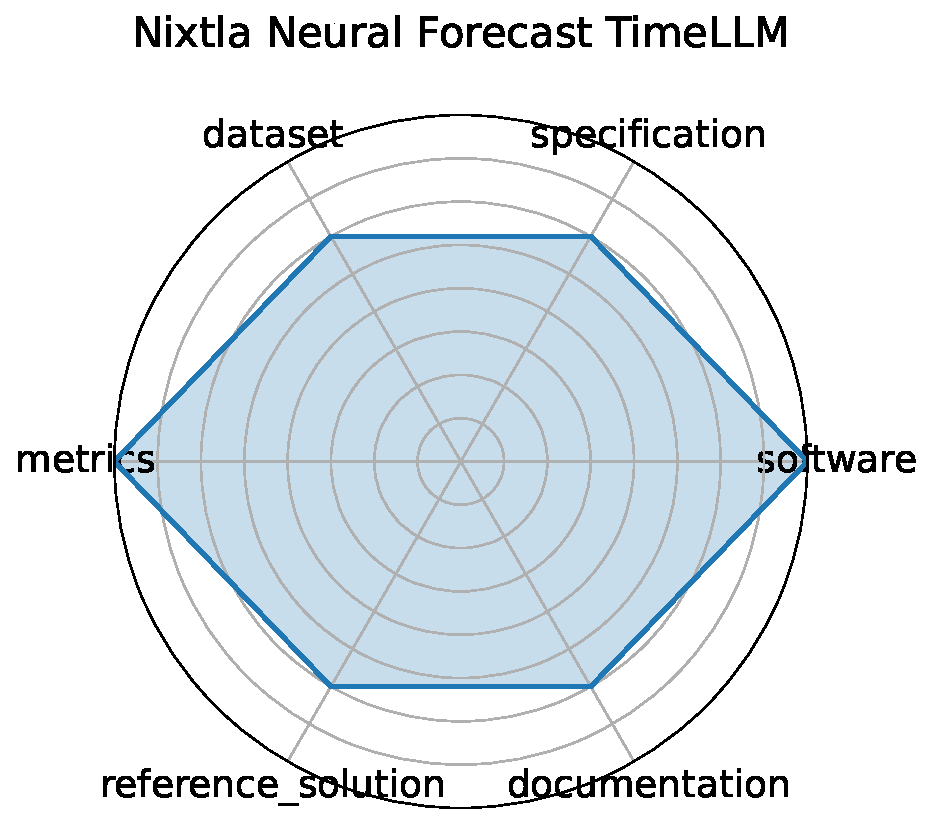
\includegraphics[width=0.15\textwidth]{nixtla_neural_forecast_timellm_radar.pdf} & Nixtla Neural Forecast TimeLLM & Time-series; General ML & Reprogramming LLMs for time series forecasting & Time-LLM, language model, time-series, reprogramming & Time-series forecasting & Model reuse via LLM, few-shot forecasting & RMSE, MAPE & Time-LLM & \cite{jin2024timellmtimeseriesforecasting}\href{https://github.com/Nixtla/neuralforecast}{$\Rightarrow$} \\ \hline
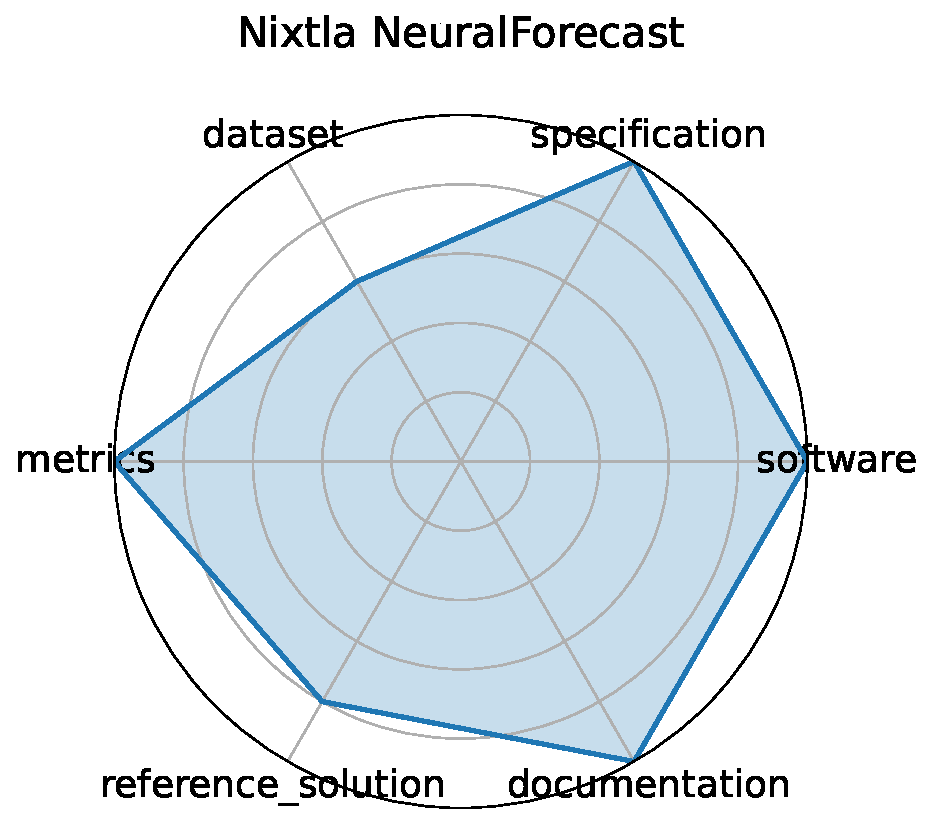
\includegraphics[width=0.15\textwidth]{nixtla_neuralforecast_radar.pdf} & Nixtla NeuralForecast & Time-series forecasting; General ML & High-performance neural forecasting library with \ensuremath{>}30 models & time-series, neural forecasting, NBEATS, NHITS, TFT, probabilistic forecasting, usability & Time-series forecasting & Forecast accuracy, interpretability, speed & RMSE, MAPE, CRPS & NBEATS, NHITS, TFT, DeepAR & \cite{olivares2022library_neuralforecast}\href{https://github.com/Nixtla/neuralforecast}{$\Rightarrow$} \\ \hline
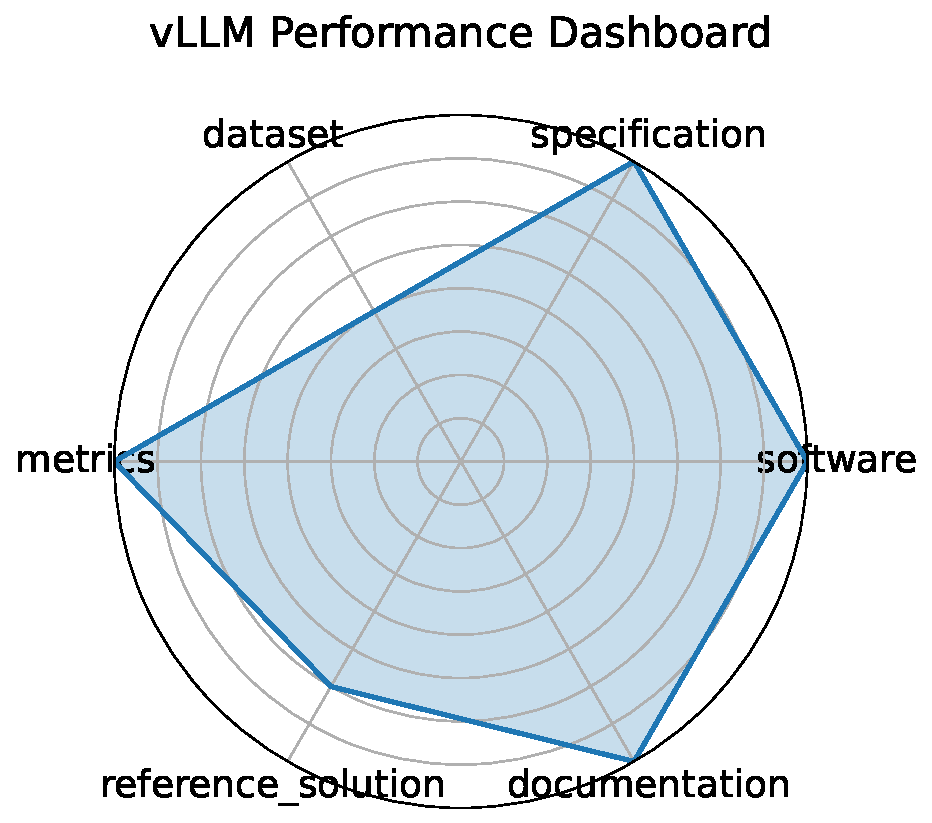
\includegraphics[width=0.15\textwidth]{vllm_performance_dashboard_radar.pdf} & vLLM Performance Dashboard & LLM; HPC/inference & Interactive dashboard showing inference performance of vLLM & Dashboard, Throughput visualization, Latency analysis, Metric tracking & Performance visualization & Throughput, latency, hardware utilization & Tokens/sec, TTFT, Memory usage & LLaMA-2, Mistral, Qwen & \cite{mo2024vllm_dashboard}\href{https://simon-mo-workspace.observablehq.cloud/vllm-dashboard-v0/}{$\Rightarrow$} \\ \hline
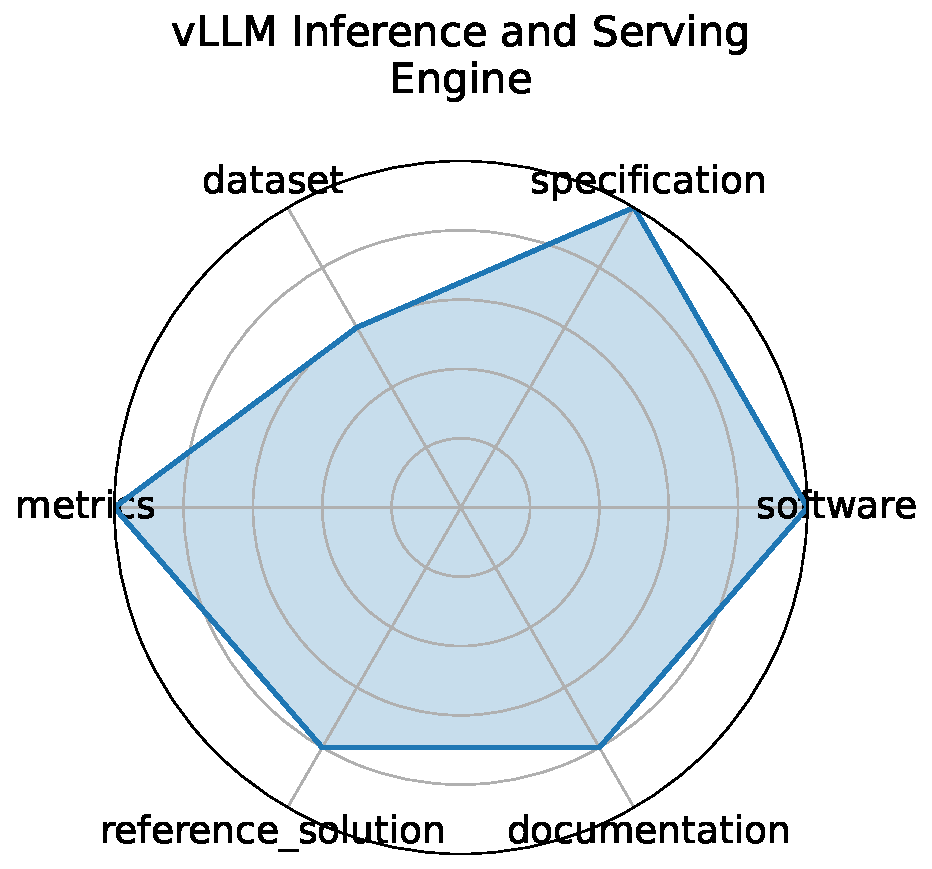
\includegraphics[width=0.15\textwidth]{vllm_inference_and_serving_engine_radar.pdf} & vLLM Inference and Serving Engine & LLM; HPC/inference & High-throughput, memory-efficient inference and serving engine for LLMs & LLM inference, PagedAttention, CUDA graph, streaming API, quantization & Inference Benchmarking & Throughput, latency, memory efficiency & Tokens/sec, Time to First Token (TTFT), Memory footprint & LLaMA, Mixtral, FlashAttention-based models & \cite{10.1145/3600006.3613165}\href{https://github.com/vllm-project/vllm/tree/main/benchmarks}{$\Rightarrow$} \\ \hline
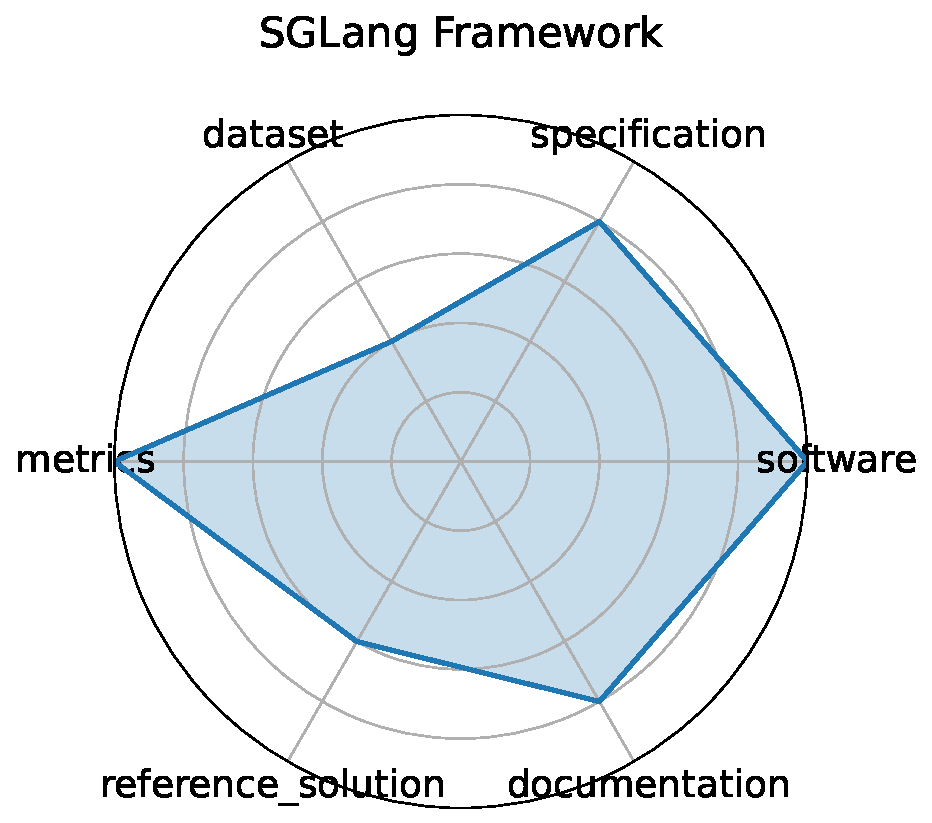
\includegraphics[width=0.15\textwidth]{sglang_framework_radar.pdf} & SGLang Framework & LLM Vision & Fast serving framework for LLMs and vision-language models & LLM serving, vision-language, RadixAttention, performance, JSON decoding & Model serving framework & Serving throughput, JSON/task-specific latency & Tokens/sec, Time-to-first-token, Throughput gain vs baseline & LLaVA, DeepSeek, Llama & \cite{zheng2024sglangefficientexecutionstructured}\href{https://github.com/sgl-project/sglang/tree/main/benchmark}{$\Rightarrow$} \\ \hline
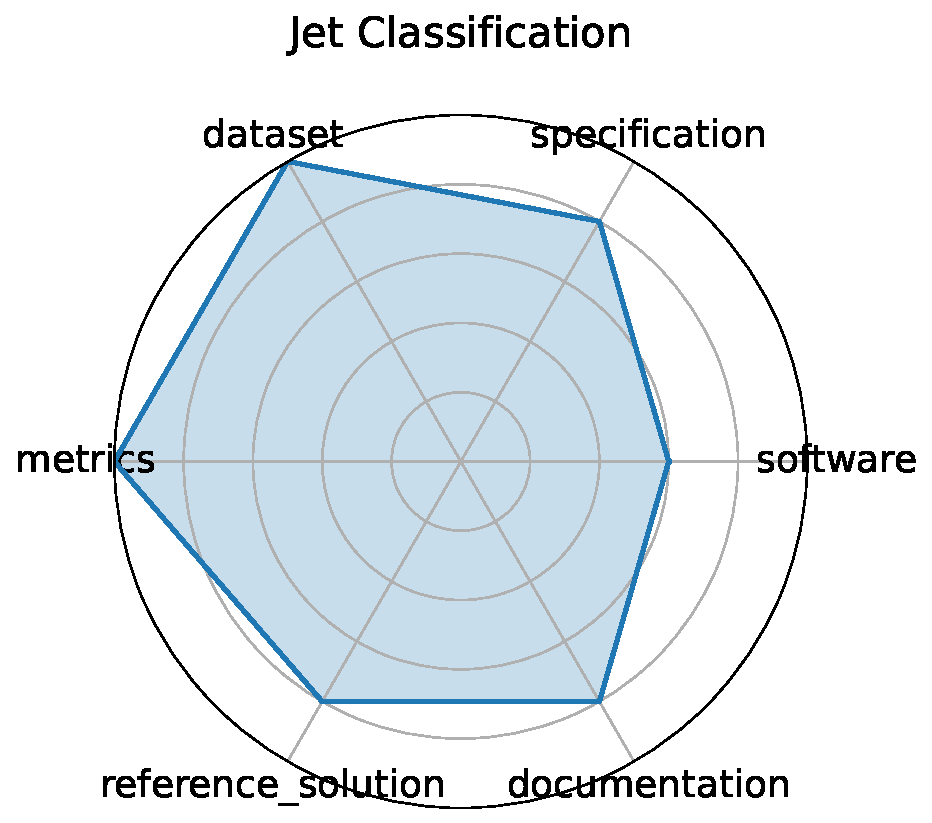
\includegraphics[width=0.15\textwidth]{jet_classification_radar.pdf} & Jet Classification & Particle Physics & Real-time classification of particle jets using HL-LHC simulation features & classification, real-time ML, jet tagging, QKeras & Classification & Real-time inference, model compression performance & Accuracy, AUC & Keras DNN, QKeras quantized DNN & \cite{duarte2022fastml}\href{https://github.com/fastmachinelearning/fastml-science/tree/main/jet-classify}{$\Rightarrow$} \\ \hline
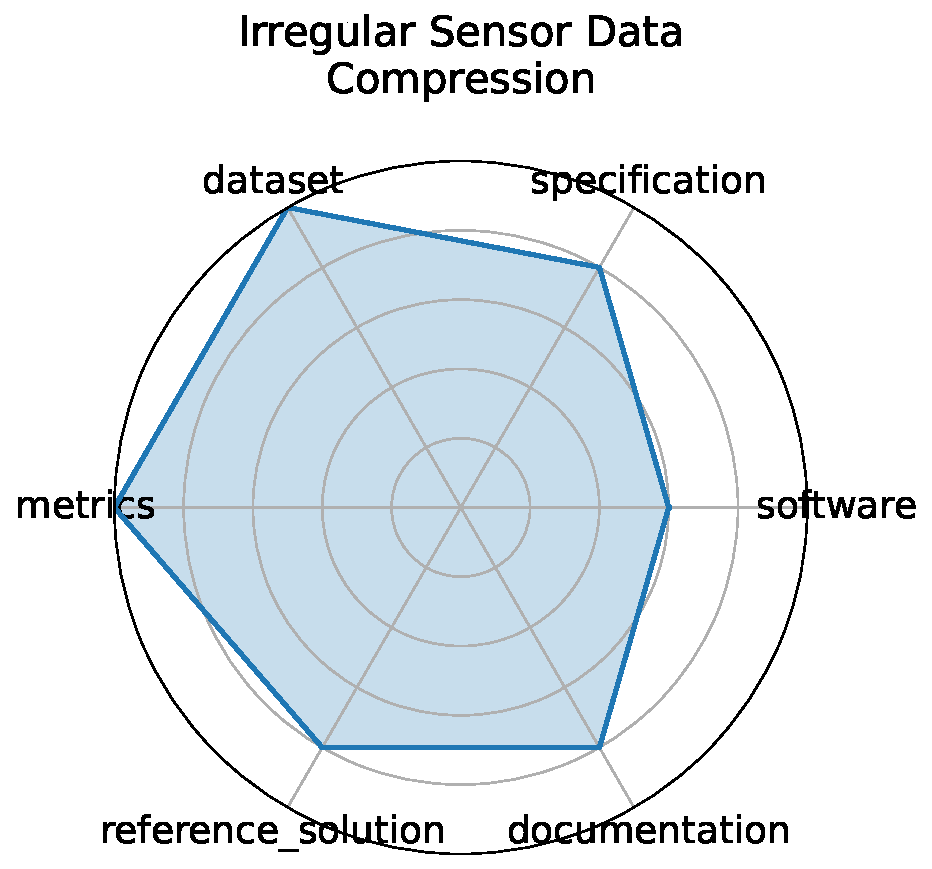
\includegraphics[width=0.15\textwidth]{irregular_sensor_data_compression_radar.pdf} & Irregular Sensor Data Compression & Particle Physics & Real-time compression of sparse sensor data with autoencoders & compression, autoencoder, sparse data, irregular sampling & Compression & Reconstruction quality, compression efficiency & MSE, Compression ratio & Autoencoder, Quantized autoencoder & \cite{duarte2022fastmlsciencebenchmarksaccelerating2}\href{https://github.com/fastmachinelearning/fastml-science/tree/main/sensor-data-compression}{$\Rightarrow$} \\ \hline
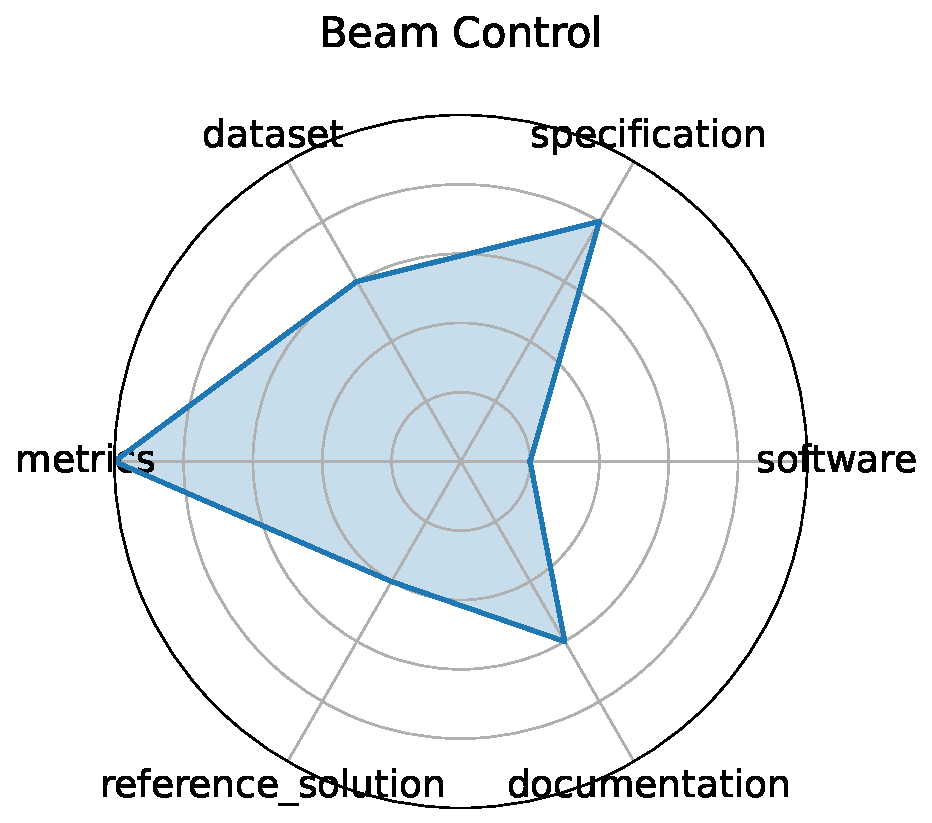
\includegraphics[width=0.15\textwidth]{beam_control_radar.pdf} & Beam Control & Accelerators and Magnets & Reinforcement learning control of accelerator beam position & RL, beam stabilization, control systems, simulation & Control & Policy performance in simulated accelerator control & Stability, Control loss & DDPG, PPO (planned) & \cite{duarte2022fastmlsciencebenchmarksaccelerating3,kafkes2021boostrdatasetacceleratorcontrol}\href{https://github.com/fastmachinelearning/fastml-science/tree/main/beam-control}{$\Rightarrow$} \\ \hline
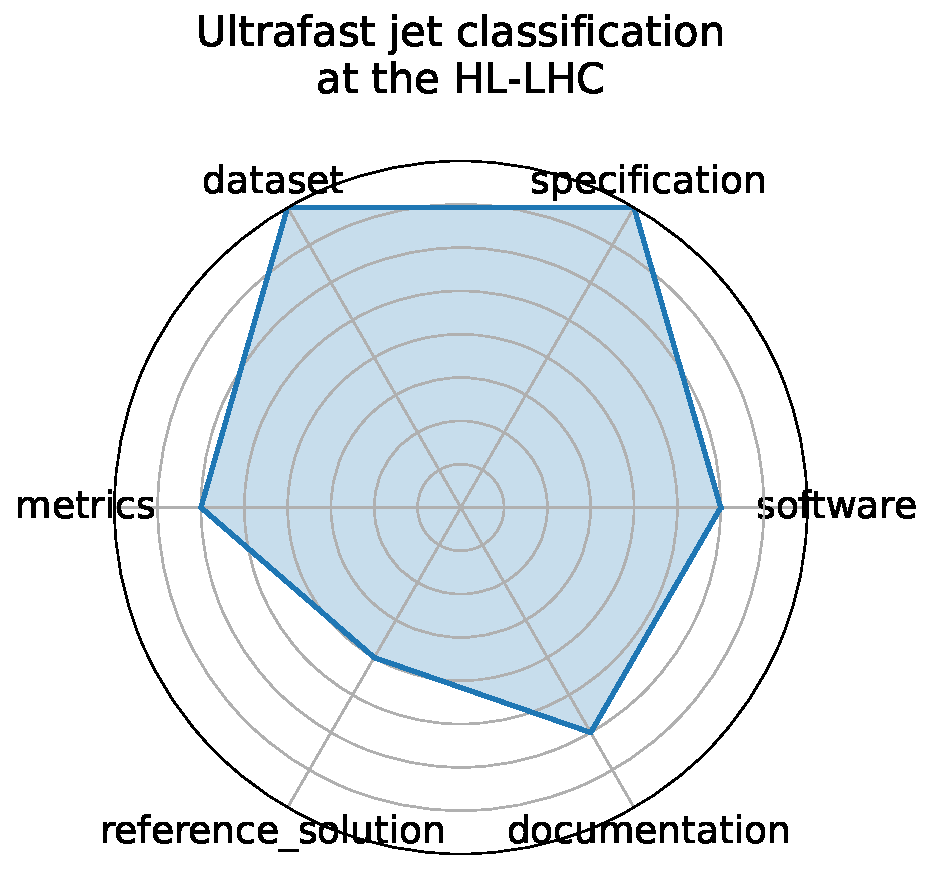
\includegraphics[width=0.15\textwidth]{ultrafast_jet_classification_at_the_hl-lhc_radar.pdf} & Ultrafast jet classification at the HL-LHC & Particle Physics & FPGA-optimized real-time jet origin classification at the HL-LHC & jet classification, FPGA, quantization-aware training, Deep Sets, Interaction Networks & Classification & Real-time inference under FPGA constraints & Accuracy, Latency, Resource utilization & MLP, Deep Sets, Interaction Network & \cite{odagiu2024ultrafastjetclassificationfpgas}\href{https://arxiv.org/pdf/2402.01876}{$\Rightarrow$} \\ \hline
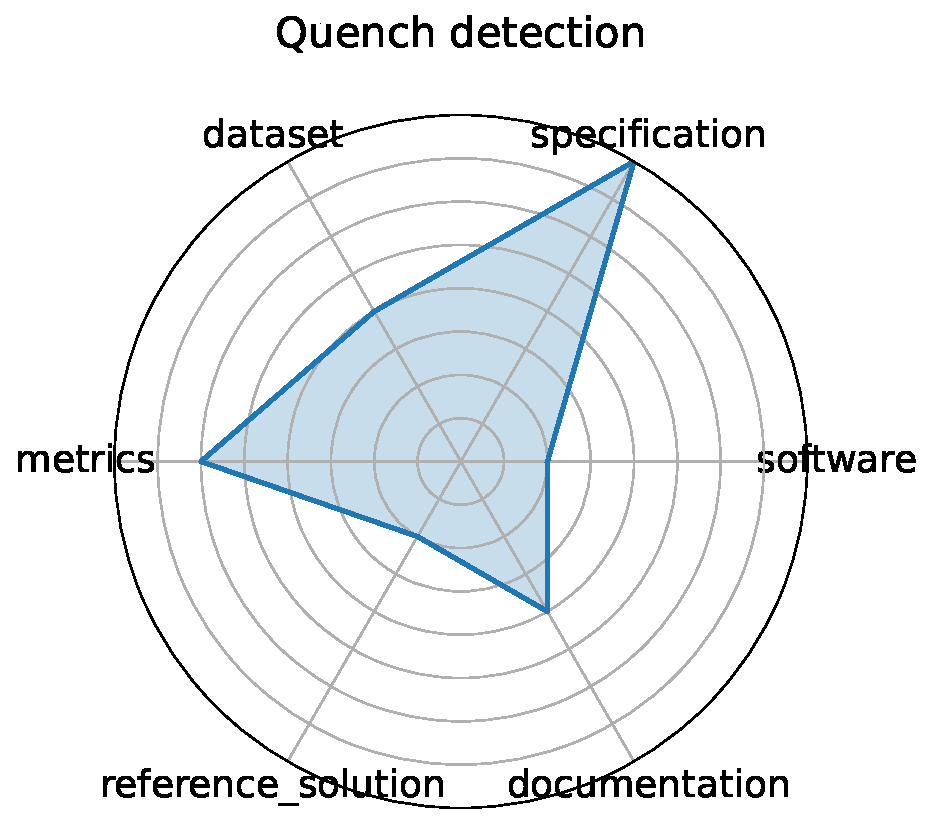
\includegraphics[width=0.15\textwidth]{quench_detection_radar.pdf} & Quench detection & Accelerators and Magnets & Real-time detection of superconducting magnet quenches using ML & quench detection, autoencoder, anomaly detection, real-time & Anomaly detection, Quench localization & Real-time anomaly detection with multi-modal sensors & ROC-AUC, Detection latency & Autoencoder, RL agents (in development) & \cite{quench2024}\href{https://indico.cern.ch/event/1387540/contributions/6153618/attachments/2948441/5182077/fast\_ml\_magnets\_2024\_final.pdf}{$\Rightarrow$} \\ \hline
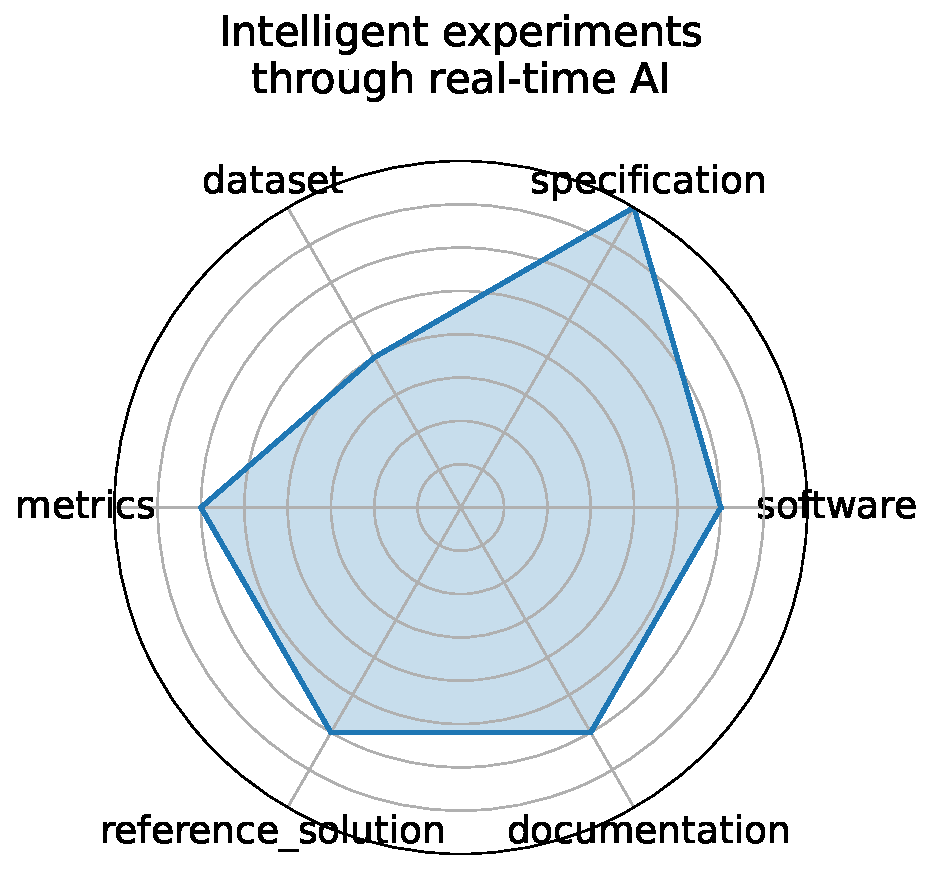
\includegraphics[width=0.15\textwidth]{intelligent_experiments_through_real-time_ai_radar.pdf} & Intelligent experiments through real-time AI & Instrumentation and Detectors; Nuclear Physics; Particle Physics & Real-time FPGA-based triggering and detector control for sPHENIX and future EIC & FPGA, Graph Neural Network, hls4ml, real-time inference, detector control & Trigger classification, Detector control, Real-time inference & Low-latency GNN inference on FPGA & Accuracy (charm and beauty detection), Latency (micros), Resource utilization (LUT/FF/BRAM/DSP) & Bipartite Graph Network with Set Transformers (BGN-ST), GarNet (edge-classifier) & \cite{kvapil2025intelligentexperimentsrealtimeai}\href{https://arxiv.org/pdf/2501.04845}{$\Rightarrow$} \\ \hline
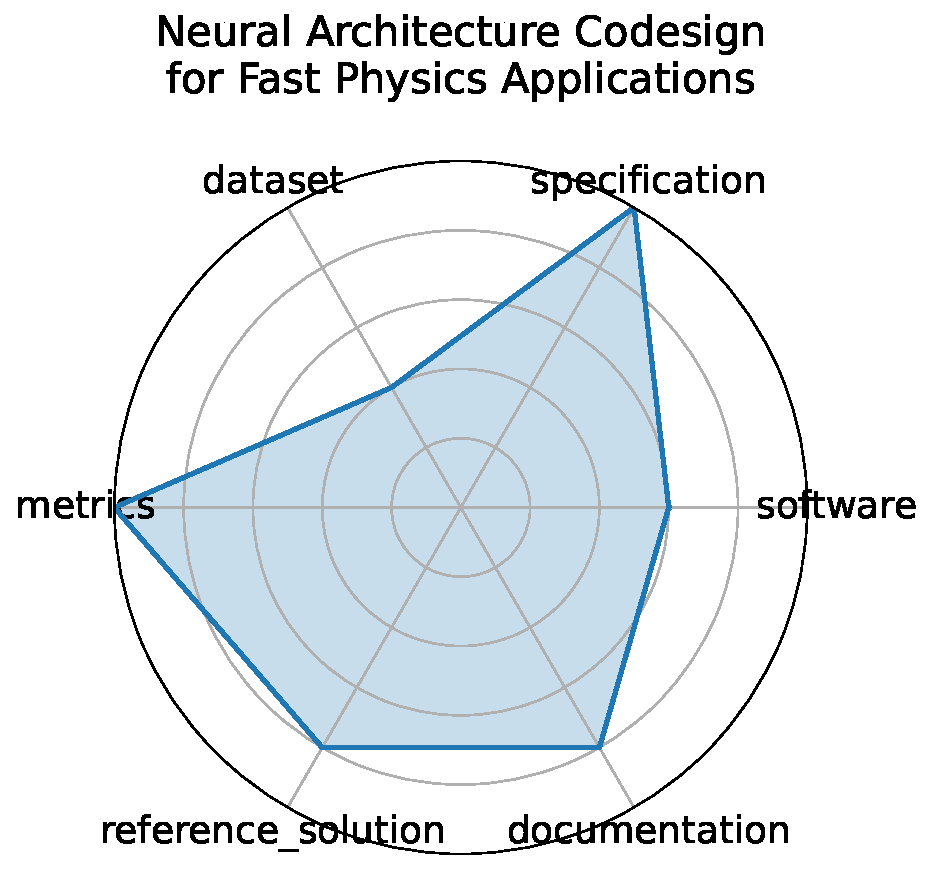
\includegraphics[width=0.15\textwidth]{neural_architecture_codesign_for_fast_physics_applications_radar.pdf} & Neural Architecture Codesign for Fast Physics Applications & Physics; Materials Science; Particle Physics & Automated neural architecture search and hardware-efficient model codesign for fast physics applications & neural architecture search, FPGA deployment, quantization, pruning, hls4ml & Classification, Peak finding & Hardware-aware model optimization; low-latency inference & Accuracy, Latency, Resource utilization & NAC-based BraggNN, NAC-optimized Deep Sets (jet) & \cite{weitz2025neuralarchitecturecodesignfast}\href{https://arxiv.org/abs/2501.05515}{$\Rightarrow$} \\ \hline
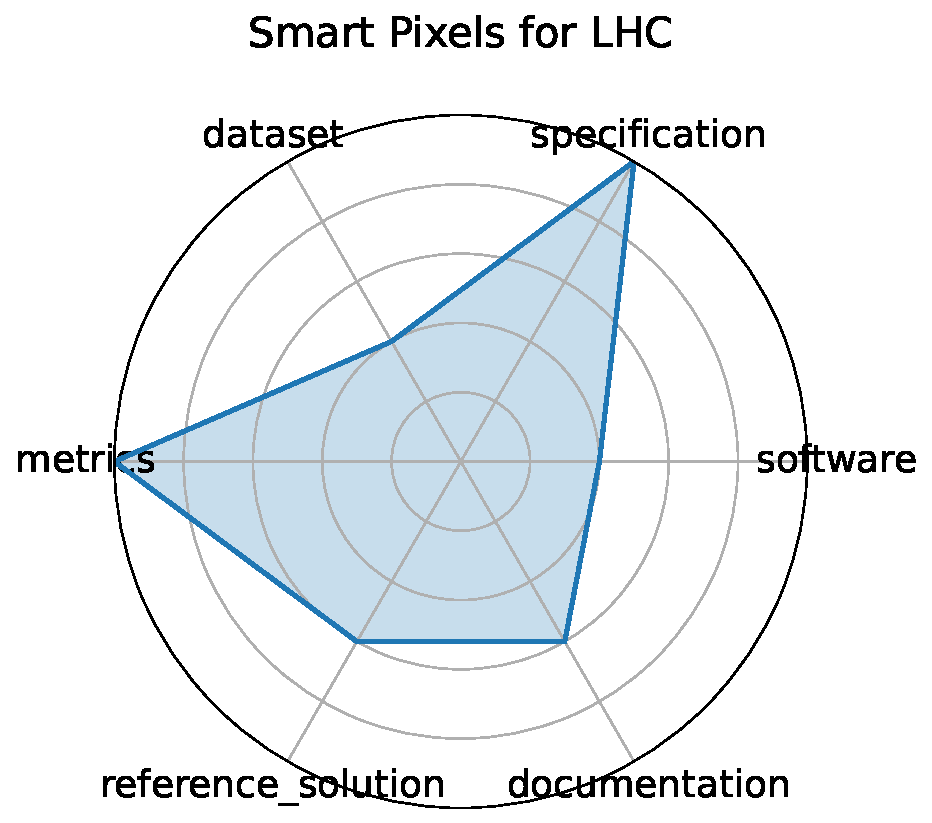
\includegraphics[width=0.15\textwidth]{smart_pixels_for_lhc_radar.pdf} & Smart Pixels for LHC & Particle Physics; Instrumentation and Detectors & On-sensor, in-pixel ML filtering for high-rate LHC pixel detectors & smart pixel, on-sensor inference, data reduction, trigger & Image Classification, Data filtering & On-chip, low-power inference; data reduction & Data rejection rate, Power per pixel & 2-layer pixel NN & \cite{parpillon2024smartpixelsinpixelai}\href{https://arxiv.org/abs/2406.14860}{$\Rightarrow$} \\ \hline
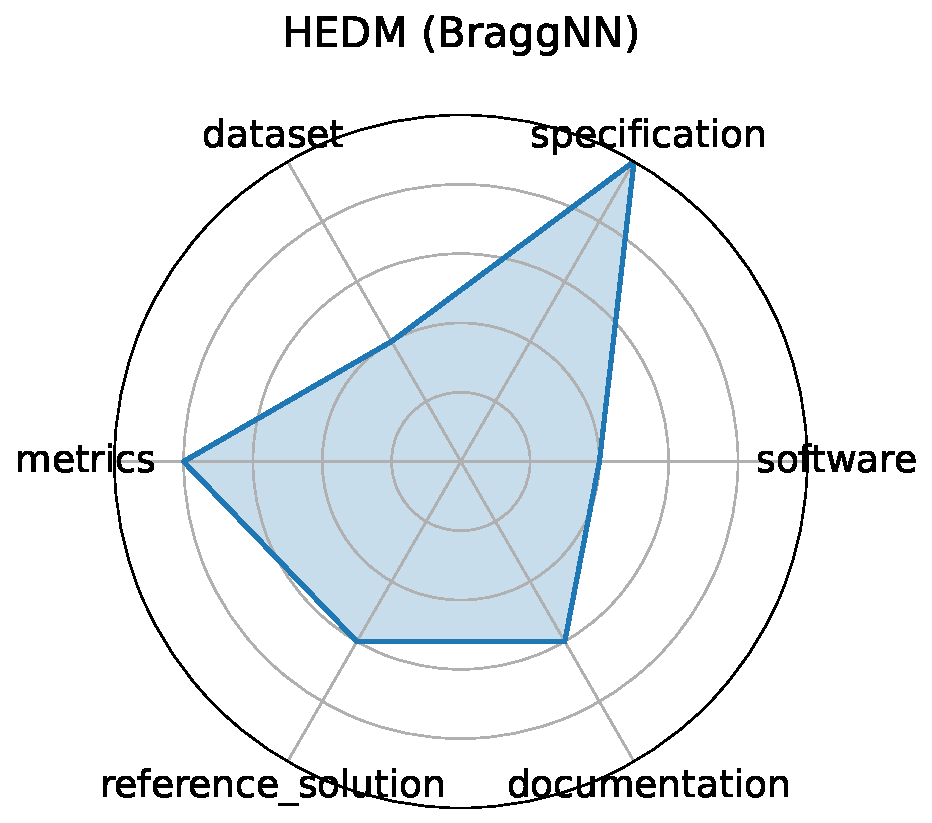
\includegraphics[width=0.15\textwidth]{hedm_braggnn_radar.pdf} & HEDM (BraggNN) & Material Science & Fast Bragg peak analysis using deep learning in diffraction microscopy & BraggNN, diffraction, peak finding, HEDM & Peak detection & High-throughput peak localization & Localization accuracy, Inference time & BraggNN & \cite{liu2021braggnnfastxraybragg}\href{https://arxiv.org/abs/2008.08198}{$\Rightarrow$} \\ \hline
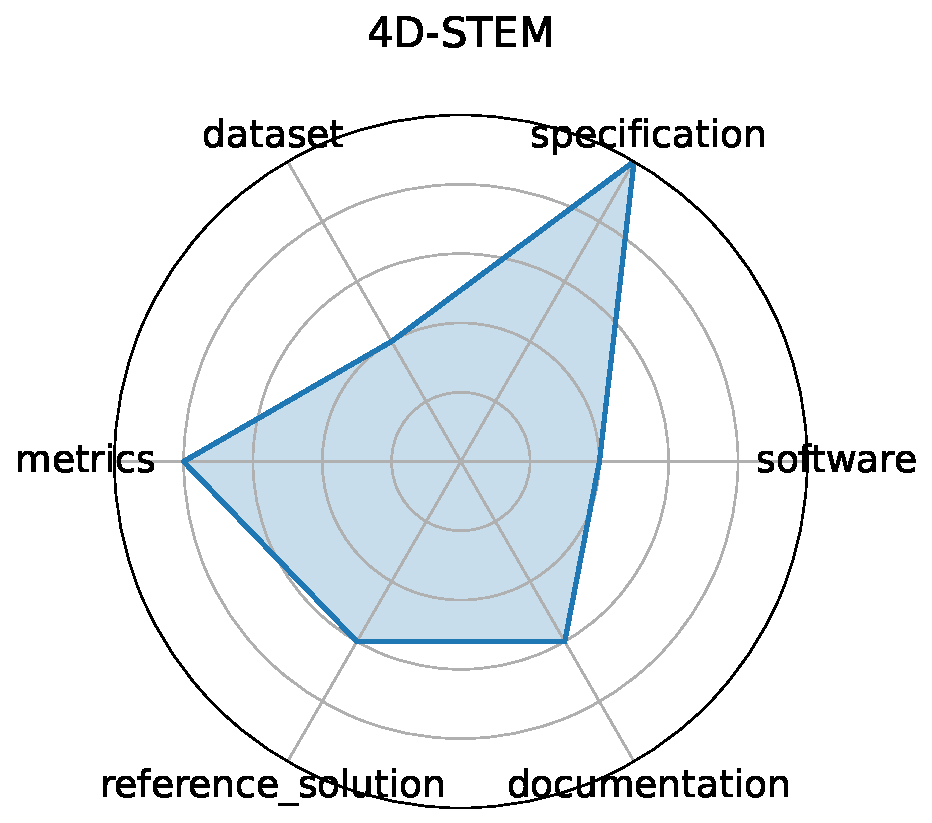
\includegraphics[width=0.15\textwidth]{d-stem_radar.pdf} & 4D-STEM & Material Science & Real-time ML for scanning transmission electron microscopy & 4D-STEM, electron microscopy, real-time, image processing & Image Classification, Streamed data inference & Real-time large-scale microscopy inference & Classification accuracy, Throughput & CNN models (prototype) & \cite{qin2023extremely}\href{https://openreview.net/pdf?id=7yt3N0o0W9}{$\Rightarrow$} \\ \hline
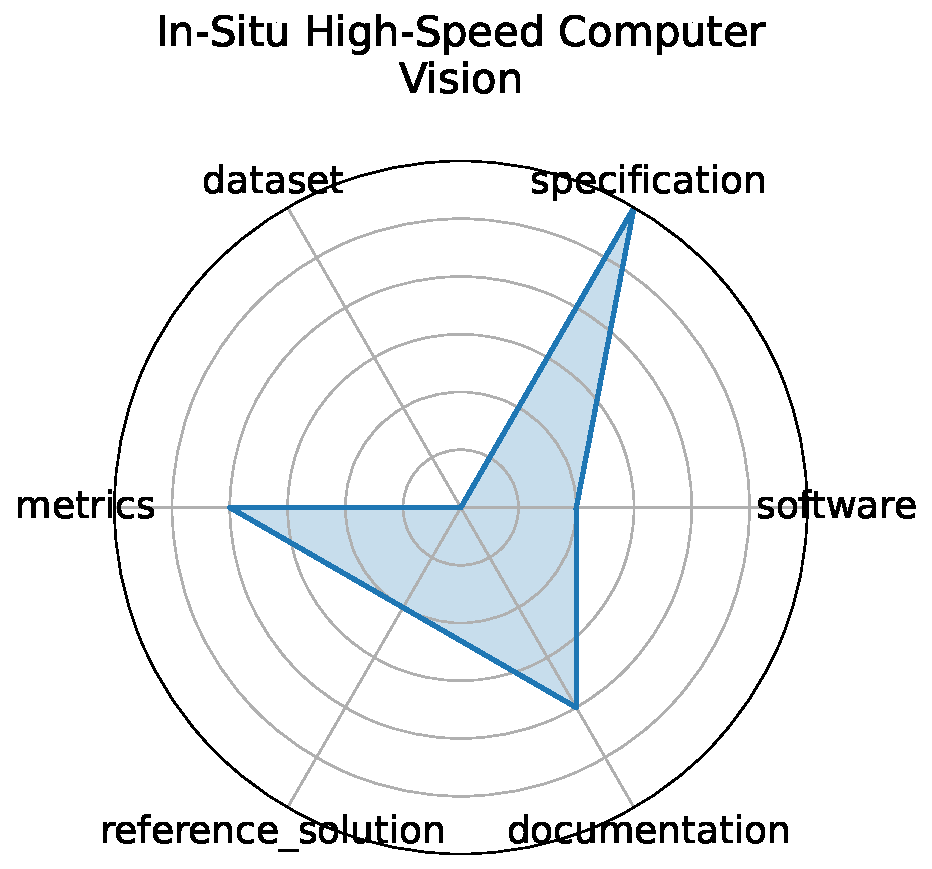
\includegraphics[width=0.15\textwidth]{in-situ_high-speed_computer_vision_radar.pdf} & In-Situ High-Speed Computer Vision & Fusion/Plasma & Real-time image classification for in-situ plasma diagnostics & plasma, in-situ vision, real-time ML & Image Classification & Real-time diagnostic inference & Accuracy, FPS & CNN & \cite{wei2024lowlatencyopticalbasedmode}\href{https://arxiv.org/abs/2312.00128}{$\Rightarrow$} \\ \hline
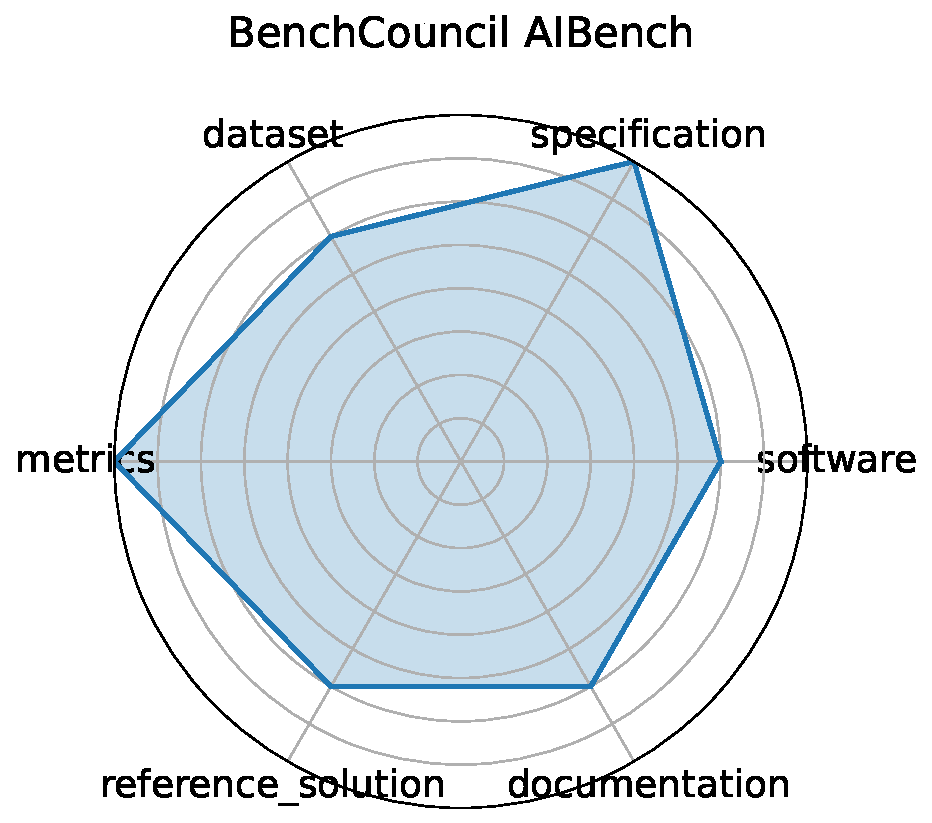
\includegraphics[width=0.15\textwidth]{benchcouncil_aibench_radar.pdf} & BenchCouncil AIBench & General & End-to-end AI benchmarking across micro, component, and application levels & benchmarking, AI systems, application-level evaluation & Training, Inference, End-to-end AI workloads & System-level AI workload performance & Throughput, Latency, Accuracy & ResNet, BERT, GANs, Recommendation systems & \cite{gao2019aibenchindustrystandardinternet}\href{https://www.benchcouncil.org/AIBench/}{$\Rightarrow$} \\ \hline
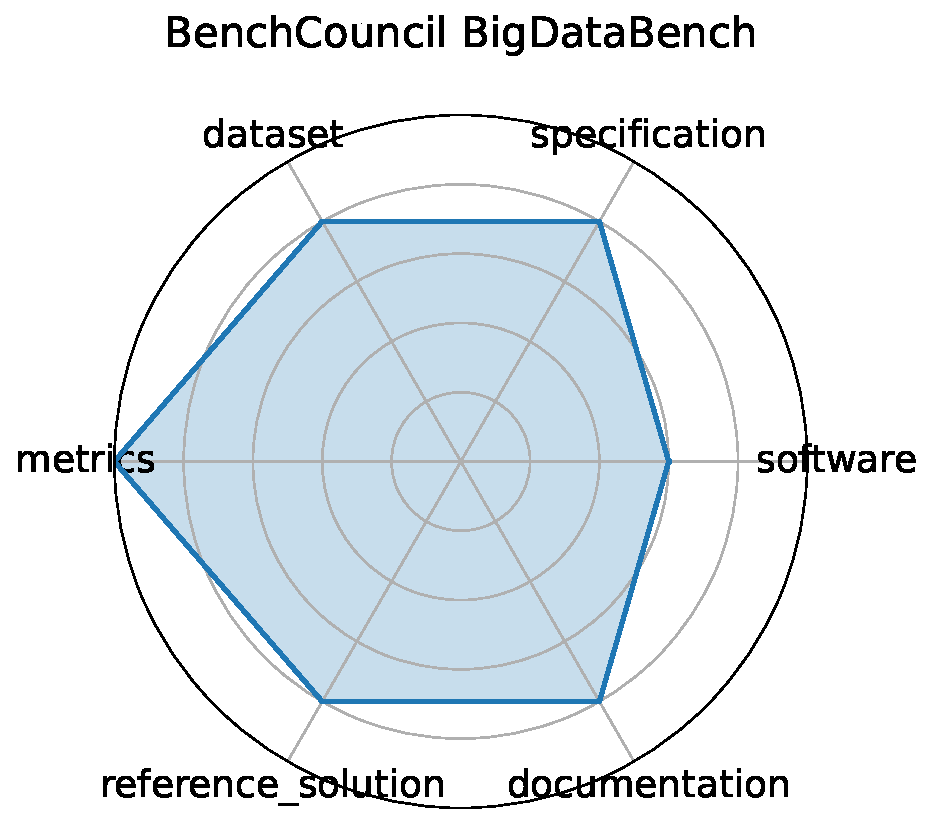
\includegraphics[width=0.15\textwidth]{benchcouncil_bigdatabench_radar.pdf} & BenchCouncil BigDataBench & General & Big data and AI benchmarking across structured, semi-structured, and unstructured data workloads & big data, AI benchmarking, data analytics & Data preprocessing, Inference, End-to-end data pipelines & Data processing and AI model inference performance at scale & Data throughput, Latency, Accuracy & CNN, LSTM, SVM, XGBoost & \cite{gao2018bigdatabenchscalableunifiedbig}\href{https://www.benchcouncil.org/BigDataBench/}{$\Rightarrow$} \\ \hline
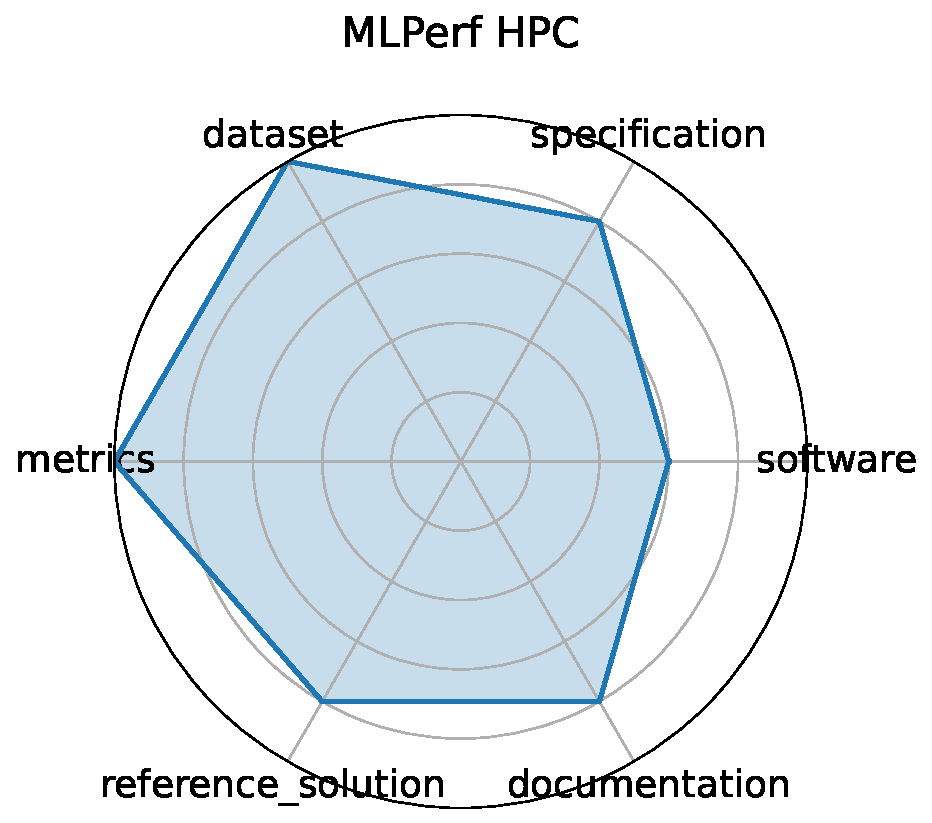
\includegraphics[width=0.15\textwidth]{mlperf_hpc_radar.pdf} & MLPerf HPC & Cosmology, Climate, Protein Structure, Catalysis & Scientific ML training and inference on HPC systems & HPC, training, inference, scientific ML & Training, Inference & Scaling efficiency, training time, model accuracy on HPC & Training time, Accuracy, GPU utilization & CosmoFlow, DeepCAM, OpenCatalyst & \cite{farrell2021mlperfhpcholisticbenchmark}\href{https://github.com/mlcommons/hpc}{$\Rightarrow$} \\ \hline
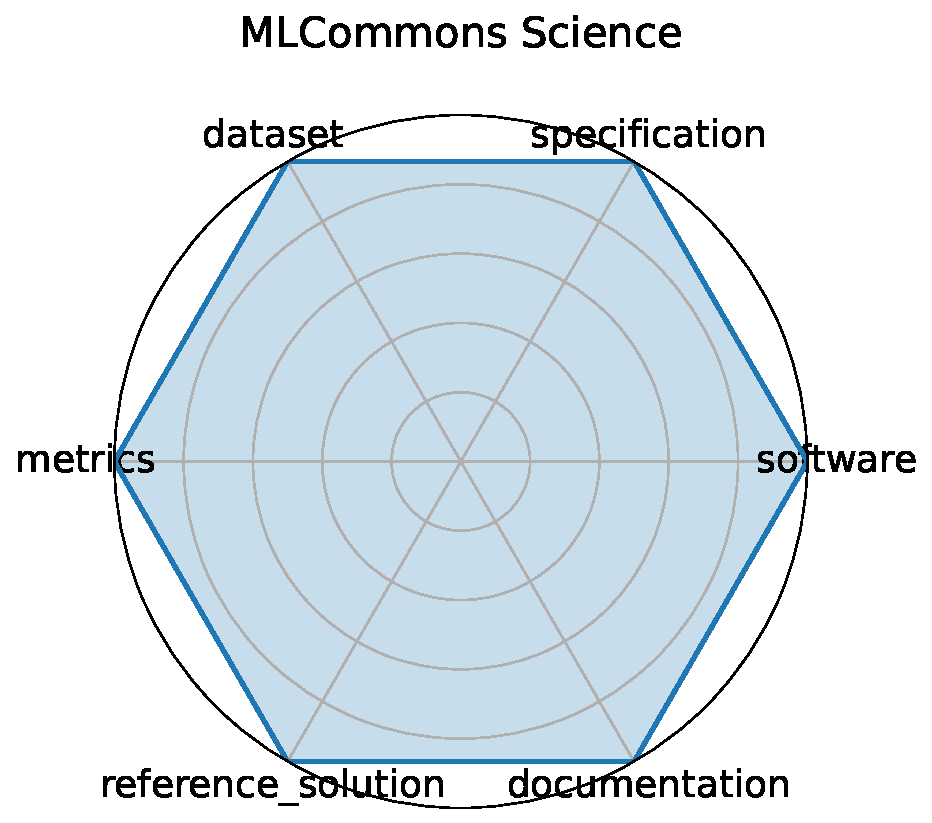
\includegraphics[width=0.15\textwidth]{mlcommons_science_radar.pdf} & MLCommons Science & Earthquake, Satellite Image, Drug Discovery, Electron Microscope, CFD & AI benchmarks for scientific applications including time-series, imaging, and simulation & science AI, benchmark, MLCommons, HPC & Time-series analysis, Image classification, Simulation surrogate modeling & Inference accuracy, simulation speed-up, generalization & MAE, Accuracy, Speedup vs simulation & CNN, GNN, Transformer & \cite{10.1007/978-3-031-23220-6_4}\href{https://github.com/mlcommons/science}{$\Rightarrow$} \\ \hline
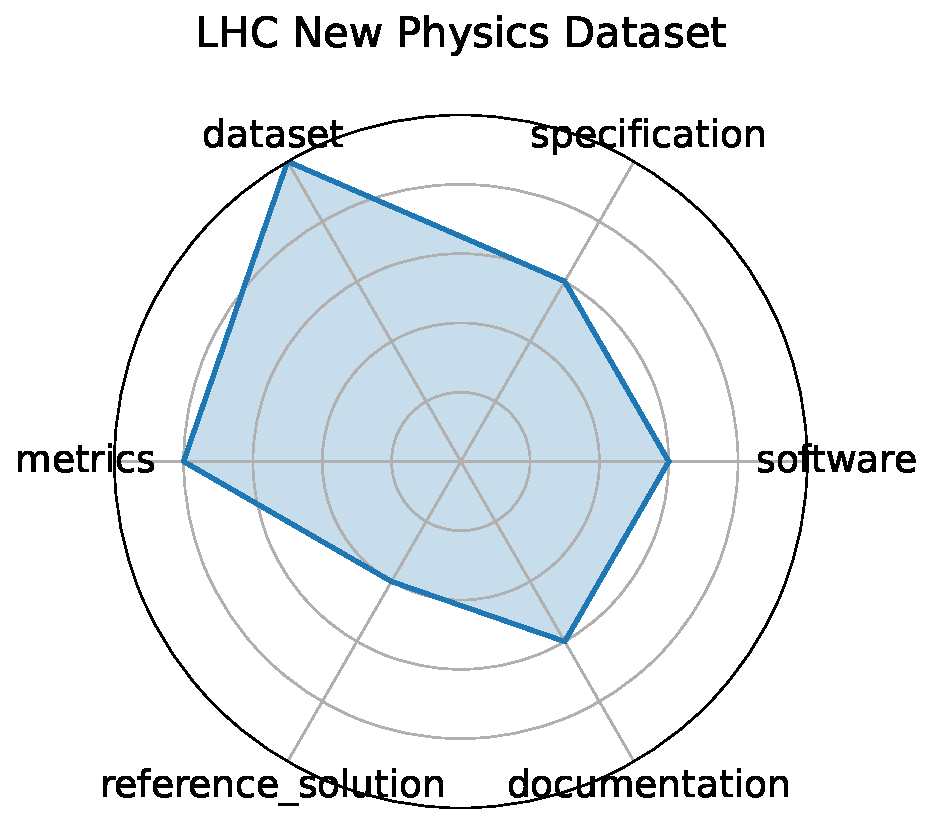
\includegraphics[width=0.15\textwidth]{lhc_new_physics_dataset_radar.pdf} & LHC New Physics Dataset & Particle Physics; Real-time Triggering & Real-time LHC event filtering for anomaly detection using proton collision data & anomaly detection, proton collision, real-time inference, event filtering, unsupervised ML & Anomaly detection, Event classification & Unsupervised signal detection under latency and bandwidth constraints & ROC-AUC, Detection efficiency & Autoencoder, Variational autoencoder, Isolation forest & \cite{https://doi.org/10.5281/zenodo.5046389}\href{https://arxiv.org/pdf/2107.02157}{$\Rightarrow$} \\ \hline
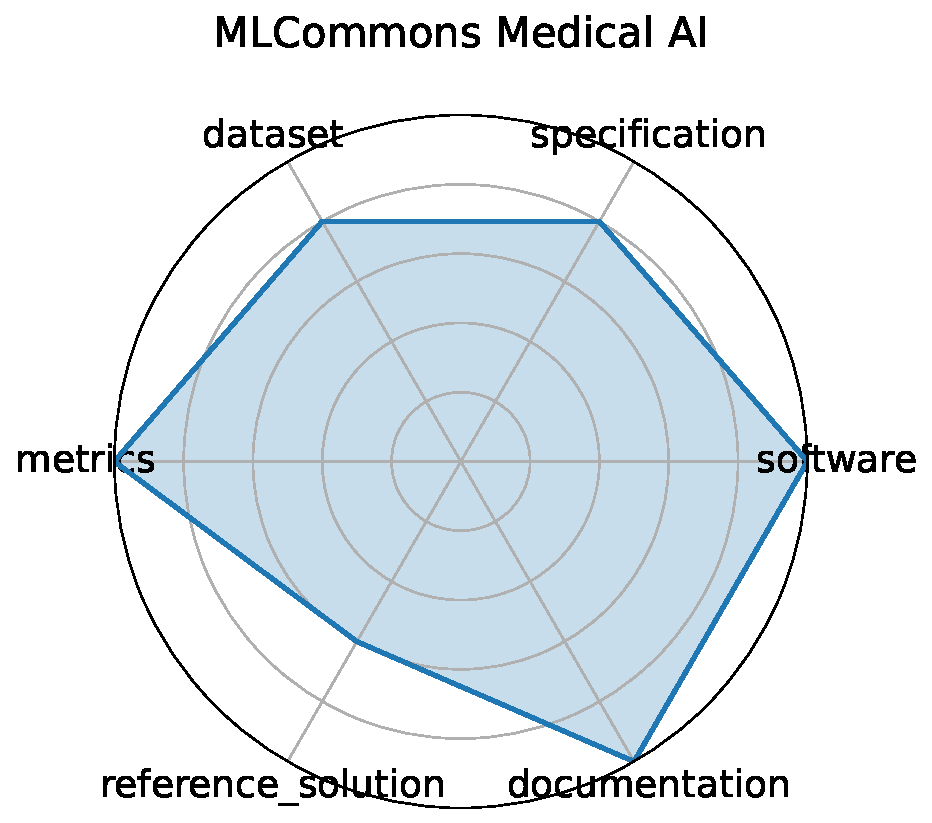
\includegraphics[width=0.15\textwidth]{mlcommons_medical_ai_radar.pdf} & MLCommons Medical AI & Healthcare; Medical AI & Federated benchmarking and evaluation of medical AI models across diverse real-world clinical data & medical AI, federated evaluation, privacy-preserving, fairness, healthcare benchmarks & Federated evaluation, Model validation & Clinical accuracy, fairness, generalizability, privacy compliance & ROC AUC, Accuracy, Fairness metrics & MedPerf-validated CNNs, GaNDLF workflows & \cite{karargyris2023federated}\href{https://github.com/mlcommons/medical}{$\Rightarrow$} \\ \hline
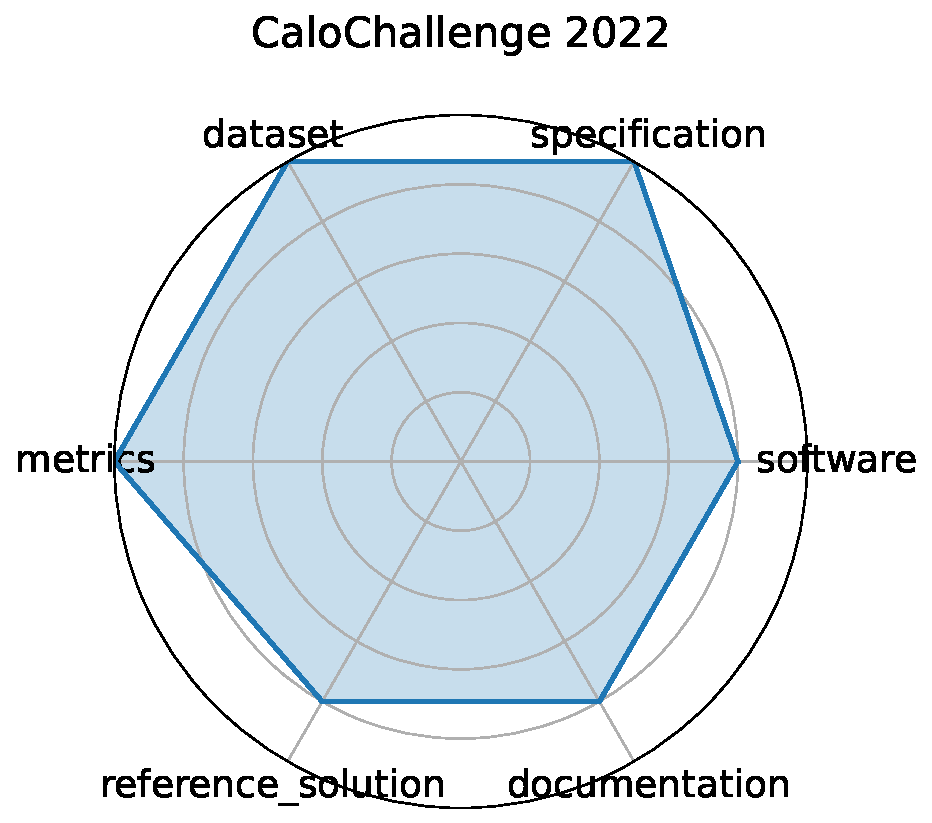
\includegraphics[width=0.15\textwidth]{calochallenge__radar.pdf} & CaloChallenge 2022 & LHC Calorimeter; Particle Physics & Fast generative-model-based calorimeter shower simulation evaluation & calorimeter simulation, generative models, surrogate modeling, LHC, fast simulation & Surrogate modeling & Simulation fidelity, speed, efficiency & Histogram similarity, Classifier AUC, Generation latency & VAE variants, GAN variants, Normalizing flows, Diffusion models & \cite{krause2024calochallenge2022communitychallenge}\href{http://arxiv.org/abs/2410.21611}{$\Rightarrow$} \\ \hline
\includegraphics[width=0.15\textwidth]{papers_with_code_sota_platform_radar.pdf} & Papers With Code (SOTA Platform) & General ML; All domains & Open platform tracking state-of-the-art results, benchmarks, and implementations across ML tasks and papers & leaderboard, benchmarking, reproducibility, open-source & Multiple (Classification, Detection, NLP, etc.) & Model performance across tasks (accuracy, F1, BLEU, etc.) & Task-specific (Accuracy, F1, BLEU, etc.) & All published models with code & \cite{pmlr-v37-blum15}\href{https://paperswithcode.com/sota}{$\Rightarrow$} \\ \hline
\includegraphics[width=0.15\textwidth]{codabench_radar.pdf} & Codabench & General ML; Multiple & Open-source platform for organizing reproducible AI benchmarks and competitions & benchmark platform, code submission, competitions, meta-benchmark & Multiple & Model reproducibility, performance across datasets & Submission count, Leaderboard ranking, Task-specific metrics & Arbitrary code submissions & \cite{xu-2022}\href{https://www.codabench.org/}{$\Rightarrow$} \\ \hline
\includegraphics[width=0.15\textwidth]{sabath_sbi-fair_radar.pdf} & Sabath (SBI-FAIR) & Systems; Metadata & FAIR metadata framework for ML-driven surrogate workflows in HPC systems & meta-benchmark, metadata, HPC, surrogate modeling & Systems benchmarking & Metadata tracking, reproducible HPC workflows & Metadata completeness, FAIR compliance & NA & \cite{luszczek2021sabath}\href{https://sbi-fair.github.io/docs/software/sabath/}{$\Rightarrow$} \\ \hline
\includegraphics[width=0.15\textwidth]{pdebench_radar.pdf} & PDEBench & CFD; Weather Modeling & Benchmark suite for ML-based surrogates solving time-dependent PDEs & PDEs, CFD, scientific ML, surrogate modeling, NeurIPS & Supervised Learning & Time-dependent PDE modeling; physical accuracy & RMSE, boundary RMSE, Fourier RMSE & FNO, U-Net, PINN, Gradient-Based inverse methods & \cite{takamoto2024pdebenchextensivebenchmarkscientific}\href{https://github.com/pdebench/PDEBench}{$\Rightarrow$} \\ \hline
\includegraphics[width=0.15\textwidth]{llm-inference-bench_radar.pdf} & LLM-Inference-Bench & LLM; HPC/inference & Hardware performance benchmarking of LLMs on AI accelerators & LLM, inference benchmarking, GPU, accelerator, throughput & Inference Benchmarking & Inference throughput, latency, hardware utilization & Token throughput (tok/s), Latency, Framework-hardware mix performance & LLaMA-2-7B, LLaMA-2-70B, Mistral-7B, Qwen-7B & \cite{10820566}\href{https://github.com/argonne-lcf/LLM-Inference-Bench}{$\Rightarrow$} \\ \hline
\includegraphics[width=0.15\textwidth]{delta_squared-dft_radar.pdf} & Delta Squared-DFT & Computational Chemistry; Materials Science & Benchmarking machine-learning corrections to DFT using Delta Squared-trained models for reaction energies & density functional theory, Delta Squared-ML correction, reaction energetics, quantum chemistry & Regression & High-accuracy energy prediction, DFT correction & Mean Absolute Error (eV), Energy ranking accuracy & Delta Squared-ML correction networks, Kernel ridge regression & \cite{khrabrov2024nabla2dftuniversalquantumchemistry}\href{https://neurips.cc/virtual/2024/poster/97788}{$\Rightarrow$} \\ \hline
\includegraphics[width=0.15\textwidth]{urban_data_layer_udl_radar.pdf} & Urban Data Layer (UDL) & Urban Computing; Data Engineering & Unified data pipeline for multi-modal urban science research & data pipeline, urban science, multi-modal, benchmark & Prediction, Classification & Multi-modal urban inference, standardization & Task-specific accuracy or RMSE & Baseline regression/classification pipelines & \cite{neurips2024_0db7f135}\href{https://neurips.cc/virtual/2024/poster/97837}{$\Rightarrow$} \\ \hline
\includegraphics[width=0.15\textwidth]{llms_for_crop_science_radar.pdf} & LLMs for Crop Science & Agricultural Science; NLP & Evaluating LLMs on crop trait QA and textual inference tasks with domain-specific prompts & crop science, prompt engineering, domain adaptation, question answering & Question Answering, Inference & Scientific knowledge, crop reasoning & Accuracy, F1 score & GPT-4, LLaMA-2-13B, T5-XXL & \cite{shen2024exploringuserretrievalintegration}\href{https://neurips.cc/virtual/2024/poster/97570}{$\Rightarrow$} \\ \hline
\includegraphics[width=0.15\textwidth]{dune_radar.pdf} & DUNE & Particle Physics & Real-time ML for DUNE DAQ time-series data & DUNE, time-series, real-time, trigger & Trigger selection, Time-series anomaly detection & Low-latency event detection & Detection efficiency, Latency & CNN, LSTM (planned) & \cite{abud2021deep}\href{https://indico.fnal.gov/event/66520/contributions/301423/attachments/182439/250508/fast\_ml\_dunedaq\_sonic\_10\_15\_24.pdf}{$\Rightarrow$} \\ \hline
\includegraphics[width=0.15\textwidth]{massspecgym_radar.pdf} & MassSpecGym & Cheminformatics; Molecular Discovery & Benchmark suite for discovery and identification of molecules via MS/MS & mass spectrometry, molecular structure, de novo generation, retrieval, dataset & De novo generation, Retrieval, Simulation & Molecular identification and generation from spectral data & Structure accuracy, Retrieval precision, Simulation MSE & Graph-based generative models, Retrieval baselines & \cite{neurips2024_c6c31413}\href{https://neurips.cc/virtual/2024/poster/97823}{$\Rightarrow$} \\ \hline
\includegraphics[width=0.15\textwidth]{hdr_ml_anomaly_challenge_gravitational_waves_radar.pdf} & HDR ML Anomaly Challenge (Gravitational Waves) & Astrophysics; Time-series & Detecting anomalous gravitational-wave signals from LIGO/Virgo datasets & anomaly detection, gravitational waves, astrophysics, time-series & Anomaly detection & Novel event detection in physical signals & ROC-AUC, Precision/Recall & Deep latent CNNs, Autoencoders & \cite{campolongo2025buildingmachinelearningchallenges}\href{https://www.codabench.org/competitions/2626/}{$\Rightarrow$} \\ \hline
\includegraphics[width=0.15\textwidth]{hdr_ml_anomaly_challenge_butterfly_radar.pdf} & HDR ML Anomaly Challenge (Butterfly) & Genomics; Image/CV & Detecting hybrid butterflies via image anomaly detection in genomic-informed dataset & anomaly detection, computer vision, genomics, butterfly hybrids & Anomaly detection & Hybrid detection in biological systems & Classification accuracy, F1 score & CNN-based detectors & \cite{campolongo2025buildingmachinelearningchallenges2}\href{https://www.codabench.org/competitions/3764/}{$\Rightarrow$} \\ \hline
\includegraphics[width=0.15\textwidth]{hdr_ml_anomaly_challenge_sea_level_rise_radar.pdf} & HDR ML Anomaly Challenge (Sea Level Rise) & Climate Science; Time-series, Image/CV & Detecting anomalous sea-level rise and flooding events via time-series and satellite imagery & anomaly detection, climate science, sea-level rise, time-series, remote sensing & Anomaly detection & Detection of environmental anomalies & ROC-AUC, Precision/Recall & CNNs, RNNs, Transformers & \cite{campolongo2025buildingmachinelearningchallenges3}\href{https://www.codabench.org/competitions/3223/}{$\Rightarrow$} \\ \hline
\includegraphics[width=0.15\textwidth]{single_qubit_readout_on_qick_system_radar.pdf} & Single Qubit Readout on QICK System & Quantum Computing & Real-time single-qubit state classification using FPGA firmware & qubit readout, hls4ml, FPGA, QICK & Classification & Single-shot fidelity, inference latency & Accuracy, Latency & hls4ml quantized NN & \cite{diguglielmo2025endtoendworkflowmachinelearningbased}\href{https://github.com/fastmachinelearning/ml-quantum-readout}{$\Rightarrow$} \\ \hline
\includegraphics[width=0.15\textwidth]{gpqa_a_graduate-level_google-proof_question_and_answer_benchmark_radar.pdf} & GPQA: A Graduate-Level Google-Proof Question and Answer Benchmark & Science (Biology, Physics, Chemistry) & Graduate-level, expert-validated multiple-choice questions hard even with web access & Google-proof, multiple-choice, expert reasoning, science QA & Multiple choice & Scientific reasoning, knowledge probing & Accuracy & GPT-4 baseline & \cite{rein2023gpqagraduatelevelgoogleproofqa2}\href{https://arxiv.org/abs/2311.12022}{$\Rightarrow$} \\ \hline
\includegraphics[width=0.15\textwidth]{seafloorai_radar.pdf} & SeafloorAI & Marine Science; Vision-Language & Large-scale vision-language dataset for seafloor mapping and geological classification & sonar imagery, vision-language, seafloor mapping, segmentation, QA & Image segmentation, Vision-language QA & Geospatial understanding, multimodal reasoning & Segmentation pixel accuracy, QA accuracy & SegFormer, ViLT-style multimodal models & \cite{nguyen2024seafloor}\href{https://neurips.cc/virtual/2024/poster/97432}{$\Rightarrow$} \\ \hline
\includegraphics[width=0.15\textwidth]{supercond_radar.pdf} & SuperCon3D & Materials Science; Superconductivity & Dataset and models for predicting and generating high-Tc superconductors using 3D crystal structures & superconductivity, crystal structures, equivariant GNN, generative models & Regression (Tc prediction), Generative modeling & Structure-to-property prediction, structure generation & MAE (Tc), Validity of generated structures & SODNet, DiffCSP-SC & \cite{neurips2024_c4e3b55e}\href{https://neurips.cc/virtual/2024/poster/97553}{$\Rightarrow$} \\ \hline
\includegraphics[width=0.15\textwidth]{gess_radar.pdf} & GeSS & Scientific ML; Geometric Deep Learning & Benchmark suite evaluating geometric deep learning models under real-world distribution shifts & geometric deep learning, distribution shift, OOD robustness, scientific applications & Classification, Regression & OOD performance in scientific settings & Accuracy, RMSE, OOD robustness delta & GCN, EGNN, DimeNet++ & \cite{neurips2024_a8063075}\href{https://neurips.cc/virtual/2024/poster/97816}{$\Rightarrow$} \\ \hline
\includegraphics[width=0.15\textwidth]{vocal_call_locator_vcl_radar.pdf} & Vocal Call Locator (VCL) & Neuroscience; Bioacoustics & Benchmarking sound-source localization of rodent vocalizations from multi-channel audio & source localization, bioacoustics, time-series, SSL & Sound source localization & Source localization accuracy in bioacoustic settings & Localization error (cm), Recall/Precision & CNN-based SSL models & \cite{neurips2024_c00d37d6}\href{https://neurips.cc/virtual/2024/poster/97470}{$\Rightarrow$} \\ \hline
\includegraphics[width=0.15\textwidth]{spiqa_llm_radar.pdf} & SPIQA (LLM) & Multimodal Scientific QA; Computer Vision & Evaluating LLMs on image-based scientific paper figure QA tasks (LLM Adapter performance) & multimodal QA, scientific figures, image+text, chain-of-thought prompting & Multimodal QA & Visual reasoning, scientific figure understanding & Accuracy, F1 score & LLaVA, MiniGPT-4, Owl-LLM adapter variants & \cite{pramanick2025spiqadatasetmultimodalquestion}\href{https://neurips.cc/virtual/2024/poster/97575}{$\Rightarrow$} \\ \hline
\includegraphics[width=0.15\textwidth]{the_well_radar.pdf} & The Well & biological systems, fluid dynamics, acoustic scattering, astrophysical MHD & Foundation model + surrogate dataset spanning 16 physical simulation domains & surrogate modeling, foundation model, physics simulations, spatiotemporal dynamics & Supervised Learning & Surrogate modeling, physics-based prediction & Dataset size, Domain breadth & FNO baselines, U-Net baselines & \cite{neurips2024_4f9a5acd}\href{https://polymathic-ai.org/the\_well/}{$\Rightarrow$} \\ \hline
\end{longtable}
}

\end{landscape}


\clearpage


\section{Radar Chart Table}


\begin{figure}[ht!]
\centering
\includegraphics[width=0.1900\textwidth]{images/mmlu_massive_multitask_language_understanding_radar.pdf}
\includegraphics[width=0.1900\textwidth]{images/commonsenseqa_radar.pdf}
\includegraphics[width=0.1900\textwidth]{images/winogrande_radar.pdf}
\includegraphics[width=0.1900\textwidth]{images/big-bench_beyond_the_imitation_game_benchmark_radar.pdf}
\includegraphics[width=0.1900\textwidth]{images/climatelearn_radar.pdf}
\\[1ex]
\includegraphics[width=0.1900\textwidth]{images/cfdbench_fluid_dynamics_radar.pdf}
\includegraphics[width=0.1900\textwidth]{images/satimgnet_radar.pdf}
\includegraphics[width=0.1900\textwidth]{images/quantum_computing_benchmarks_qml_radar.pdf}
\includegraphics[width=0.1900\textwidth]{images/ocp_open_catalyst_project_radar.pdf}
\includegraphics[width=0.1900\textwidth]{images/medqa_radar.pdf}
\\[1ex]
\includegraphics[width=0.1900\textwidth]{images/materials_project_radar.pdf}
\includegraphics[width=0.1900\textwidth]{images/gpqa_diamond_radar.pdf}
\includegraphics[width=0.1900\textwidth]{images/arc-challenge_advanced_reasoning_challenge_radar.pdf}
\includegraphics[width=0.1900\textwidth]{images/humanitys_last_exam_radar.pdf}
\includegraphics[width=0.1900\textwidth]{images/frontiermath_radar.pdf}
\\[1ex]
\includegraphics[width=0.1900\textwidth]{images/scicode_radar.pdf}
\includegraphics[width=0.1900\textwidth]{images/aime_american_invitational_mathematics_examination_radar.pdf}
\includegraphics[width=0.1900\textwidth]{images/math-_radar.pdf}
\includegraphics[width=0.1900\textwidth]{images/curie_scientific_long-context_understanding_reasoning_and_information_extraction_radar.pdf}
\includegraphics[width=0.1900\textwidth]{images/feabench_finite_element_analysis_benchmark_radar.pdf}
\\[1ex]
\includegraphics[width=0.1900\textwidth]{images/spiqa_scientific_paper_image_question_answering_radar.pdf}
\includegraphics[width=0.1900\textwidth]{images/baisbench_biological_ai_scientist_benchmark_radar.pdf}
\includegraphics[width=0.1900\textwidth]{images/molgen_radar.pdf}
\includegraphics[width=0.1900\textwidth]{images/open_graph_benchmark_ogb_-_biology_radar.pdf}
\includegraphics[width=0.1900\textwidth]{images/jarvis-leaderboard_radar.pdf}
\\[1ex]
\caption{Radar chart overview (page 1)}
\end{figure}


\clearpage

\begin{figure}[ht!]
\centering
\includegraphics[width=0.1900\textwidth]{images/nixtla_neural_forecast_timegpt_radar.pdf}
\includegraphics[width=0.1900\textwidth]{images/nixtla_neural_forecast_nhits_radar.pdf}
\includegraphics[width=0.1900\textwidth]{images/nixtla_neural_forecast_timellm_radar.pdf}
\includegraphics[width=0.1900\textwidth]{images/nixtla_neuralforecast_radar.pdf}
\includegraphics[width=0.1900\textwidth]{images/vllm_performance_dashboard_radar.pdf}
\\[1ex]
\includegraphics[width=0.1900\textwidth]{images/vllm_inference_and_serving_engine_radar.pdf}
\includegraphics[width=0.1900\textwidth]{images/sglang_framework_radar.pdf}
\includegraphics[width=0.1900\textwidth]{images/jet_classification_radar.pdf}
\includegraphics[width=0.1900\textwidth]{images/irregular_sensor_data_compression_radar.pdf}
\includegraphics[width=0.1900\textwidth]{images/beam_control_radar.pdf}
\\[1ex]
\includegraphics[width=0.1900\textwidth]{images/ultrafast_jet_classification_at_the_hl-lhc_radar.pdf}
\includegraphics[width=0.1900\textwidth]{images/quench_detection_radar.pdf}
\includegraphics[width=0.1900\textwidth]{images/intelligent_experiments_through_real-time_ai_radar.pdf}
\includegraphics[width=0.1900\textwidth]{images/neural_architecture_codesign_for_fast_physics_applications_radar.pdf}
\includegraphics[width=0.1900\textwidth]{images/smart_pixels_for_lhc_radar.pdf}
\\[1ex]
\includegraphics[width=0.1900\textwidth]{images/hedm_braggnn_radar.pdf}
\includegraphics[width=0.1900\textwidth]{images/d-stem_radar.pdf}
\includegraphics[width=0.1900\textwidth]{images/in-situ_high-speed_computer_vision_radar.pdf}
\includegraphics[width=0.1900\textwidth]{images/benchcouncil_aibench_radar.pdf}
\includegraphics[width=0.1900\textwidth]{images/benchcouncil_bigdatabench_radar.pdf}
\\[1ex]
\includegraphics[width=0.1900\textwidth]{images/mlperf_hpc_radar.pdf}
\includegraphics[width=0.1900\textwidth]{images/mlcommons_science_radar.pdf}
\includegraphics[width=0.1900\textwidth]{images/lhc_new_physics_dataset_radar.pdf}
\includegraphics[width=0.1900\textwidth]{images/mlcommons_medical_ai_radar.pdf}
\includegraphics[width=0.1900\textwidth]{images/calochallenge__radar.pdf}
\\[1ex]
\caption{Radar chart overview (page 2)}
\end{figure}


\clearpage

\begin{figure}[ht!]
\centering
\includegraphics[width=0.1900\textwidth]{images/papers_with_code_sota_platform_radar.pdf}
\includegraphics[width=0.1900\textwidth]{images/codabench_radar.pdf}
\includegraphics[width=0.1900\textwidth]{images/sabath_sbi-fair_radar.pdf}
\includegraphics[width=0.1900\textwidth]{images/pdebench_radar.pdf}
\includegraphics[width=0.1900\textwidth]{images/llm-inference-bench_radar.pdf}
\\[1ex]
\includegraphics[width=0.1900\textwidth]{images/delta_squared-dft_radar.pdf}
\includegraphics[width=0.1900\textwidth]{images/urban_data_layer_udl_radar.pdf}
\includegraphics[width=0.1900\textwidth]{images/llms_for_crop_science_radar.pdf}
\includegraphics[width=0.1900\textwidth]{images/dune_radar.pdf}
\includegraphics[width=0.1900\textwidth]{images/massspecgym_radar.pdf}
\\[1ex]
\includegraphics[width=0.1900\textwidth]{images/hdr_ml_anomaly_challenge_gravitational_waves_radar.pdf}
\includegraphics[width=0.1900\textwidth]{images/hdr_ml_anomaly_challenge_butterfly_radar.pdf}
\includegraphics[width=0.1900\textwidth]{images/hdr_ml_anomaly_challenge_sea_level_rise_radar.pdf}
\includegraphics[width=0.1900\textwidth]{images/single_qubit_readout_on_qick_system_radar.pdf}
\includegraphics[width=0.1900\textwidth]{images/gpqa_a_graduate-level_google-proof_question_and_answer_benchmark_radar.pdf}
\\[1ex]
\includegraphics[width=0.1900\textwidth]{images/seafloorai_radar.pdf}
\includegraphics[width=0.1900\textwidth]{images/supercond_radar.pdf}
\includegraphics[width=0.1900\textwidth]{images/gess_radar.pdf}
\includegraphics[width=0.1900\textwidth]{images/vocal_call_locator_vcl_radar.pdf}
\includegraphics[width=0.1900\textwidth]{images/spiqa_llm_radar.pdf}
\\[1ex]
\includegraphics[width=0.1900\textwidth]{images/the_well_radar.pdf}
\caption{Radar chart overview (page 3)}
\end{figure}



\clearpage


\section{Benchmark Details}

\subsection{MMLU (Massive Multitask Language Understanding)}
{{\footnotesize
\noindent Measuring Massive Multitask Language Understanding (MMLU) is a benchmark of 57 
multiple-choice tasks covering elementary mathematics, US history, computer science, 
law, and more, designed to evaluate a model's breadth and depth of knowledge in 
zero-shot and few-shot settings.


\begin{description}[labelwidth=4cm, labelsep=1em, leftmargin=4cm, itemsep=0.1em, parsep=0em]
  \item[date:] 2020-09-07
  \item[version:] 1
  \item[last\_updated:] 2020-09-07
  \item[expired:] false
  \item[valid:] yes
  \item[valid\_date:] 2025-07-28
  \item[url:] \href{https://paperswithcode.com/dataset/mmlu}{https://paperswithcode.com/dataset/mmlu}
  \item[doi:] 10.48550/arXiv.2009.03300
  \item[domain:] Multidomain
  \item[focus:] Academic knowledge and reasoning across 57 subjects
  \item[keywords:]
    - multitask
    - multiple-choice
    - zero-shot
    - few-shot
    - knowledge probing
  \item[licensing:] MIT License
  \item[task\_types:]
    - Multiple choice
  \item[ai\_capability\_measured:]
    - General reasoning, subject-matter understanding
  \item[metrics:]
    - Accuracy
  \item[models:]
    - GPT-4o
    - Gemini 1.5 Pro
    - o1
    - DeepSeek-R1
  \item[ml\_motif:]
    - General knowledge
  \item[type:] Benchmark
  \item[ml\_task:]
    - Supervised Learning
  \item[solutions:] 1
  \item[notes:] Good
  \item[contact.name:] Dan Hendrycks
  \item[contact.email:] dan (at) safe.ai
  \item[datasets.links.name:] Papers with Code datasets
  \item[datasets.links.url:] \href{https://github.com/paperswithcode/paperswithcode-data}{https://github.com/paperswithcode/paperswithcode-data}
  \item[results.links.name:] Chinchilla
  \item[results.links.url:] \href{https://arxiv.org/abs/2203.15556}{https://arxiv.org/abs/2203.15556}
  \item[fair.reproducible:] True
  \item[fair.benchmark\_ready:] True
  \item[id:] mmlu\_massive\_multitask\_language\_understanding
  \item[Citations:] \cite{hendrycks2021measuring}
\end{description}

{\bf Ratings:} ~ \\

\begin{tabular}{p{0.15\textwidth} p{0.07\textwidth} p{0.7\textwidth}}
\hline
Rating & Value & Reason \\
\hline
dataset & 5 & Meets all FAIR principles and properly versioned.
 \\
documentation & 5 & Well-explained in a provided paper.
 \\
metrics & 5 & Fully defined, represents a solution's performance.
 \\
reference\_solution & 2 & Reference models are available (i.e. GPT-3), but are not trainable or publicly documented
 \\
software & 0 & No instructions to download or run data given on the site
 \\
specification & 4 & No system constraints
 \\
\hline
\end{tabular}

\includegraphics[width=0.2\textwidth]{mmlu_massive_multitask_language_understanding_radar.pdf}
}}
\clearpage
\subsection{CommonSenseQA}
{{\footnotesize
\noindent CommonsenseQA is a challenging multiple-choice QA dataset built from ConceptNet,
requiring models to apply commonsense knowledge to select the correct answer 
among five choices.


\begin{description}[labelwidth=4cm, labelsep=1em, leftmargin=4cm, itemsep=0.1em, parsep=0em]
  \item[date:] 2019-11-20
  \item[version:] 1
  \item[last\_updated:] 2019-11-20
  \item[expired:] false
  \item[valid:] yes
  \item[valid\_date:] 2019-11-20
  \item[url:] \href{https://paperswithcode.com/paper/commonsenseqa-a-question-answering-challenge}{https://paperswithcode.com/paper/commonsenseqa-a-question-answering-challenge}
  \item[doi:] 10.48550/arXiv.1811.00937
  \item[domain:] NLP; Commonsense
  \item[focus:] Commonsense question answering
  \item[keywords:]
    - ConceptNet
    - multiple-choice
    - adversarial
  \item[licensing:] MIT
  \item[task\_types:]
    - Multiple choice
  \item[ai\_capability\_measured:]
    - Commonsense reasoning and knowledge integration
  \item[metrics:]
    - Accuracy
  \item[models:]
    - BERT-large
    - RoBERTa
    - GPT-3
  \item[ml\_motif:]
    - Commonsense question answering
  \item[type:] Benchmark
  \item[ml\_task:]
    - Supervised Learning
  \item[solutions:] 2
  \item[notes:] Baseline 56\%, human 89\%
  \item[contact.name:] Alon Talmor, Jonathan Herzig, Nicholas Lourie, Jonathan Berant
  \item[contact.email:] Unknown
  \item[datasets.links.name:] CommonsenseQA Dataset (Hugging Face)
  \item[datasets.links.url:] \href{https://huggingface.co/datasets/commonsense\_qa}{https://huggingface.co/datasets/commonsense\_qa}
  \item[results.links.name:] Papers With Code Leaderboard for CommonsenseQA
  \item[results.links.url:] \href{https://paperswithcode.com/dataset/commonsenseqa}{https://paperswithcode.com/dataset/commonsenseqa}
  \item[fair.reproducible:] True
  \item[fair.benchmark\_ready:] True
  \item[id:] commonsenseqa
  \item[Citations:] \cite{talmor2019commonsenseqaquestionansweringchallenge}
\end{description}

{\bf Ratings:} ~ \\

\begin{tabular}{p{0.15\textwidth} p{0.07\textwidth} p{0.7\textwidth}}
\hline
Rating & Value & Reason \\
\hline
dataset & 5 & Public, versioned, and FAIR-compliant; includes metadata, splits, and licensing; well-integrated with HuggingFace and other ML libraries.
 \\
documentation & 5 & Given in paper.
 \\
metrics & 5 & Accuracy is a simple, reproducible metric aligned with task goals; no ambiguity in evaluation.
 \\
reference\_solution & 4 & Several baseline models (e.g., BERT, RoBERTa) are reported with scores; implementations exist in public repos, but not run with hardware constraints
 \\
software & 5 & All code given on Github site
 \\
specification & 4 & Task and format (multiple-choice QA with 5 options) are clearly defined; grounded in ConceptNet with consistent structure, though no hardware/system constraints are specified.
 \\
\hline
\end{tabular}

\includegraphics[width=0.2\textwidth]{commonsenseqa_radar.pdf}
}}
\clearpage
\subsection{Winogrande}
{{\footnotesize
\noindent WinoGrande is a large-scale adversarial dataset of 44,000 Winograd Schema-style 
questions with reduced bias using AFLite, serving as both a benchmark and transfer 
learning resource.


\begin{description}[labelwidth=4cm, labelsep=1em, leftmargin=4cm, itemsep=0.1em, parsep=0em]
  \item[date:] 2019-07-24
  \item[version:] 1
  \item[last\_updated:] 2019-07-24
  \item[expired:] false
  \item[valid:] yes
  \item[valid\_date:] 2019-07-24
  \item[url:] \href{https://leaderboard.allenai.org/winogrande/submissions/public}{https://leaderboard.allenai.org/winogrande/submissions/public}
  \item[doi:] 10.48550/arXiv.1907.10641
  \item[domain:] NLP; Commonsense
  \item[focus:] Winograd Schema-style pronoun resolution
  \item[keywords:]
    - adversarial
    - pronoun resolution
  \item[licensing:] CC-BY
  \item[task\_types:]
    - Pronoun resolution
  \item[ai\_capability\_measured:]
    - Robust commonsense reasoning
  \item[metrics:]
    - Accuracy
    - AUC
  \item[models:]
    - RoBERTa
    - BERT
    - GPT-2
  \item[ml\_motif:]
    - Commonsense reasoning
  \item[type:] Benchmark
  \item[ml\_task:]
    - Supervised Learning
  \item[solutions:] 2
  \item[notes:] Human \textasciitilde{}94\%
  \item[contact.name:] Keisuke Sakaguchi
  \item[contact.email:] keisukes@allenai.org
  \item[datasets.links.name:] Hugging Face / AllenAI
  \item[datasets.links.url:] \href{https://huggingface.co/datasets/allenai/winogrande}{https://huggingface.co/datasets/allenai/winogrande}
  \item[results.links.name:] Papers With Code leaderboard
  \item[results.links.url:] \href{https://paperswithcode.com/dataset/winogrande}{https://paperswithcode.com/dataset/winogrande}
  \item[fair.reproducible:] True
  \item[fair.benchmark\_ready:] True
  \item[id:] winogrande
  \item[Citations:] \cite{sakaguchi2019winograndeadversarialwinogradschema}
\end{description}

{\bf Ratings:} ~ \\

\begin{tabular}{p{0.15\textwidth} p{0.07\textwidth} p{0.7\textwidth}}
\hline
Rating & Value & Reason \\
\hline
dataset & 5 & Public, versioned, and FAIR-compliant with AFLite-generated splits to reduce annotation artifacts; hosted by AllenAI with good metadata.
 \\
documentation & 5 & Dataset page and paper provide sufficient detail
 \\
metrics & 5 & Accuracy and AUC are quantitative and well-aligned with disambiguation goals; standardized across evaluations.
 \\
reference\_solution & 4 & Baseline results available, requiring users to submit their methods along with their submissions. Constraints are not required in submissions.
 \\
software & 0 & No template code provided
 \\
specification & 5 & Task (pronoun/coreference resolution) is clearly defined in Winograd Schema style, with consistent input/output format; no system constraints included.
 \\
\hline
\end{tabular}

\includegraphics[width=0.2\textwidth]{winogrande_radar.pdf}
}}
\clearpage
\subsection{BIG-Bench (Beyond the Imitation Game Benchmark)}
{{\footnotesize
\noindent BIG-Bench is a collaborative suite of 204 tasks designed to probe LLMs' reasoning, 
knowledge, and bias across diverse domains and difficulty levels beyond simple imitation.


\begin{description}[labelwidth=4cm, labelsep=1em, leftmargin=4cm, itemsep=0.1em, parsep=0em]
  \item[date:] 2022-06-09
  \item[version:] 1
  \item[last\_updated:] 2022-06-09
  \item[expired:] false
  \item[valid:] yes
  \item[valid\_date:] 2022-06-09
  \item[url:] \href{https://github.com/google/BIG-bench}{https://github.com/google/BIG-bench}
  \item[doi:] 10.48550/arXiv.2206.04615
  \item[domain:] NLP; AI Evaluation
  \item[focus:] Diverse reasoning and generalization tasks
  \item[keywords:]
    - few-shot
    - multi-task
    - bias analysis
  \item[licensing:] Apache-2.0
  \item[task\_types:]
    - Few-shot evaluation
    - Multi-task evaluation
  \item[ai\_capability\_measured:]
    - Reasoning and generalization across diverse tasks
  \item[metrics:]
    - Accuracy
    - Task-specific metrics
  \item[models:]
    - GPT-3
    - Dense Transformers
    - Sparse Transformers
  \item[ml\_motif:]
    - LLM evaluation
  \item[type:] Benchmark
  \item[ml\_task:]
    - Supervised Learning
  \item[solutions:] Multiple, including human baselines
  \item[notes:] Human baselines included
  \item[contact.name:] Aarohi Srivastava et al.
  \item[contact.email:] bigbench@googlegroups.com
  \item[datasets.links.name:] BIG-Bench GitHub Repository (contains tasks and data)
  \item[datasets.links.url:] \href{https://github.com/google/BIG-bench/tree/main/bigbench/benchmark\_tasks}{https://github.com/google/BIG-bench/tree/main/bigbench/benchmark\_tasks}
  \item[results.links.name:] BIG-Bench GitHub Repository (results in papers and code)
  \item[results.links.url:] \href{https://github.com/google/BIG-bench}{https://github.com/google/BIG-bench}
  \item[fair.reproducible:] True
  \item[fair.benchmark\_ready:] True
  \item[id:] big-bench\_beyond\_the\_imitation\_game\_benchmark
  \item[Citations:] \cite{srivastava2023imitationgamequantifyingextrapolating}
\end{description}

{\bf Ratings:} ~ \\

\begin{tabular}{p{0.15\textwidth} p{0.07\textwidth} p{0.7\textwidth}}
\hline
Rating & Value & Reason \\
\hline
dataset & 5 & Public, versioned, and well-documented; FAIR overall
 \\
documentation & 5 & Explained in the associated paper.
 \\
metrics & 5 & Many tasks use standard quantitative metrics (accuracy, BLEU, F1). Others involve subjective ratings (e.g., Likert), which reduces cross-task comparability.
 \\
reference\_solution & 2 & Human baselines and LLM performance results are included; however, runnable reference solutions are limited and setup is not fully turnkey.
 \\
software & 4.5 & Quick start notebook provided, but instructions on how to run it are lacking.
 \\
specification & 4.5 & Tasks are diverse and clearly described; input/output formats are usually defined but vary widely, and system constraints are not standardized.
 \\
\hline
\end{tabular}

\includegraphics[width=0.2\textwidth]{big-bench_beyond_the_imitation_game_benchmark_radar.pdf}
}}
\clearpage
\subsection{ClimateLearn}
{{\footnotesize
\noindent ClimateLearn provides standardized datasets and evaluation protocols for machine 
learning models in medium-range weather and climate forecasting using ERA5 reanalysis.


\begin{description}[labelwidth=4cm, labelsep=1em, leftmargin=4cm, itemsep=0.1em, parsep=0em]
  \item[date:] 2023-07-19
  \item[version:] 1
  \item[last\_updated:] 2023-07-19
  \item[expired:] false
  \item[valid:] yes
  \item[valid\_date:] 2023-07-19
  \item[url:] \href{https://arxiv.org/abs/2307.01909}{https://arxiv.org/abs/2307.01909}
  \item[doi:] 10.48550/arXiv.2307.01909
  \item[domain:] Climate Science; Forecasting
  \item[focus:] ML for weather and climate modeling
  \item[keywords:]
    - medium-range forecasting
    - ERA5
    - data-driven
  \item[licensing:] CC-BY-4.0
  \item[task\_types:]
    - Forecasting
  \item[ai\_capability\_measured:]
    - Global weather prediction (3-5 days)
  \item[metrics:]
    - RMSE
    - Anomaly correlation
  \item[models:]
    - CNN baselines
    - ResNet variants
  \item[ml\_motif:]
    - Forecasting
    - Benchmarking
  \item[type:] Benchmark
  \item[ml\_task:]
    - Supervised Learning
  \item[solutions:] Multiple baseline models provided
  \item[notes:] Includes physical and ML baselines.
  \item[contact.name:] Jason Jewik
  \item[contact.email:] jason.jewik@ucla.edu
  \item[datasets.links.name:] ClimateLearn GitHub Repository (data loaders and processing)
  \item[datasets.links.url:] \href{https://github.com/aditya-grover/climate-learn}{https://github.com/aditya-grover/climate-learn}
  \item[results.links.name:] ClimateLearn Paper (results section)
  \item[results.links.url:] \href{https://arxiv.org/abs/2307.01909}{https://arxiv.org/abs/2307.01909}
  \item[fair.reproducible:] True
  \item[fair.benchmark\_ready:] True
  \item[id:] climatelearn
  \item[Citations:] \cite{nguyen2023climatelearnbenchmarkingmachinelearning}
\end{description}

{\bf Ratings:} ~ \\

\begin{tabular}{p{0.15\textwidth} p{0.07\textwidth} p{0.7\textwidth}}
\hline
Rating & Value & Reason \\
\hline
dataset & 5 & Provides standardized access to ERA5 and other reanalysis datasets, with ML-ready splits, metadata, and Xarray-compatible formats; versioned and fully FAIR-compliant.
 \\
documentation & 5 & Explained in the benchmark's paper. 
 \\
metrics & 5 & ACC and RMSE are standard, quantitative, and appropriate for climate forecasting; well-integrated into the benchmark, though interpretation across domains may vary.
 \\
reference\_solution & 0 & The benchmark is geared for CNN architectures, but no specific model was mentioned.
 \\
software & 5 & Quickstart notebook makes for easy usage
 \\
specification & 5 & Task framing (medium-range climate forecasting), input/output formats, and evaluation windows are clearly defined; benchmark supports both physical and learned models with detailed constraints.
 \\
\hline
\end{tabular}

\includegraphics[width=0.2\textwidth]{climatelearn_radar.pdf}
}}
\clearpage
\subsection{CFDBench (Fluid Dynamics)}
{{\footnotesize
\noindent CFDBench provides large-scale CFD data for four canonical fluid flow problems, 
assessing neural operators' ability to generalize to unseen PDE parameters and domains.


\begin{description}[labelwidth=4cm, labelsep=1em, leftmargin=4cm, itemsep=0.1em, parsep=0em]
  \item[date:] 2024-10-01
  \item[version:] 1
  \item[last\_updated:] 2024-10-01
  \item[expired:] false
  \item[valid:] yes
  \item[valid\_date:] 2024-10-01
  \item[url:] \href{https://arxiv.org/abs/2310.05963}{https://arxiv.org/abs/2310.05963}
  \item[doi:] 10.48550/arXiv.2310.05963
  \item[domain:] Fluid Dynamics; Scientific ML
  \item[focus:] Neural operator surrogate modeling
  \item[keywords:]
    - neural operators
    - CFD
    - FNO
    - DeepONet
  \item[licensing:] CC-BY-4.0
  \item[task\_types:]
    - Surrogate modeling
  \item[ai\_capability\_measured:]
    - Generalization of neural operators for PDEs
  \item[metrics:]
    - L2 error
    - MAE
  \item[models:]
    - FNO
    - DeepONet
    - U-Net
  \item[ml\_motif:]
    - Generalization
  \item[type:] Benchmark
  \item[ml\_task:]
    - Supervised Learning
  \item[solutions:] Numerous, as it's a benchmark for ML models
  \item[notes:] 302K frames across 739 cases
  \item[contact.name:] Yining Luo
  \item[contact.email:] yining.luo@mail.utoronto.ca
  \item[datasets.links.name:] unknown
  \item[datasets.links.url:] \href{unknown}{unknown}
  \item[results.links.name:] unknown
  \item[results.links.url:] \href{unknown}{unknown}
  \item[fair.reproducible:] True
  \item[fair.benchmark\_ready:] True
  \item[id:] cfdbench\_fluid\_dynamics
  \item[Citations:] \cite{luo2024cfdbenchlargescalebenchmarkmachine}
\end{description}

{\bf Ratings:} ~ \\

\begin{tabular}{p{0.15\textwidth} p{0.07\textwidth} p{0.7\textwidth}}
\hline
Rating & Value & Reason \\
\hline
dataset & 0 & Not given
 \\
documentation & 5 & Associated paper gives all necessary information.
 \\
metrics & 5 & Quantitative metrics (L2 error, MAE, relative error) are clearly defined and align with regression task objectives.
 \\
reference\_solution & 5 & Baseline models like FNO and DeepONet are implemented, hardware specified.
 \\
software & 5 & The benchmark provides Python scripts for data loading, preprocessing, and model training/evaluation
 \\
specification & 0 & Not listed
 \\
\hline
\end{tabular}

\includegraphics[width=0.2\textwidth]{cfdbench_fluid_dynamics_radar.pdf}
}}
\clearpage
\subsection{SatImgNet}
{{\footnotesize
\noindent SATIN (sometimes referred to as SatImgNet) is a multi-task metadataset of 27 satellite
imagery classification datasets evaluating zero-shot transfer of vision-language models
across diverse remote sensing tasks.


\begin{description}[labelwidth=4cm, labelsep=1em, leftmargin=4cm, itemsep=0.1em, parsep=0em]
  \item[date:] 2023-04-23
  \item[version:] 1
  \item[last\_updated:] 2023-04-23
  \item[expired:] false
  \item[valid:] yes
  \item[valid\_date:] 2023-04-23
  \item[url:] \href{https://huggingface.co/datasets/saral-ai/satimagnet}{https://huggingface.co/datasets/saral-ai/satimagnet}
  \item[doi:] 10.48550/arXiv.2304.11619
  \item[domain:] Remote Sensing
  \item[focus:] Satellite imagery classification
  \item[keywords:]
    - land-use
    - zero-shot
    - multi-task
  \item[licensing:] CC-BY-4.0
  \item[task\_types:]
    - Image classification
  \item[ai\_capability\_measured:]
    - Zero-shot land-use classification
  \item[metrics:]
    - Accuracy
  \item[models:]
    - CLIP
    - BLIP
    - ALBEF
  \item[ml\_motif:]
    - Transfer Learning
  \item[type:] Benchmark
  \item[ml\_task:]
    - Supervised Learning
  \item[solutions:] Numerous, evaluated via leaderboard
  \item[notes:] Public leaderboard available
  \item[contact.name:] Jonathan Roberts
  \item[contact.email:] j.roberts@cs.ox.ac.uk
  \item[datasets.links.name:] SatImgNet on Hugging Face
  \item[datasets.links.url:] \href{https://huggingface.co/datasets/saral-ai/satimagnet}{https://huggingface.co/datasets/saral-ai/satimagnet}
  \item[results.links.name:] SatImgNet Leaderboard
  \item[results.links.url:] \href{https://huggingface.co/spaces/saral-ai/satin-leaderboard}{https://huggingface.co/spaces/saral-ai/satin-leaderboard}
  \item[fair.reproducible:] True
  \item[fair.benchmark\_ready:] True
  \item[id:] satimgnet
  \item[Citations:] \cite{roberts2023satin}
\end{description}

{\bf Ratings:} ~ \\

\begin{tabular}{p{0.15\textwidth} p{0.07\textwidth} p{0.7\textwidth}}
\hline
Rating & Value & Reason \\
\hline
dataset & 5 & Hosted on Hugging Face, versioned, FAIR-compliant with rich metadata; covers many well-known remote sensing datasets unified under one metadataset, though documentation depth varies slightly across tasks.
 \\
documentation & 5 & Paper provides all required information
 \\
metrics & 5 & Accuracy of classification is an appropriate metric
 \\
reference\_solution & 4 & Baselines like CLIP, BLIP, ALBEF evaluated in the paper; no constraints specified
 \\
software & 0 & No scripts or environment information provided
 \\
specification & 4 & Tasks (image classification across 27 satellite datasets) are clearly defined with multi-task and zero-shot framing; input/output structure is mostly standard but some task-specific nuances require interpretation.
 \\
\hline
\end{tabular}

\includegraphics[width=0.2\textwidth]{satimgnet_radar.pdf}
}}
\clearpage
\subsection{Quantum Computing Benchmarks (QML)}
{{\footnotesize
\noindent A suite of benchmarks evaluating quantum hardware and algorithms on tasks such as state 
preparation, circuit optimization, and error correction across multiple platforms.


\begin{description}[labelwidth=4cm, labelsep=1em, leftmargin=4cm, itemsep=0.1em, parsep=0em]
  \item[date:] 2022-02-22
  \item[version:] 1
  \item[last\_updated:] 2022-02-22
  \item[expired:] false
  \item[valid:] yes
  \item[valid\_date:] 2022-02-22
  \item[url:] \href{https://github.com/XanaduAI/qml-benchmarks}{https://github.com/XanaduAI/qml-benchmarks}
  \item[doi:] 10.48550/arXiv.2307.03901
  \item[domain:] Quantum Computing
  \item[focus:] Quantum algorithm performance evaluation
  \item[keywords:]
    - quantum circuits
    - state preparation
    - error correction
  \item[licensing:] Apache-2.0
  \item[task\_types:]
    - Circuit benchmarking
    - State classification
  \item[ai\_capability\_measured:]
    - Quantum algorithm performance and fidelity
  \item[metrics:]
    - Fidelity
    - Success probability
  \item[models:]
    - IBM Q
    - IonQ
    - AQT@LBNL
  \item[ml\_motif:]
    - Performance Evaluation
  \item[type:] Benchmark
  \item[ml\_task:]
    - Supervised Learning
  \item[solutions:] Varies per benchmark
  \item[notes:] Hardware-agnostic, application-level metrics. The citation may not be correct.
  \item[contact.name:] Xanadu AI
  \item[contact.email:] support@xanadu.ai
  \item[datasets.links.name:] PennyLane QML Benchmarks Datasets
  \item[datasets.links.url:] \href{https://pennylane.ai/datasets/collection/qml-benchmarks}{https://pennylane.ai/datasets/collection/qml-benchmarks}
  \item[results.links.name:] QML Benchmarks GitHub Repository (Results section)
  \item[results.links.url:] \href{https://github.com/XanaduAI/qml-benchmarks\#results-and-leaderboards}{https://github.com/XanaduAI/qml-benchmarks\#results-and-leaderboards}
  \item[fair.reproducible:] True
  \item[fair.benchmark\_ready:] True
  \item[id:] quantum\_computing\_benchmarks\_qml
  \item[Citations:] \cite{kiwit2023}
\end{description}

{\bf Ratings:} ~ \\

\begin{tabular}{p{0.15\textwidth} p{0.07\textwidth} p{0.7\textwidth}}
\hline
Rating & Value & Reason \\
\hline
dataset & 4 & Datasets are accessible, but not split.
 \\
documentation & 1 & Only the task is defined. 
 \\
metrics & 3 & Partially defined, somewhat inferrable metrics. Unknown whether a system's performance is captured.
 \\
reference\_solution & 0 & Not provided
 \\
software & 4 & Run instructions exist, but are not easy to follow
 \\
specification & 3 & No system constraints. Task clarity and dataset format are not clearly specified.
 \\
\hline
\end{tabular}

\includegraphics[width=0.2\textwidth]{quantum_computing_benchmarks_qml_radar.pdf}
}}
\clearpage
\subsection{OCP (Open Catalyst Project)}
{{\footnotesize
\noindent The Open Catalyst Project (OC20 and OC22) provides DFT-calculated catalyst-adsorbate 
relaxation datasets, challenging ML models to predict energies and forces for 
renewable energy applications.


\begin{description}[labelwidth=4cm, labelsep=1em, leftmargin=4cm, itemsep=0.1em, parsep=0em]
  \item[date:] 2020-10-20
  \item[version:] 1
  \item[last\_updated:] 2020-10-20
  \item[expired:] false
  \item[valid:] yes
  \item[valid\_date:] 2020-10-20
  \item[url:] \href{https://opencatalystproject.org/}{https://opencatalystproject.org/}
  \item[doi:] unknown
  \item[domain:]
    - Chemistry
    - Materials Science
  \item[focus:] Catalyst adsorption energy prediction
  \item[keywords:]
    - DFT relaxations
    - adsorption energy
    - graph neural networks
  \item[licensing:] OCP Terms of Use
  \item[task\_types:]
    - Energy prediction
    - Force prediction
  \item[ai\_capability\_measured:]
    - Prediction of adsorption energies and forces
  \item[metrics:]
    - MAE (energy)
    - MAE (force)
  \item[models:]
    - CGCNN
    - SchNet
    - DimeNet++
    - GemNet-OC
  \item[ml\_motif:]
    - Regression
  \item[type:] Benchmark
  \item[ml\_task:]
    - Supervised Learning
  \item[solutions:] 0
  \item[notes:] Public leaderboards; active community development
  \item[contact.name:] unknown
  \item[contact.email:] unknown
  \item[datasets.links.name:] OCP Dataset
  \item[datasets.links.url:] \href{https://fair-chem.github.io/catalysts/datasets/summary}{https://fair-chem.github.io/catalysts/datasets/summary}
  \item[results.links.name:] OCP Pretrained Models
  \item[results.links.url:] \href{https://fair-chem.github.io/catalysts/models.html}{https://fair-chem.github.io/catalysts/models.html}
  \item[fair.reproducible:] Yes
  \item[fair.benchmark\_ready:] Yes
  \item[id:] ocp\_open\_catalyst\_project
  \item[Citations:] \cite{chanussot2021oc20}, \cite{tran2023oc22}, \cite{doi:10.1021/acscatal.0c04525}, \cite{tran2023b}
\end{description}

{\bf Ratings:} ~ \\

\begin{tabular}{p{0.15\textwidth} p{0.07\textwidth} p{0.7\textwidth}}
\hline
Rating & Value & Reason \\
\hline
dataset & 5 & Fully FAIR- OC20, per-adsorbate trajectories, and OC22 are versioned; datasets come with standardized splits, metadata, and are downloadable.
 \\
documentation & 1 & Paper exists, but content is behind a paywall.
 \\
metrics & 5 & MAE (energy and force) are standard and reproducible.
 \\
reference\_solution & 4 & Multiple baselines (GemNet-OC, DimeNet++, etc.) implemented and evaluated. No hardware listed.
 \\
software & 5 & Data provided in Github links
 \\
specification & 5 & Tasks (energy and force prediction) are clearly defined with explicit I/O specifications, constraints, and physical relevance for renewable energy.
 \\
\hline
\end{tabular}

\includegraphics[width=0.2\textwidth]{ocp_open_catalyst_project_radar.pdf}
}}
\clearpage
\subsection{MedQA}
{{\footnotesize
\noindent MedQA is a large-scale multiple-choice dataset drawn from professional medical
board exams (e.g., USMLE), testing AI systems on diagnostic and medical knowledge 
questions in English and Chinese.


\begin{description}[labelwidth=4cm, labelsep=1em, leftmargin=4cm, itemsep=0.1em, parsep=0em]
  \item[date:] 2020-09-28
  \item[version:] 1
  \item[last\_updated:] 2020-09-28
  \item[expired:] false
  \item[valid:] yes
  \item[valid\_date:] 2020-09-28
  \item[url:] \href{https://arxiv.org/abs/2009.13081}{https://arxiv.org/abs/2009.13081}
  \item[doi:] 10.48550/arXiv.2009.13081
  \item[domain:]
    - Biology \& Medicine
  \item[focus:] Medical board exam QA
  \item[keywords:]
    - USMLE
    - diagnostic QA
    - medical knowledge
    - multilingual
  \item[licensing:] Under Association for the Advancement of Artificial Intelligence
  \item[task\_types:]
    - Multiple choice
  \item[ai\_capability\_measured:]
    - Medical diagnosis and knowledge retrieval
  \item[metrics:]
    - Accuracy
  \item[models:]
    - Neural reader
    - Retrieval-based QA systems
  \item[ml\_motif:]
    - Reasoning \& Generalization
  \item[type:] Benchmark
  \item[ml\_task:]
    - Supervised Learning
  \item[solutions:] 0
  \item[notes:] Multilingual (English, Simplified and Traditional Chinese)
  \item[contact.name:] Di Jin
  \item[contact.email:] jindi15@mit.edu
  \item[datasets.links.name:] Github
  \item[datasets.links.url:] \href{https://github.com/jind11/MedQA}{https://github.com/jind11/MedQA}
  \item[results.links.name:] unknown
  \item[results.links.url:] \href{unknown}{unknown}
  \item[fair.reproducible:] Yes
  \item[fair.benchmark\_ready:] Yes
  \item[id:] medqa
  \item[Citations:] \cite{jin2020diseasedoespatienthave}
\end{description}

{\bf Ratings:} ~ \\

\begin{tabular}{p{0.15\textwidth} p{0.07\textwidth} p{0.7\textwidth}}
\hline
Rating & Value & Reason \\
\hline
dataset & 4 & Dataset is publicly available (GitHub, paper, Hugging Face), well-structured. However, versioning and metadata could be more standardized to fully meet FAIR criteria.
 \\
documentation & 4 & Paper is available. Evaluation criteria are not mentioned.
 \\
metrics & 5 & Uses clear, quantitative metric (accuracy), standard for multiple-choice benchmarks; easily comparable across models.
 \\
reference\_solution & 0 & No reference solution mentioned.
 \\
software & 5 & All code available on the github
 \\
specification & 3 & Task is clearly defined as multiple-choice QA for medical board exams; input and output formats are explicit; task scope is rigorous and structured. System constraints not specified.
 \\
\hline
\end{tabular}

\includegraphics[width=0.2\textwidth]{medqa_radar.pdf}
}}
\clearpage
\subsection{Materials Project}
{{\footnotesize
\noindent The Materials Project provides an open-access database of computed properties for
inorganic materials via high-throughput density functional theory (DFT), accelerating 
materials discovery.


\begin{description}[labelwidth=4cm, labelsep=1em, leftmargin=4cm, itemsep=0.1em, parsep=0em]
  \item[date:] 2011-10-01
  \item[version:] 1
  \item[last\_updated:] 2011-10-01
  \item[expired:] false
  \item[valid:] yes
  \item[valid\_date:] 2011-10-01
  \item[url:] \href{https://materialsproject.org/}{https://materialsproject.org/}
  \item[doi:] unknown
  \item[domain:]
    - Materials Science
  \item[focus:] DFT-based property prediction
  \item[keywords:]
    - DFT
    - materials genome
    - high-throughput
  \item[licensing:] https://next-gen.materialsproject.org/about/terms
  \item[task\_types:]
    - Property prediction
  \item[ai\_capability\_measured:]
    - Prediction of inorganic material properties
  \item[metrics:]
    - MAE
    - R\textasciicircum{}2
  \item[models:]
    - Automatminer
    - Crystal Graph Neural Networks
  \item[ml\_motif:]
    - Regression
  \item[type:] Benchmark
  \item[ml\_task:]
    - Supervised Learning
  \item[solutions:] 0
  \item[notes:] Core component of the Materials Genome Initiative
  \item[contact.name:] unknown
  \item[contact.email:] unknown
  \item[datasets.links.name:] Materials Project Catalysis Explorer
  \item[datasets.links.url:] \href{https://next-gen.materialsproject.org/catalysis}{https://next-gen.materialsproject.org/catalysis}
  \item[results.links.name:] unknown
  \item[results.links.url:] \href{unknown}{unknown}
  \item[fair.reproducible:] Yes
  \item[fair.benchmark\_ready:] Yes
  \item[id:] materials\_project
  \item[Citations:] \cite{jain2013materials}
\end{description}

{\bf Ratings:} ~ \\

\begin{tabular}{p{0.15\textwidth} p{0.07\textwidth} p{0.7\textwidth}}
\hline
Rating & Value & Reason \\
\hline
dataset & 3 & API key required to access data. No predefined splits.
 \\
documentation & 0 & No explanations or paper provided
 \\
metrics & 5 & Uses numerical metrics like MAE and $R^2$
 \\
reference\_solution & 2 & Numerous models (e.g., Automatminer, CGCNN) trained on the database, but no constraints or documentation listed.
 \\
software & 0 & No instructions available
 \\
specification & 1.5 & The platform offers a wide range of material property prediction tasks, but task framing and I/O formats vary by API use and are not always standardized across use cases.
 \\
\hline
\end{tabular}

\includegraphics[width=0.2\textwidth]{materials_project_radar.pdf}
}}
\clearpage
\subsection{GPQA Diamond}
{{\footnotesize
\noindent GPQA is a dataset of 448 challenging, multiple-choice questions in biology, physics,
and chemistry, written by domain experts. It is Google-proof - experts score 65\% 
(74\% after error correction) while skilled non-experts with web access score only 34\%. 
State-of-the-art LLMs like GPT-4 reach around 39\% accuracy.


\begin{description}[labelwidth=4cm, labelsep=1em, leftmargin=4cm, itemsep=0.1em, parsep=0em]
  \item[date:] 2023-11-20
  \item[version:] 1
  \item[last\_updated:] 2023-11-20
  \item[expired:] false
  \item[valid:] yes
  \item[valid\_date:] 2023-11-20
  \item[url:] \href{https://arxiv.org/abs/2311.12022}{https://arxiv.org/abs/2311.12022}
  \item[doi:] 10.48550/arXiv.2311.12022
  \item[domain:] Science
  \item[focus:] Graduate-level scientific reasoning
  \item[keywords:]
    - Google-proof
    - graduate-level
    - science QA
    - chemistry
    - physics
  \item[licensing:] unknown
  \item[task\_types:]
    - Multiple choice
    - Multi-step QA
  \item[ai\_capability\_measured:]
    - Scientific reasoning, deep knowledge
  \item[metrics:]
    - Accuracy
  \item[models:]
    - o1
    - DeepSeek-R1
  \item[ml\_motif:]
    - Science and STEM fields
  \item[type:] Benchmark
  \item[ml\_task:]
    - Supervised Learning
  \item[solutions:] 0
  \item[notes:] Good
  \item[contact.name:] Julian Michael
  \item[contact.email:] julianjm@nyu.edu
  \item[datasets.links.name:] unknown
  \item[datasets.links.url:] \href{unknown}{unknown}
  \item[results.links.name:] unknown
  \item[results.links.url:] \href{unknown}{unknown}
  \item[fair.reproducible:] True
  \item[fair.benchmark\_ready:] True
  \item[id:] gpqa\_diamond
  \item[Citations:] \cite{rein2023gpqagraduatelevelgoogleproofqa}
\end{description}

{\bf Ratings:} ~ \\

\begin{tabular}{p{0.15\textwidth} p{0.07\textwidth} p{0.7\textwidth}}
\hline
Rating & Value & Reason \\
\hline
dataset & 5 & Easily able to access dataset. Comes with predefined splits as mentioned in the paper
 \\
documentation & 5 & All information is listed in the associated paper
 \\
metrics & 5 & Each question has a correct answer, representing the tested model's performance.
 \\
reference\_solution & 1 & Common models such as GPT-3.5 were compared. They are not open and don't provide requirements
 \\
software & 5 & Python version and requirements specified on Github site
 \\
specification & 2 & No system constraints or I/O specified
 \\
\hline
\end{tabular}

\includegraphics[width=0.2\textwidth]{gpqa_diamond_radar.pdf}
}}
\clearpage
\subsection{ARC-Challenge (Advanced Reasoning Challenge)}
{{\footnotesize
\noindent The AI2 Reasoning Challenge (ARC) Challenge set comprises 7,787 natural, grade-school
science questions that retrieval-based and word co-occurrence algorithms both fail, 
requiring advanced reasoning over a 14-million-sentence corpus.


\begin{description}[labelwidth=4cm, labelsep=1em, leftmargin=4cm, itemsep=0.1em, parsep=0em]
  \item[date:] 2018-03-14
  \item[version:] 1
  \item[last\_updated:] 2018-03-14
  \item[expired:] false
  \item[valid:] yes
  \item[valid\_date:] 2018-03-14
  \item[url:] \href{https://allenai.org/data/arc}{https://allenai.org/data/arc}
  \item[doi:] NA
  \item[domain:] Science
  \item[focus:] Grade-school science with reasoning emphasis
  \item[keywords:]
    - grade-school
    - science QA
    - challenge set
    - reasoning
  \item[licensing:] Apache 2.0 License
  \item[task\_types:]
    - Multiple choice
  \item[ai\_capability\_measured:]
    - Commonsense and scientific reasoning
  \item[metrics:]
    - Accuracy
  \item[models:]
    - GPT-4
    - Claude
  \item[ml\_motif:]
    - Elementary science
  \item[type:] Benchmark
  \item[ml\_task:]
    - Supervised Learning
  \item[solutions:] 0
  \item[notes:] Good
  \item[contact.name:] unknown
  \item[contact.email:] unknown
  \item[datasets.links.name:] Hugging Face
  \item[datasets.links.url:] \href{https://huggingface.co/datasets/allenai/ai2\_arc}{https://huggingface.co/datasets/allenai/ai2\_arc}
  \item[results.links.name:] unknown
  \item[results.links.url:] \href{unknown}{unknown}
  \item[fair.reproducible:] True
  \item[fair.benchmark\_ready:] True
  \item[id:] arc-challenge\_advanced\_reasoning\_challenge
  \item[Citations:] \cite{clark2018think}
\end{description}

{\bf Ratings:} ~ \\

\begin{tabular}{p{0.15\textwidth} p{0.07\textwidth} p{0.7\textwidth}}
\hline
Rating & Value & Reason \\
\hline
dataset & 4 & Data accessible, offers instructions on how to download the data via CLI tools. No splits.
 \\
documentation & 5 & Explains all necessary information inside a paper
 \\
metrics & 5 & (by default) All questions in the dataset are multiple choice, all have a correct answer
 \\
reference\_solution & 1 & There are over 300 models listed, but very few, if any, show performance on the dataset or list constraints
 \\
software & 0 & No link to code or documentation
 \\
specification & 2 & Task is clear, but no constraints or format is mentioned
 \\
\hline
\end{tabular}

\includegraphics[width=0.2\textwidth]{arc-challenge_advanced_reasoning_challenge_radar.pdf}
}}
\clearpage
\subsection{Humanity's Last Exam}
{{\footnotesize
\noindent Humanity's Last Exam is a multi-domain, multiple-choice benchmark containing 2,000
questions across diverse academic disciplines, designed to evaluate LLMs' ability to
reason across domains without external resources.


\begin{description}[labelwidth=4cm, labelsep=1em, leftmargin=4cm, itemsep=0.1em, parsep=0em]
  \item[date:] 2025-01-24
  \item[version:] 1
  \item[last\_updated:] 2025-01-24
  \item[expired:] false
  \item[valid:] yes
  \item[valid\_date:] 2025-01-24
  \item[url:] \href{https://arxiv.org/abs/2501.14249}{https://arxiv.org/abs/2501.14249}
  \item[doi:] 10.48550/arXiv.2501.14249
  \item[domain:] Multidomain
  \item[focus:] Broad cross-domain academic reasoning
  \item[keywords:]
    - cross-domain
    - academic exam
    - multiple-choice
    - multidisciplinary
  \item[licensing:] MIT License
  \item[task\_types:]
    - Multiple choice
  \item[ai\_capability\_measured:]
    - Cross-domain academic reasoning
  \item[metrics:]
    - Accuracy
  \item[models:]
    - unkown
  \item[ml\_motif:]
    - Multi-domain
  \item[type:] Benchmark
  \item[ml\_task:]
    - Supervised Learning
  \item[solutions:] 0
  \item[notes:] Good
  \item[contact.name:] HLE team
  \item[contact.email:] agibenchmark@safe.ai
  \item[datasets.links.name:] Hugging Face
  \item[datasets.links.url:] \href{https://huggingface.co/datasets/cais/hle}{https://huggingface.co/datasets/cais/hle}
  \item[results.links.name:] unknown
  \item[results.links.url:] \href{unknown}{unknown}
  \item[fair.reproducible:] True
  \item[fair.benchmark\_ready:] True
  \item[id:] humanitys\_last\_exam
  \item[Citations:] \cite{phan2025humanitysexam}
\end{description}

{\bf Ratings:} ~ \\

\begin{tabular}{p{0.15\textwidth} p{0.07\textwidth} p{0.7\textwidth}}
\hline
Rating & Value & Reason \\
\hline
dataset & 2 & Data accessible through Hugging Face, but requires giving contact information to access
 \\
documentation & 5 & Paper available with necessary information
 \\
metrics & 5 & (by default) All questions in the dataset are multiple choice, all have a correct answer
 \\
reference\_solution & 2 & Performance for cutting-edge models listed, but does not specify exact version of the models or how to reproduce the result
 \\
software & 4 & Code for testing models posted on the github. Unknown how to run a custom model.
 \\
specification & 2 & Format of inputs (natural language) and outputs (multiple choice or natural language) specified. No HW constraints specified
 \\
\hline
\end{tabular}

\includegraphics[width=0.2\textwidth]{humanitys_last_exam_radar.pdf}
}}
\clearpage
\subsection{FrontierMath}
{{\footnotesize
\noindent FrontierMath is a benchmark of hundreds of expert-vetted mathematics problems spanning
number theory, real analysis, algebraic geometry, and category theory, measuring LLMs 
ability to solve problems requiring deep abstract reasoning.


\begin{description}[labelwidth=4cm, labelsep=1em, leftmargin=4cm, itemsep=0.1em, parsep=0em]
  \item[date:] 2024-11-07
  \item[version:] 1
  \item[last\_updated:] 2024-11-07
  \item[expired:] false
  \item[valid:] yes
  \item[valid\_date:] 2024-11-07
  \item[url:] \href{https://arxiv.org/abs/2411.04872}{https://arxiv.org/abs/2411.04872}
  \item[doi:] 10.48550/arXiv.2411.04872
  \item[domain:]
    - Mathematics
  \item[focus:] Challenging advanced mathematical reasoning
  \item[keywords:]
    - symbolic reasoning
    - number theory
    - algebraic geometry
    - category theory
  \item[licensing:] unknown
  \item[task\_types:]
    - Problem solving
  \item[ai\_capability\_measured:]
    - Symbolic and abstract mathematical reasoning
  \item[metrics:]
    - Accuracy
  \item[models:]
    - unknown
  \item[ml\_motif:]
    - Reasoning \& Generalization
  \item[type:] Benchmark
  \item[ml\_task:]
    - Supervised Learning
  \item[solutions:] 0
  \item[notes:] More information available at https://epoch.ai/frontiermath/about
  \item[contact.name:] FrontierMath team
  \item[contact.email:] math\_evals@epochai.org
  \item[datasets.links.name:] unknown
  \item[datasets.links.url:] \href{unknown}{unknown}
  \item[results.links.name:] unknown
  \item[results.links.url:] \href{unknown}{unknown}
  \item[fair.reproducible:] No
  \item[fair.benchmark\_ready:] No
  \item[id:] frontiermath
  \item[Citations:] \cite{glazer2024frontiermathbenchmarkevaluatingadvanced}
\end{description}

{\bf Ratings:} ~ \\

\begin{tabular}{p{0.15\textwidth} p{0.07\textwidth} p{0.7\textwidth}}
\hline
Rating & Value & Reason \\
\hline
dataset & 0 & Only samples of dataset exist, not publicly available
 \\
documentation & 5 & All necessary information is in the paper and website
 \\
metrics & 5 & All questions in the dataset have a correct answer
 \\
reference\_solution & 2 & Displays result of leading models on the benchmark, but none are trainable or list constraints
 \\
software & 0 & No publicaly available code to run the benchmark
 \\
specification & 3 & Well-specified process for asking questions and receiving answers. No software or hardware constraints
 \\
\hline
\end{tabular}

\includegraphics[width=0.2\textwidth]{frontiermath_radar.pdf}
}}
\clearpage
\subsection{SciCode}
{{\footnotesize
\noindent SciCode is a scientist-curated coding benchmark with 338 subproblems derived from 80
real research tasks across 16 scientific subfields, evaluating models on knowledge recall, 
reasoning, and code synthesis for scientific computing tasks.


\begin{description}[labelwidth=4cm, labelsep=1em, leftmargin=4cm, itemsep=0.1em, parsep=0em]
  \item[date:] 2024-07-18
  \item[version:] 1
  \item[last\_updated:] 2024-07-18
  \item[expired:] false
  \item[valid:] yes
  \item[valid\_date:] 2024-07-18
  \item[url:] \href{https://arxiv.org/abs/2407.13168}{https://arxiv.org/abs/2407.13168}
  \item[doi:] 10.48550/arXiv.2407.13168
  \item[domain:] Scientific Programming
  \item[focus:] Scientific code generation and problem solving
  \item[keywords:]
    - code synthesis
    - scientific computing
    - programming benchmark
  \item[licensing:] unknown
  \item[task\_types:]
    - Coding
  \item[ai\_capability\_measured:]
    - Program synthesis, scientific computing
  \item[metrics:]
    - Solve rate (\%)
  \item[models:]
    - Claude3.5-Sonnet
  \item[ml\_motif:]
    - Coding
  \item[type:] Benchmark
  \item[ml\_task:]
    - Supervised Learning
  \item[solutions:] unknown
  \item[notes:] Good
  \item[contact.name:] Minyang Tian
  \item[contact.email:] mtian8@illinois.edu
  \item[datasets.links.name:] unknown
  \item[datasets.links.url:] \href{unknown}{unknown}
  \item[results.links.name:] unknown
  \item[results.links.url:] \href{unknown}{unknown}
  \item[fair.reproducible:] True
  \item[fair.benchmark\_ready:] True
  \item[id:] scicode
  \item[Citations:] \cite{tian2024scicoderesearchcodingbenchmark}
\end{description}

{\bf Ratings:} ~ \\

\begin{tabular}{p{0.15\textwidth} p{0.07\textwidth} p{0.7\textwidth}}
\hline
Rating & Value & Reason \\
\hline
dataset & 0 & Paper and website had no link to any dataset. It may still exist somewhere
 \\
documentation & 4 & Paper containing all needed info except for evlauation criteria
 \\
metrics & 2 & Metrics stated, but method of grading is not specified
 \\
reference\_solution & 1 & Models presented with scores, but none are open or list constraints
 \\
software & 5 & Code to run exists on github repo
 \\
specification & 4.5 & Expected outputs and broad types of inputs stated. Few details on output grading. No HW constraints.
 \\
\hline
\end{tabular}

\includegraphics[width=0.2\textwidth]{scicode_radar.pdf}
}}
\clearpage
\subsection{AIME (American Invitational Mathematics Examination)}
{{\footnotesize
\noindent The AIME is a 15-question, 3-hour exam for high-school students featuring challenging
short-answer math problems in algebra, number theory, geometry, and combinatorics, 
assessing depth of problem-solving ability.


\begin{description}[labelwidth=4cm, labelsep=1em, leftmargin=4cm, itemsep=0.1em, parsep=0em]
  \item[date:] 2025-03-13
  \item[version:] 1
  \item[last\_updated:] 2025-03-13
  \item[expired:] false
  \item[valid:] yes
  \item[valid\_date:] 2025-03-13
  \item[url:] \href{https://artofproblemsolving.com/wiki/index.php/AIME\_Problems\_and\_Solutions}{https://artofproblemsolving.com/wiki/index.php/AIME\_Problems\_and\_Solutions}
  \item[doi:] NA
  \item[domain:] Mathematics
  \item[focus:] Pre-college advanced problem solving
  \item[keywords:]
    - algebra
    - combinatorics
    - number theory
    - geometry
  \item[licensing:] unknown
  \item[task\_types:]
    - Problem solving
  \item[ai\_capability\_measured:]
    - Mathematical problem-solving and reasoning
  \item[metrics:]
    - Accuracy
  \item[models:]
    - unkown
  \item[ml\_motif:]
    - Math problem solving
  \item[type:] Benchmark
  \item[ml\_task:]
    - Supervised Learning
  \item[solutions:] 0
  \item[notes:] Designed for human test-takers
  \item[contact.name:] unknown
  \item[contact.email:] unknown
  \item[datasets.links.name:] AoPS website
  \item[datasets.links.url:] \href{https://artofproblemsolving.com/wiki/index.php/AIME\_Problems\_and\_Solutions}{https://artofproblemsolving.com/wiki/index.php/AIME\_Problems\_and\_Solutions}
  \item[results.links.name:] unknown
  \item[results.links.url:] \href{unknown}{unknown}
  \item[fair.reproducible:] True
  \item[fair.benchmark\_ready:] True
  \item[id:] aime\_american\_invitational\_mathematics\_examination
  \item[Citations:] \cite{www-aime}
\end{description}

{\bf Ratings:} ~ \\

\begin{tabular}{p{0.15\textwidth} p{0.07\textwidth} p{0.7\textwidth}}
\hline
Rating & Value & Reason \\
\hline
dataset & 4 & Easily accessible data with problems and solutions, but no splits
 \\
documentation & 3 & Some background and other information is provided, but it is not comprehensive. No info on how to run an evaluation
 \\
metrics & 4 & Correctness is measured, but no grading guidelines are provided.
 \\
reference\_solution & 0 & Not given. Human performance stats exist, but no mentions of AI performance
 \\
software & 0 & No code available
 \\
specification & 3 & Task and Inputs/Outputs are well specified. No system constraints or dataset format is mentioned
 \\
\hline
\end{tabular}

\includegraphics[width=0.2\textwidth]{aime_american_invitational_mathematics_examination_radar.pdf}
}}
\clearpage
\subsection{MATH-500}
{{\footnotesize
\noindent MATH-500 is a curated subset of 500 problems from the OpenAI MATH dataset, spanning
high-school to advanced levels, designed to evaluate LLMs mathematical reasoning and 
generalization.


\begin{description}[labelwidth=4cm, labelsep=1em, leftmargin=4cm, itemsep=0.1em, parsep=0em]
  \item[date:] 2025-02-15
  \item[version:] 1
  \item[last\_updated:] 2025-02-15
  \item[expired:] false
  \item[valid:] yes
  \item[valid\_date:] 2025-02-15
  \item[url:] \href{https://huggingface.co/datasets/HuggingFaceH4/MATH-500}{https://huggingface.co/datasets/HuggingFaceH4/MATH-500}
  \item[doi:] unknown
  \item[domain:] Mathematics
  \item[focus:] Math reasoning generalization
  \item[keywords:]
    - calculus
    - algebra
    - number theory
    - geometry
  \item[licensing:] MIT License
  \item[task\_types:]
    - Problem solving
  \item[ai\_capability\_measured:]
    - Math reasoning and generalization
  \item[metrics:]
    - Accuracy
  \item[models:]
    - unkown
  \item[ml\_motif:]
    - Math problem solving
  \item[type:] Benchmark
  \item[ml\_task:]
    - Supervised Learning
  \item[solutions:] 0
  \item[notes:] Dataset hosted on Hugging Face. Data comes from a subset of OpenAI's dataset
  \item[contact.name:] unknown
  \item[contact.email:] unknown
  \item[datasets.links.name:] Hugging Face
  \item[datasets.links.url:] \href{https://huggingface.co/datasets/HuggingFaceH4/MATH-500}{https://huggingface.co/datasets/HuggingFaceH4/MATH-500}
  \item[results.links.name:] unknown
  \item[results.links.url:] \href{unknown}{unknown}
  \item[fair.reproducible:] True
  \item[fair.benchmark\_ready:] True
  \item[id:] math-
  \item[Citations:] \cite{huggingface2025math500}
\end{description}

{\bf Ratings:} ~ \\

\begin{tabular}{p{0.15\textwidth} p{0.07\textwidth} p{0.7\textwidth}}
\hline
Rating & Value & Reason \\
\hline
dataset & 5 & Problems and solutions are easily downloaded. Could not find a way to download the data
 \\
documentation & 0 & Not given. Implicit instructions to download dataset.
 \\
metrics & 2 & Problem spec states that all of the AI reasoning steps are subject to grading, but no specified way to evaluate the steps
 \\
reference\_solution & 0 & Not given
 \\
software & 0 & No code provided
 \\
specification & 0 & No method of presentation and evaluation is not stated. No constraints
 \\
\hline
\end{tabular}

\includegraphics[width=0.2\textwidth]{math-_radar.pdf}
}}
\clearpage
\subsection{CURIE (Scientific Long-Context Understanding, Reasoning and Information Extraction)}
{{\footnotesize
\noindent CURIE is a benchmark of 580 problems across six scientific disciplines-materials
science, quantum computing, biology, chemistry, climate science, and astrophysics-
designed to evaluate LLMs on long-context understanding, reasoning, and information 
extraction in realistic scientific workflows.


\begin{description}[labelwidth=4cm, labelsep=1em, leftmargin=4cm, itemsep=0.1em, parsep=0em]
  \item[date:] 2024-04-02
  \item[version:] 1
  \item[last\_updated:] 2024-04-02
  \item[expired:] false
  \item[valid:] yes
  \item[valid\_date:] 2024-04-02
  \item[url:] \href{https://arxiv.org/abs/2503.13517}{https://arxiv.org/abs/2503.13517}
  \item[doi:] 10.48550/arXiv.2503.13517
  \item[domain:]
    - Materials Science
    - High Energy Physics
    - Biology \& Medicine
    - Chemistry
    - Climate \& Earth Science
  \item[focus:] Long-context scientific reasoning
  \item[keywords:]
    - long-context
    - information extraction
    - multimodal
  \item[licensing:] Apache 2.0 License
  \item[task\_types:]
    - Information extraction
    - Reasoning
    - Concept tracking
    - Aggregation
    - Algebraic manipulation
    - Multimodal comprehension
  \item[ai\_capability\_measured:]
    - Long-context understanding and scientific reasoning
  \item[metrics:]
    - Accuracy
  \item[models:]
    - unkown
  \item[ml\_motif:]
    - Reasoning \& Generalization
  \item[type:] Benchmark
  \item[ml\_task:]
    - Supervised Learning
  \item[solutions:] 0
  \item[notes:] Good
  \item[contact.name:] Subhashini Venugopalan
  \item[contact.email:] vsubhashini@google.com
  \item[datasets.links.name:] unknown
  \item[datasets.links.url:] \href{unknown}{unknown}
  \item[results.links.name:] unknown
  \item[results.links.url:] \href{unknown}{unknown}
  \item[fair.reproducible:] Yes
  \item[fair.benchmark\_ready:] Yes
  \item[id:] curie\_scientific\_long-context\_understanding\_reasoning\_and\_information\_extraction
  \item[Citations:] \cite{cui2025curieevaluatingllmsmultitask}
\end{description}

{\bf Ratings:} ~ \\

\begin{tabular}{p{0.15\textwidth} p{0.07\textwidth} p{0.7\textwidth}}
\hline
Rating & Value & Reason \\
\hline
dataset & 4 & Dataset is available via Github, but hard to find
 \\
documentation & 5 & Associated paper explains all criteria
 \\
metrics & 5 & Quantitiative metrics such as ROUGE-L and F1 used. Metrics are tailored to the specific problem.
 \\
reference\_solution & 1 & Exists, but is not open
 \\
software & 4 & Code is available, but not well documented
 \\
specification & 1 & Explains types of problems in detail, but does not state exactly how to administer them.
 \\
\hline
\end{tabular}

\includegraphics[width=0.2\textwidth]{curie_scientific_long-context_understanding_reasoning_and_information_extraction_radar.pdf}
}}
\clearpage
\subsection{FEABench (Finite Element Analysis Benchmark)}
{{\footnotesize
\noindent Does not exist


\begin{description}[labelwidth=4cm, labelsep=1em, leftmargin=4cm, itemsep=0.1em, parsep=0em]
  \item[date:] 2023-01-26
  \item[version:] 1
  \item[last\_updated:] 2023-01-26
  \item[expired:] false
  \item[valid:] no
  \item[valid\_date:] 2023-01-26
  \item[url:] \href{https://github.com/google/feabench}{https://github.com/google/feabench}
  \item[doi:] unknown
  \item[domain:] Computational Engineering
  \item[focus:] FEA simulation accuracy and performance
  \item[keywords:]
    - finite element
    - simulation
    - PDE
  \item[licensing:] unknown
  \item[task\_types:]
    - Simulation
    - Performance evaluation
  \item[ai\_capability\_measured:]
    - Numerical simulation accuracy and efficiency
  \item[metrics:]
    - Solve time
    - Error norm
  \item[models:]
    - FEniCS
    - deal.II
  \item[ml\_motif:]
    - unknown
  \item[type:] Benchmark
  \item[ml\_task:]
    - Supervised Learning
  \item[solutions:] unknown
  \item[notes:] OK
  \item[contact.name:] unknown
  \item[contact.email:] unknown
  \item[datasets.links.name:] unknown
  \item[datasets.links.url:] \href{unknown}{unknown}
  \item[results.links.name:] unknown
  \item[results.links.url:] \href{unknown}{unknown}
  \item[fair.reproducible:] True
  \item[fair.benchmark\_ready:] True
  \item[id:] feabench\_finite\_element\_analysis\_benchmark
  \item[Citations:] \cite{mudur2025feabenchevaluatinglanguagemodels}
\end{description}

{\bf Ratings:} ~ \\

\begin{tabular}{p{0.15\textwidth} p{0.07\textwidth} p{0.7\textwidth}}
\hline
Rating & Value & Reason \\
\hline
dataset & 4 & Available, but not split into sets
 \\
documentation & 5 & In associated paper
 \\
metrics & 5 & Fully defined metrics
 \\
reference\_solution & 4 & Three open-source models were used. No system constraints.
 \\
software & 4 & Code is available, but poorly documented
 \\
specification & 1.5 & Output is defined and task clarity is questionable
 \\
\hline
\end{tabular}

\includegraphics[width=0.2\textwidth]{feabench_finite_element_analysis_benchmark_radar.pdf}
}}
\clearpage
\subsection{SPIQA (Scientific Paper Image Question Answering)}
{{\footnotesize
\noindent SPIQA assesses AI models' ability to interpret and answer questions about figures
and tables in scientific papers by integrating visual and textual modalities 
with chain-of-thought reasoning.


\begin{description}[labelwidth=4cm, labelsep=1em, leftmargin=4cm, itemsep=0.1em, parsep=0em]
  \item[date:] 2024-07-12
  \item[version:] 1
  \item[last\_updated:] 2024-07-12
  \item[expired:] false
  \item[valid:] yes
  \item[valid\_date:] 2024-07-12
  \item[url:] \href{https://arxiv.org/abs/2407.09413}{https://arxiv.org/abs/2407.09413}
  \item[doi:] 10.48550/arXiv.2407.09413
  \item[domain:]
    - Computational Science \& AI
  \item[focus:] Multimodal QA on scientific figures
  \item[keywords:]
    - multimodal QA
    - figure understanding
    - table comprehension
    - chain-of-thought
  \item[licensing:] Apache 2.0 License
  \item[task\_types:]
    - Question answering
    - Multimodal QA
    - Chain-of-Thought evaluation
  \item[ai\_capability\_measured:]
    - Visual-textual reasoning in scientific contexts
  \item[metrics:]
    - Accuracy
    - F1 score
  \item[models:]
    - Chain-of-Thought models
    - Multimodal QA systems
  \item[ml\_motif:]
    - Multimodal Reasoning
  \item[type:] Benchmark
  \item[ml\_task:]
    - Supervised Learning
  \item[solutions:] 0
  \item[notes:] Good
  \item[contact.name:] Subhashini Venugopalan
  \item[contact.email:] vsubhashini@google.com
  \item[datasets.links.name:] Hugging Face
  \item[datasets.links.url:] \href{https://huggingface.co/datasets/google/spiqa}{https://huggingface.co/datasets/google/spiqa}
  \item[results.links.name:] unknown
  \item[results.links.url:] \href{unknown}{unknown}
  \item[fair.reproducible:] Yes
  \item[fair.benchmark\_ready:] Yes
  \item[id:] spiqa\_scientific\_paper\_image\_question\_answering
  \item[Citations:] \cite{zhong2024spiqa}
\end{description}

{\bf Ratings:} ~ \\

\begin{tabular}{p{0.15\textwidth} p{0.07\textwidth} p{0.7\textwidth}}
\hline
Rating & Value & Reason \\
\hline
dataset & 5 & Dataset is available (via paper/appendix), includes train/test/valid split. FAIR-compliant with minor gaps in versioning or access standardization.
 \\
documentation & 5 & All information provided in paper
 \\
metrics & 5 & Uses quantitative metrics (Accuracy, F1) aligned with the task
 \\
reference\_solution & 2 & Multiple model results (e.g., GPT-4V, Gemini) reported; baselines exist, but full runnable code not confirmed for all.
 \\
software & 0 & Not provided
 \\
specification & 5 & Task administration clearly defined; prompt instructions explicitly given, no ambiguity in format or scope.
 \\
\hline
\end{tabular}

\includegraphics[width=0.2\textwidth]{spiqa_scientific_paper_image_question_answering_radar.pdf}
}}
\clearpage
\subsection{BaisBench (Biological AI Scientist Benchmark)}
{{\footnotesize
\noindent BaisBench evaluates AI scientists' ability to perform data-driven biological research
by annotating cell types in single-cell datasets and answering MCQs derived from 
biological study insights, measuring autonomous scientific discovery.


\begin{description}[labelwidth=4cm, labelsep=1em, leftmargin=4cm, itemsep=0.1em, parsep=0em]
  \item[date:] 2025-05-13
  \item[version:] 1
  \item[last\_updated:] 2025-05-13
  \item[expired:] false
  \item[valid:] yes
  \item[valid\_date:] 2025-05-13
  \item[url:] \href{https://arxiv.org/abs/2505.08341}{https://arxiv.org/abs/2505.08341}
  \item[doi:] 10.48550/arXiv.2505.08341
  \item[domain:] Computational Biology
  \item[focus:] Omics-driven AI research tasks
  \item[keywords:]
    - single-cell annotation
    - biological QA
    - autonomous discovery
  \item[licensing:] MIT License
  \item[task\_types:]
    - Cell type annotation
    - Multiple choice
  \item[ai\_capability\_measured:]
    - Autonomous biological research capabilities
  \item[metrics:]
    - Annotation accuracy
    - QA accuracy
  \item[models:]
    - LLM-based AI scientist agents
  \item[ml\_motif:]
    - Scientific research
  \item[type:] Benchmark
  \item[ml\_task:]
    - Supervised Learning
  \item[solutions:] 0
  \item[notes:] Underperforms human experts; aims to advance AI-driven discovery
  \item[contact.name:] Xuegong Zhang
  \item[contact.email:] zhangxg@mail.tsinghua.edu.cn
  \item[datasets.links.name:] Github
  \item[datasets.links.url:] \href{https://github.com/EperLuo/BaisBench}{https://github.com/EperLuo/BaisBench}
  \item[results.links.name:] unknown
  \item[results.links.url:] \href{unknown}{unknown}
  \item[fair.reproducible:] True
  \item[fair.benchmark\_ready:] True
  \item[id:] baisbench\_biological\_ai\_scientist\_benchmark
  \item[Citations:] \cite{luo2025benchmarkingaiscientistsomics}
\end{description}

{\bf Ratings:} ~ \\

\begin{tabular}{p{0.15\textwidth} p{0.07\textwidth} p{0.7\textwidth}}
\hline
Rating & Value & Reason \\
\hline
dataset & 5 & Uses public scRNA-seq datasets linked in paper appendix; structured and accessible, though versioning and full metadata not formalized per FAIR standards.
 \\
documentation & 5 & Dataset and paper accessible; IPYNB files for setup are available on the github repo.
 \\
metrics & 5 & Includes precise and interpretable metrics (annotation and QA accuracy); directly aligned with task outputs and benchmarking goals.
 \\
reference\_solution & 0 & Model evaluations and LLM agent results discussed; however, no fully packaged, runnable baseline confirmed yet.
 \\
software & 5 & Instructions for environment setup available
 \\
specification & 4 & Task clearly defined-cell type annotation and biological QA; input/output formats are well-described; system constraints are not quantified.
 \\
\hline
\end{tabular}

\includegraphics[width=0.2\textwidth]{baisbench_biological_ai_scientist_benchmark_radar.pdf}
}}
\clearpage
\subsection{MOLGEN}
{{\footnotesize
\noindent MolGen is a pre-trained molecular language model that generates chemically valid
molecules using SELFIES and reinforcement learning, guided by chemical feedback 
to optimize properties such as logP, QED, and docking score.


\begin{description}[labelwidth=4cm, labelsep=1em, leftmargin=4cm, itemsep=0.1em, parsep=0em]
  \item[date:] 2024-12-17
  \item[version:] 1
  \item[last\_updated:] 2023-01-26
  \item[expired:] false
  \item[valid:] yes
  \item[valid\_date:] 2023-01-26
  \item[url:] \href{https://github.com/zjunlp/MolGen}{https://github.com/zjunlp/MolGen}
  \item[doi:] 10.48550/arXiv.2301.11259
  \item[domain:]
    - Chemistry
  \item[focus:] Molecular generation and optimization
  \item[keywords:]
    - SELFIES
    - GAN
    - property optimization
  \item[licensing:] MIT License
  \item[task\_types:]
    - Distribution learning
    - Goal-oriented generation
  \item[ai\_capability\_measured:]
    - Generation of valid and optimized molecular structures
  \item[metrics:]
    - Validity\%
    - Novelty\%
    - QED
    - Docking score
    - penalized logP
  \item[models:]
    - MolGen
  \item[ml\_motif:]
    - Generative
  \item[type:] Benchmark
  \item[ml\_task:]
    - Supervised Learning
  \item[solutions:] 0
  \item[notes:] 
  \item[contact.name:] zhangningyu@zju.edu.cn
  \item[contact.email:] Ningyu Zhang
  \item[datasets.links.name:] MolGen: A Pre-trained Molecular Language Model
  \item[datasets.links.url:] \href{https://github.com/zjunlp/MolGen/tree/main}{https://github.com/zjunlp/MolGen/tree/main}
  \item[results.links.name:] Domain-Agnostic Molecular Generation with Chemical Feedback
  \item[results.links.url:] \href{https://arxiv.org/abs/2301.11259}{https://arxiv.org/abs/2301.11259}
  \item[fair.reproducible:] Yes
  \item[fair.benchmark\_ready:] Yes
  \item[id:] molgen
  \item[Citations:] \cite{fang2024domainagnosticmoleculargenerationchemical}
\end{description}

{\bf Ratings:} ~ \\

\begin{tabular}{p{0.15\textwidth} p{0.07\textwidth} p{0.7\textwidth}}
\hline
Rating & Value & Reason \\
\hline
dataset & 5 & Dataset and train/test splits are available through the github repo, as well as mentions of source datasets in the paper.
 \\
documentation & 5 & All necessary information is provided in the paper and github repo
 \\
metrics & 5 & Metrics are well defined and appropriate for the task
 \\
reference\_solution & 5 & A pretrained model is provided, as well as training code and instructions
 \\
software & 5 & Code is available on the github repo, along with instructions to run the model and reproduce results.
 \\
specification & 4 & Task, datset format, and input/output formats are well specified. No system constraints are mentioned.
 \\
\hline
\end{tabular}

\includegraphics[width=0.2\textwidth]{molgen_radar.pdf}
}}
\clearpage
\subsection{Open Graph Benchmark (OGB) - Biology}
{{\footnotesize
\noindent OGB-Biology is a suite of large-scale biological network datasets (protein-protein
interaction, drug-target, etc.) with standardized splits and evaluation protocols 
for node, link, and graph property prediction tasks.


\begin{description}[labelwidth=4cm, labelsep=1em, leftmargin=4cm, itemsep=0.1em, parsep=0em]
  \item[date:] 2020-05-02
  \item[version:] 1
  \item[last\_updated:] 2020-05-02
  \item[expired:] false
  \item[valid:] yes
  \item[valid\_date:] 2020-05-02
  \item[url:] \href{https://ogb.stanford.edu/docs/home/}{https://ogb.stanford.edu/docs/home/}
  \item[doi:] 10.48550/arXiv.2005.00687
  \item[domain:] Graph ML
  \item[focus:] Biological graph property prediction
  \item[keywords:]
    - node prediction
    - link prediction
    - graph classification
  \item[licensing:] MIT License
  \item[task\_types:]
    - Node property prediction
    - Link property prediction
    - Graph property prediction
  \item[ai\_capability\_measured:]
    - Scalability and generalization in graph ML for biology
  \item[metrics:]
    - Accuracy
    - ROC-AUC
  \item[models:]
    - GCN
    - GraphSAGE
    - GAT
  \item[ml\_motif:]
    - Chemical biology
  \item[type:] Benchmark
  \item[ml\_task:]
    - Supervised Learning
  \item[solutions:] 0
  \item[notes:] Community-driven updates
  \item[contact.name:] OGB Team
  \item[contact.email:] ogb@cs.stanford.edu
  \item[datasets.links.name:] OGB Webpage
  \item[datasets.links.url:] \href{https://ogb.stanford.edu/docs/dataset\_overview/}{https://ogb.stanford.edu/docs/dataset\_overview/}
  \item[results.links.name:] unknown
  \item[results.links.url:] \href{unknown}{unknown}
  \item[fair.reproducible:] True
  \item[fair.benchmark\_ready:] True
  \item[id:] open\_graph\_benchmark\_ogb\_-\_biology
  \item[Citations:] \cite{hu2021opengraphbenchmarkdatasets}
\end{description}

{\bf Ratings:} ~ \\

\begin{tabular}{p{0.15\textwidth} p{0.07\textwidth} p{0.7\textwidth}}
\hline
Rating & Value & Reason \\
\hline
dataset & 5 & Fully FAIR- datasets are versioned, split, and accessible via a standardized API; extensive metadata and documentation are included.
 \\
documentation & 5 & All necessary information is included in a paper.
 \\
metrics & 5 & Reproducible, quantitative metrics (e.g., ROC-AUC, accuracy) that are tightly aligned with the tasks.
 \\
reference\_solution & 3 & Multiple baselines implemented and documented (GCN, GAT, GraphSAGE). No contraints.
 \\
software & 5 & All necessary information is provided on the Github
 \\
specification & 4 & Tasks (node/link/graph property prediction) are clearly specified with input/output formats and standardized protocols; constraints (e.g., splits) are well-defined. No constraints.
 \\
\hline
\end{tabular}

\includegraphics[width=0.2\textwidth]{open_graph_benchmark_ogb_-_biology_radar.pdf}
}}
\clearpage
\subsection{JARVIS-Leaderboard}
{{\footnotesize
\noindent JARVIS-Leaderboard is a community-driven platform benchmarking AI, electronic
structure, force-fields, quantum computing, and experimental methods across hundreds
of materials science tasks.


\begin{description}[labelwidth=4cm, labelsep=1em, leftmargin=4cm, itemsep=0.1em, parsep=0em]
  \item[date:] 2023-06-20
  \item[version:] 1
  \item[last\_updated:] 2023-06-20
  \item[expired:] false
  \item[valid:] yes
  \item[valid\_date:] 2023-06-20
  \item[url:] \href{https://arxiv.org/abs/2306.11688}{https://arxiv.org/abs/2306.11688}
  \item[doi:] 10.48550/arXiv.2306.11688
  \item[domain:] Materials Science; Benchmarking
  \item[focus:] Comparative evaluation of materials design methods
  \item[keywords:]
    - leaderboards
    - materials methods
    - simulation
  \item[licensing:] NIST
  \item[task\_types:]
    - Method benchmarking
    - Leaderboard ranking
  \item[ai\_capability\_measured:]
    - Performance comparison across diverse materials design methods
  \item[metrics:]
    - MAE
    - RMSE
    - Accuracy
  \item[models:]
    - unkown
  \item[ml\_motif:]
    - Material science
  \item[type:] Benchmark
  \item[ml\_task:]
    - Supervised Learning
  \item[solutions:] 0
  \item[notes:] 1281 contributions across 274 benchmarks
  \item[contact.name:] Kamal Choudhary
  \item[contact.email:] kamal.choudhary@nist.gov
  \item[datasets.links.name:] AI model specific benchmarks
  \item[datasets.links.url:] \href{https://pages.nist.gov/jarvis\_leaderboard/AI/}{https://pages.nist.gov/jarvis\_leaderboard/AI/}
  \item[results.links.name:] unknown
  \item[results.links.url:] \href{unknown}{unknown}
  \item[fair.reproducible:] True
  \item[fair.benchmark\_ready:] True
  \item[id:] jarvis-leaderboard
  \item[Citations:] \cite{choudhary2024jarvis}
\end{description}

{\bf Ratings:} ~ \\

\begin{tabular}{p{0.15\textwidth} p{0.07\textwidth} p{0.7\textwidth}}
\hline
Rating & Value & Reason \\
\hline
dataset & 4 & Data is public and adheres to FAIR principles across the NIST-hosted infrastructure; however, metadata completeness varies slightly across benchmarks. No splits.
 \\
documentation & 1 & Only the task is specified.
 \\
metrics & 5 & Metrics stated for each benchmark.
 \\
reference\_solution & 4 & Many baselines across tasks (CGCNN, ALIGNN, M3GNet, etc.); no constraints specified.
 \\
software & 1 & Setup script provided, but no code provided
 \\
specification & 1 & Only dataset format is defined.
 \\
\hline
\end{tabular}

\includegraphics[width=0.2\textwidth]{jarvis-leaderboard_radar.pdf}
}}
\clearpage
\subsection{Nixtla Neural Forecast TimeGPT}
{{\footnotesize
\noindent TimeGPT is a transformer-based generative pretrained model on 100B+ time series data for
zero-shot forecasting and anomaly detection via API .


\begin{description}[labelwidth=4cm, labelsep=1em, leftmargin=4cm, itemsep=0.1em, parsep=0em]
  \item[date:] 2023-10-05
  \item[version:] v3.0.2
  \item[last\_updated:] 2025-06
  \item[expired:] unknown
  \item[valid:] yes
  \item[valid\_date:] 2023-10-05
  \item[url:] \href{https://github.com/Nixtla/neuralforecast}{https://github.com/Nixtla/neuralforecast}
  \item[doi:] 10.48550/arXiv.2310.03589
  \item[domain:] Time-series; General ML
  \item[focus:] Time-series foundation model "TimeGPT" for forecasting and anomaly detection
  \item[keywords:]
    - TimeGPT
    - foundation model
    - time-series
    - generative model
  \item[licensing:] Apache License 2.0
  \item[task\_types:]
    - Time-series forecasting
    - Anomaly detection
  \item[ai\_capability\_measured:]
    - Zero-shot forecasting
    - anomaly detection
  \item[metrics:]
    - RMSE
    - Anomaly detection metrics
  \item[models:]
    - TimeGPT
  \item[ml\_motif:]
    - Time-series
  \item[type:] Platform
  \item[ml\_task:]
    - Forecasting
  \item[solutions:] Solution details are described in the referenced paper or repository.
  \item[notes:] Offered via Nixtla API and Azure Studio; enterprise-grade support available.

  \item[contact.name:] Azul Garza (Nixtla)
  \item[contact.email:] unknown
  \item[results.links.name:] ChatGPT LLM
  \item[fair.reproducible:] Yes
  \item[fair.benchmark\_ready:] Yes
  \item[id:] nixtla\_neural\_forecast\_timegpt
  \item[Citations:] \cite{garza2024timegpt1}
\end{description}

{\bf Ratings:} ~ \\

\begin{tabular}{p{0.15\textwidth} p{0.07\textwidth} p{0.7\textwidth}}
\hline
Rating & Value & Reason \\
\hline
dataset & 3 & Evaluated on existing open datasets, but consolidated data release, splits, and FAIR
metadata are not provided.
 \\
documentation & 3 & Basic README with installation and usage examples; more detailed API docs and tutorials
would improve usability.
 \\
metrics & 4 & Uses standard forecasting metrics such as RMSE, MASE, SMAPE, and anomaly detection
metrics consistently across evaluations.
 \\
reference\_solution & 3 & TimeGPT implementation is available, but baseline comparisons and additional reference
models are limited.
 \\
software & 4 & Fully open-source Apache 2.0 implementation integrated in NeuralForecast,
supporting training and evaluation via API. Production-grade deployment available via Nixtla API and Azure.
 \\
specification & 3 & Concept and forecasting goals are described, but formal input/output definitions
and task constraints are not rigorously specified.
 \\
\hline
\end{tabular}

\includegraphics[width=0.2\textwidth]{nixtla_neural_forecast_timegpt_radar.pdf}
}}
\clearpage
\section{Nixtla Neural Forecast NHITS}
{{\footnotesize
\begin{description}[labelwidth=5em, labelsep=1em, leftmargin=*, align=left, itemsep=0.3em, parsep=0em]
  \item[date:] 2023-06-01
  \item[version:] TODO
  \item[last\_updated:] 2025-06
  \item[expired:] unknown
  \item[valid:] yes
  \item[valid\_date:] TODO
  \item[url:] \href{https://github.com/Nixtla/neuralforecast}{https://github.com/Nixtla/neuralforecast}
  \item[doi:] TODO
  \item[domain:] Time-series; General ML
  \item[focus:] Official NHITS implementation for long-horizon time series forecasting
  \item[keywords:]
    - NHITS
    - long-horizon forecasting
    - neural interpolation
    - time-series
  \item[summary:] NHITS (Neural Hierarchical Interpolation for Time Series) is a state-of-the-art model that
improved accuracy by \textasciitilde{}25\% and reduced compute by 50x compared to Transformer baselines,
using hierarchical interpolation and multi-rate sampling :contentReference[oaicite:1]\{index=1\}.

  \item[licensing:] TODO
  \item[task\_types:]
    - Time-series forecasting
  \item[ai\_capability\_measured:]
    - Accuracy
    - compute efficiency for long series
  \item[metrics:]
    - RMSE
    - MAPE
  \item[models:]
    - NHITS
  \item[ml\_motif:]
    - Time-series
  \item[type:] Platform
  \item[ml\_task:]
    - Forecasting
  \item[solutions:] TODO
  \item[notes:] Official implementation in NeuralForecast, included since its AAAI 2023 release.

  \item[contact.name:] Kin G. Olivares (Nixtla)
  \item[contact.email:] unknown
  \item[datasets.links.name:] Standard forecast datasets, M4
  \item[results.links.name:] ChatGPT LLM
  \item[fair.reproducible:] Yes
  \item[fair.benchmark\_ready:] Yes
  \item[ratings.software.rating:] 0
  \item[ratings.software.reason:] Not analyzed.

  \item[ratings.specification.rating:] 7.0
  \item[ratings.specification.reason:] Primarily a visualization frontend; underlying benchmark definitions come from vLLM project.

  \item[ratings.dataset.rating:] 6.0
  \item[ratings.dataset.reason:] No traditional dataset; displays live or logged benchmark metrics.

  \item[ratings.metrics.rating:] 9.0
  \item[ratings.metrics.reason:] Live throughput, memory, latency, and TTFT displayed interactively; highly informative for performance analysis.

  \item[ratings.reference\_solution.rating:] 7.0
  \item[ratings.reference\_solution.reason:] Dashboard built on vLLM benchmarks but not itself a complete experiment package.

  \item[ratings.documentation.rating:] 8.0
  \item[ratings.documentation.reason:] Observable notebooks are intuitive; customization instructions are minimal but UI is self-explanatory.

  \item[id:] nixtla\_neural\_forecast\_nhits
  \item[Citations:] \cite{challu2023nhits}
  \item[Ratings:]
\includegraphics[width=0.2\textwidth]{nixtla_neural_forecast_nhits_radar.pdf}
\end{description}
}}
\clearpage
\section{Nixtla Neural Forecast TimeLLM}
{{\footnotesize
\begin{description}[labelwidth=5em, labelsep=1em, leftmargin=*, align=left, itemsep=0.3em, parsep=0em]
  \item[date:] 2023-10-03
  \item[version:] TODO
  \item[last\_updated:] 2025-06
  \item[expired:] unknown
  \item[valid:] yes
  \item[valid\_date:] TODO
  \item[url:] \href{https://github.com/Nixtla/neuralforecast}{https://github.com/Nixtla/neuralforecast}
  \item[doi:] TODO
  \item[domain:] Time-series; General ML
  \item[focus:] Reprogramming LLMs for time series forecasting
  \item[keywords:]
    - Time-LLM
    - language model
    - time-series
    - reprogramming
  \item[summary:] Time-LLM uses reprogramming layers to adapt frozen LLMs for time series forecasting, treating
forecasting as a language task :contentReference[oaicite:2]\{index=2\}.

  \item[licensing:] TODO
  \item[task\_types:]
    - Time-series forecasting
  \item[ai\_capability\_measured:]
    - Model reuse via LLM
    - few-shot forecasting
  \item[metrics:]
    - RMSE
    - MAPE
  \item[models:]
    - Time-LLM
  \item[ml\_motif:]
    - Time-series
  \item[type:] Platform
  \item[ml\_task:]
    - Forecasting
  \item[solutions:] TODO
  \item[notes:] Fully open-source; transforms forecasting using LLM text reconstruction.

  \item[contact.name:] Ming Jin (Nixtla)
  \item[contact.email:] unknown
  \item[datasets.links.name:] Standard forecast datasets, M4
  \item[results.links.name:] ChatGPT LLM
  \item[fair.reproducible:] Yes
  \item[fair.benchmark\_ready:] Yes
  \item[ratings.software.rating:] 0
  \item[ratings.software.reason:] Not analyzed.

  \item[ratings.specification.rating:] 7.0
  \item[ratings.specification.reason:] Describes forecasting with LLMs, but less formal on input/output or task framing.

  \item[ratings.dataset.rating:] 6.0
  \item[ratings.dataset.reason:] Uses open time series datasets, but lacks a consolidated data release or splits.

  \item[ratings.metrics.rating:] 7.0
  \item[ratings.metrics.reason:] Reports metrics like MASE and SMAPE, standard in forecasting.

  \item[ratings.reference\_solution.rating:] 6.0
  \item[ratings.reference\_solution.reason:] Provides TimeLLM with open source, but no other baselines included.

  \item[ratings.documentation.rating:] 6.0
  \item[ratings.documentation.reason:] GitHub readme with installation and example usage; lacks API or extensive tutorials.

  \item[id:] nixtla\_neural\_forecast\_timellm
  \item[Citations:] \cite{jin2024timellmtimeseriesforecasting}
  \item[Ratings:]
\includegraphics[width=0.2\textwidth]{nixtla_neural_forecast_timellm_radar.pdf}
\end{description}
}}
\clearpage
\section{Nixtla NeuralForecast}
{{\footnotesize
\begin{description}[labelwidth=5em, labelsep=1em, leftmargin=*, align=left, itemsep=0.3em, parsep=0em]
  \item[date:] 2022-04-01
  \item[version:] TODO
  \item[last\_updated:] 2025-06
  \item[expired:] unknown
  \item[valid:] yes
  \item[valid\_date:] TODO
  \item[url:] \href{https://github.com/Nixtla/neuralforecast}{https://github.com/Nixtla/neuralforecast}
  \item[doi:] TODO
  \item[domain:] Time-series forecasting; General ML
  \item[focus:] High-performance neural forecasting library with >30 models
  \item[keywords:]
    - time-series
    - neural forecasting
    - NBEATS, NHITS, TFT
    - probabilistic forecasting
    - usability
  \item[summary:] NeuralForecast offers scalable, user-friendly implementations of over 30 neural forecasting models (NBEATS, NHITS, TFT, DeepAR, etc.),
emphasizing quality, usability, interpretability, and performance.

  \item[licensing:] TODO
  \item[task\_types:]
    - Time-series forecasting
  \item[ai\_capability\_measured:]
    - Forecast accuracy
    - interpretability
    - speed
  \item[metrics:]
    - RMSE
    - MAPE
    - CRPS
  \item[models:]
    - NBEATS
    - NHITS
    - TFT
    - DeepAR
  \item[ml\_motif:]
    - Time-series
  \item[type:] Platform
  \item[ml\_task:]
    - Forecasting
  \item[solutions:] TODO
  \item[notes:] AutoModel supports hyperparameter tuning and distributed execution via Ray and Optuna. First official NHITS implementation. contentReference oaicite:4 ndex=4

  \item[contact.name:] Kin G. Olivares (Nixtla)
  \item[contact.email:] unknown
  \item[results.links.name:] ChatGPT LLM
  \item[fair.reproducible:] Yes
  \item[fair.benchmark\_ready:] Yes
  \item[ratings.software.rating:] 0
  \item[ratings.software.reason:] Not analyzed.

  \item[ratings.specification.rating:] 9.0
  \item[ratings.specification.reason:] Targets high-throughput LLM inference via PagedAttention and memory-optimized serving; benchmarks cover many configs.

  \item[ratings.dataset.rating:] 7.0
  \item[ratings.dataset.reason:] Focuses on model configs and streaming input/output pipelines rather than classical datasets.

  \item[ratings.metrics.rating:] 9.0
  \item[ratings.metrics.reason:] Strong token/sec, memory usage, and TTFT metrics; comparative plots and logs included.

  \item[ratings.reference\_solution.rating:] 9.0
  \item[ratings.reference\_solution.reason:] Benchmarks reproducible via script with support for multiple models and hardware types.

  \item[ratings.documentation.rating:] 9.0
  \item[ratings.documentation.reason:] Excellent GitHub docs, CLI/API usage, and deployment walkthroughs.

  \item[id:] nixtla\_neuralforecast
  \item[Citations:] \cite{olivares2022library_neuralforecast}
  \item[Ratings:]
\includegraphics[width=0.2\textwidth]{nixtla_neuralforecast_radar.pdf}
\end{description}
}}
\clearpage
\subsection{vLLM Performance Dashboard}
{{\footnotesize
\noindent A live visual dashboard for vLLM showcasing throughput, latency, and other inference metrics across models and hardware configurations.


\begin{description}[labelwidth=4cm, labelsep=1em, leftmargin=4cm, itemsep=0.1em, parsep=0em]
  \item[date:] 2022-06-22
  \item[version:] v1.0
  \item[last\_updated:] 2025-01
  \item[expired:] unknown
  \item[valid:] yes
  \item[valid\_date:] 2022-06-22
  \item[url:] \href{https://simon-mo-workspace.observablehq.cloud/vllm-dashboard-v0/}{https://simon-mo-workspace.observablehq.cloud/vllm-dashboard-v0/}
  \item[doi:] unknown
  \item[domain:] LLM; HPC/inference
  \item[focus:] Interactive dashboard showing inference performance of vLLM
  \item[keywords:]
    - Dashboard
    - Throughput visualization
    - Latency analysis
    - Metric tracking
  \item[licensing:] unknown
  \item[task\_types:]
    - Performance visualization
  \item[ai\_capability\_measured:]
    - Throughput
    - latency
    - hardware utilization
  \item[metrics:]
    - Tokens/sec
    - TTFT
    - Memory usage
  \item[models:]
    - LLaMA-2
    - Mistral
    - Qwen
  \item[ml\_motif:]
    - HPC/inference
  \item[type:] Framework
  \item[ml\_task:]
    - Visualization
  \item[solutions:] 0
  \item[notes:] Built using ObservableHQ; integrates live data from vLLM benchmarks.
The URL requires a login to access the content.

  \item[contact.name:] Simon Mo
  \item[contact.email:] unknown
  \item[results.links.name:] ChatGPT LLM
  \item[fair.reproducible:] Yes
  \item[fair.benchmark\_ready:] Yes
  \item[id:] vllm\_performance\_dashboard
  \item[Citations:] \cite{mo2024vllm_dashboard}
\end{description}

{\bf Ratings:} ~ \\

\begin{tabular}{p{0.15\textwidth} p{0.07\textwidth} p{0.7\textwidth}}
\hline
Rating & Value & Reason \\
\hline
dataset & 2 & No datasets are bundled; the dashboard visualizes metrics derived from model
inference logs or external endpoints, not a formal dataset.
 \\
documentation & 4 & Public dashboard with instructions and tooltips; documentation is clear, though access
is restricted (login required) and backend setup is opaque to users.
 \\
metrics & 4 & Tracks tokens/sec, TTFT, memory usage, and platform comparisons. Metrics are clear
but focused on visualization rather than statistical robustness.
 \\
reference\_solution & 3 & Dashboards include reproducible views of benchmarked models, but do not ship
with runnable model code. Relies on external serving infrastructure.
 \\
software & 4 & Interactive dashboard built with ObservableHQ and linked to vLLM benchmarks.
Source code is not fully open, but backend integration with vLLM is well-maintained.
 \\
specification & 4 & While primarily a visualization tool, it includes benchmark configurations,
metric definitions, and supports comparison across models and hardware.
 \\
\hline
\end{tabular}

\includegraphics[width=0.2\textwidth]{vllm_performance_dashboard_radar.pdf}
}}
\clearpage
\subsection{vLLM Inference and Serving Engine}
{{\footnotesize
\noindent vLLM is a fast, high-throughput, memory-efficient inference and serving engine for large language models, 
featuring PagedAttention, continuous batching, and support for quantized and pipelined model execution. 
Benchmarks compare it to TensorRT-LLM, SGLang, and others. 


\begin{description}[labelwidth=4cm, labelsep=1em, leftmargin=4cm, itemsep=0.1em, parsep=0em]
  \item[date:] 2023-09-12
  \item[version:] v0.10.0
  \item[last\_updated:] 2025-06
  \item[expired:] unknown
  \item[valid:] yes
  \item[valid\_date:] 2023-09-12
  \item[url:] \href{https://github.com/vllm-project/vllm/tree/main/benchmarks}{https://github.com/vllm-project/vllm/tree/main/benchmarks}
  \item[doi:] unknown
  \item[domain:] LLM; HPC/inference
  \item[focus:] High-throughput, memory-efficient inference and serving engine for LLMs
  \item[keywords:]
    - LLM inference
    - PagedAttention
    - CUDA graph
    - streaming API
    - quantization
  \item[licensing:] Apache License 2.0
  \item[task\_types:]
    - Inference Benchmarking
  \item[ai\_capability\_measured:]
    - Throughput
    - latency
    - memory efficiency
  \item[metrics:]
    - Tokens/sec
    - Time to First Token (TTFT)
    - Memory footprint
  \item[models:]
    - LLaMA
    - Mixtral
    - FlashAttention-based models
  \item[ml\_motif:]
    - HPC/inference
  \item[type:] Framework
  \item[ml\_task:]
    - Inference
  \item[solutions:] 0
  \item[notes:] Incubated by LF AI and Data; achieves up to 24x throughput over HuggingFace Transformers 

  \item[contact.name:] Woosuk Kwon (vLLM Team)
  \item[contact.email:] unknown
  \item[results.links.name:] ChatGPT LLM
  \item[fair.reproducible:] Yes
  \item[fair.benchmark\_ready:] Yes
  \item[id:] vllm\_inference\_and\_serving\_engine
  \item[Citations:] \cite{10.1145/3600006.3613165}
\end{description}

{\bf Ratings:} ~ \\

\begin{tabular}{p{0.15\textwidth} p{0.07\textwidth} p{0.7\textwidth}}
\hline
Rating & Value & Reason \\
\hline
dataset & 3 & No traditional dataset is included. Instead, it uses structured configs and logs suitable for inference benchmarking.
FAIR principles are only partially applicable.
 \\
documentation & 4 & Well-structured GitHub documentation with setup instructions, config examples, benchmarking comparisons,
and performance tuning guides.
 \\
metrics & 5 & Comprehensive performance metrics like tokens/sec, time-to-first-token (TTFT), and memory footprint
are consistently applied and benchmarked across frameworks.
 \\
reference\_solution & 4 & Provides runnable scripts and configs for several models (LLaMA, Mixtral, etc.) across platforms.
Baselines are reproducible, though not all models are fully wrapped or hosted.
 \\
software & 5 & Actively maintained open-source project under Apache 2.0. GitHub repo includes
full serving engine, benchmarking scripts, CUDA integration, and deployment examples.
 \\
specification & 5 & Inference benchmarks are well-defined with clear input/output formats and platform-specific constraints.
Covers multiple models, hardware backends, and batching configurations.
 \\
\hline
\end{tabular}

\includegraphics[width=0.2\textwidth]{vllm_inference_and_serving_engine_radar.pdf}
}}
\clearpage
\subsection{SGLang Framework}
{{\footnotesize
\noindent A high-performance open-source serving framework combining efficient backend runtime (RadixAttention, batching, quantization) and expressive frontend language, boosting LLM/VLM inference throughput up to \textasciitilde{}3x over alternatives. 


\begin{description}[labelwidth=4cm, labelsep=1em, leftmargin=4cm, itemsep=0.1em, parsep=0em]
  \item[date:] 2023-12-12
  \item[version:] v0.4.9
  \item[last\_updated:] 2025-06
  \item[expired:] unknown
  \item[valid:] yes
  \item[valid\_date:] 2023-12-12
  \item[url:] \href{https://github.com/sgl-project/sglang/tree/main/benchmark}{https://github.com/sgl-project/sglang/tree/main/benchmark}
  \item[doi:] 10.48550/arXiv.2312.07104
  \item[domain:] LLM Vision
  \item[focus:] Fast serving framework for LLMs and vision-language models
  \item[keywords:]
    - LLM serving
    - vision-language
    - RadixAttention
    - performance
    - JSON decoding
  \item[licensing:] Apache License 2.0
  \item[task\_types:]
    - Model serving framework
  \item[ai\_capability\_measured:]
    - Serving throughput
    - JSON/task-specific latency
  \item[metrics:]
    - Tokens/sec
    - Time-to-first-token
    - Throughput gain vs baseline
  \item[models:]
    - LLaVA
    - DeepSeek
    - Llama
  \item[ml\_motif:]
    - LLM Vision
  \item[type:] Framework
  \item[ml\_task:]
    - Model serving
  \item[solutions:] Solution details are described in the referenced paper or repository.
  \item[notes:] Deployed in production (xAI, NVIDIA, Google Cloud); v0.4.8 release June 2025. 

  \item[contact.name:] SGLang Team
  \item[contact.email:] unknown
  \item[datasets.links.name:] Benchmark configs
  \item[results.links.name:] ChatGPT LLM
  \item[fair.reproducible:] Yes
  \item[fair.benchmark\_ready:] Yes
  \item[id:] sglang\_framework
  \item[Citations:] \cite{zheng2024sglangefficientexecutionstructured}
\end{description}

{\bf Ratings:} ~ \\

\begin{tabular}{p{0.15\textwidth} p{0.07\textwidth} p{0.7\textwidth}}
\hline
Rating & Value & Reason \\
\hline
dataset & 2 & Does not introduce new datasets; instead, it evaluates performance using existing model benchmarks.
Only configuration files are included.
 \\
documentation & 4 & Strong GitHub documentation, install guides, and benchmarks. Some advanced topics (e.g.,
scaling, hardware tuning) could use deeper walkthroughs.
 \\
metrics & 5 & Serving-related metrics such as tokens/sec, time-to-first-token, and throughput gain vs. baselines
are well-defined and consistently applied.
 \\
reference\_solution & 3 & Provides benchmark configs and example integrations (e.g., with LLaVA, DeepSeek), but not all
models or scripts are runnable out-of-the-box.
 \\
software & 5 & Actively maintained and production-deployed (e.g., xAI, NVIDIA); source code available under
Apache 2.0. Includes efficient backends (RadixAttention, quantization, batching) and full
serving infrastructure.
 \\
specification & 4 & The framework clearly defines performance targets, serving logic, and model integration.
Input/output expectations are consistent, but not all benchmarks are standardized.
 \\
\hline
\end{tabular}

\includegraphics[width=0.2\textwidth]{sglang_framework_radar.pdf}
}}
\clearpage
\subsection{Jet Classification}
{{\footnotesize
\noindent This benchmark evaluates ML models for real-time classification of
particle jets using high-level features derived from simulated LHC data. It
includes both full-precision and quantized models optimized for FPGA deployment.


\begin{description}[labelwidth=4cm, labelsep=1em, leftmargin=4cm, itemsep=0.1em, parsep=0em]
  \item[date:] 2024-05-01
  \item[version:] v0.2.0
  \item[last\_updated:] 2024-05
  \item[expired:] unknown
  \item[valid:] yes
  \item[valid\_date:] 2024-05-01
  \item[url:] \href{https://github.com/fastmachinelearning/fastml-science/tree/main/jet-classify}{https://github.com/fastmachinelearning/fastml-science/tree/main/jet-classify}
  \item[doi:] 10.48550/arXiv.2207.07958
  \item[domain:] Particle Physics
  \item[focus:] Real-time classification of particle jets using HL-LHC simulation features
  \item[keywords:]
    - classification
    - real-time ML
    - jet tagging
    - QKeras
  \item[licensing:] Apache License 2.0
  \item[task\_types:]
    - Classification
  \item[ai\_capability\_measured:]
    - Real-time inference
    - model compression performance
  \item[metrics:]
    - Accuracy
    - AUC
  \item[models:]
    - Keras DNN
    - QKeras quantized DNN
  \item[ml\_motif:]
    - Real-time
  \item[type:] Benchmark
  \item[ml\_task:]
    - Supervised Learning
  \item[solutions:] Solution details are described in the referenced paper or repository.
  \item[notes:] Includes both float and quantized models using QKeras

  \item[contact.name:] Jules Muhizi
  \item[contact.email:] unknown
  \item[datasets.links.name:] JetClass
  \item[datasets.links.url:] \href{https://zenodo.org/record/6619768}{https://zenodo.org/record/6619768}
  \item[results.links.name:] ChatGPT LLM
  \item[results.links.url:] \href{https://docs.google.com/document/d/1runrcij-eoH3\_lgGZ8wm2z1YbL1Qf5cSNbVbHyWFDs4}{https://docs.google.com/document/d/1runrcij-eoH3\_lgGZ8wm2z1YbL1Qf5cSNbVbHyWFDs4}
  \item[fair.reproducible:] True
  \item[fair.benchmark\_ready:] True
  \item[id:] jet\_classification
  \item[Citations:] \cite{duarte2022fastml}
\end{description}

{\bf Ratings:} ~ \\

\begin{tabular}{p{0.15\textwidth} p{0.07\textwidth} p{0.7\textwidth}}
\hline
Rating & Value & Reason \\
\hline
dataset & 5 & None
 \\
documentation & 4 & Full reproducibility requires manual setup
 \\
metrics & 5 & None
 \\
reference\_solution & 4 & HW/SW requirements missing; Reference not bundled as official starter kit
 \\
software & 3 & Not containerized; Setup automation/documentation could be improved
 \\
specification & 4 & System constraints missing
 \\
\hline
\end{tabular}

\includegraphics[width=0.2\textwidth]{jet_classification_radar.pdf}
}}
\clearpage
\subsection{Irregular Sensor Data Compression}
{{\footnotesize
\noindent This benchmark addresses lossy compression of irregularly sampled
sensor data from particle detectors using real-time autoencoder architectures,
targeting latency-critical applications in physics experiments.


\begin{description}[labelwidth=4cm, labelsep=1em, leftmargin=4cm, itemsep=0.1em, parsep=0em]
  \item[date:] 2024-05-01
  \item[version:] v0.2.0
  \item[last\_updated:] 2024-05
  \item[expired:] unknown
  \item[valid:] yes
  \item[valid\_date:] 2024-05-01
  \item[url:] \href{https://github.com/fastmachinelearning/fastml-science/tree/main/sensor-data-compression}{https://github.com/fastmachinelearning/fastml-science/tree/main/sensor-data-compression}
  \item[doi:] 10.48550/arXiv.2207.07958
  \item[domain:] Particle Physics
  \item[focus:] Real-time compression of sparse sensor data with autoencoders
  \item[keywords:]
    - compression
    - autoencoder
    - sparse data
    - irregular sampling
  \item[licensing:] Apache License 2.0
  \item[task\_types:]
    - Compression
  \item[ai\_capability\_measured:]
    - Reconstruction quality
    - compression efficiency
  \item[metrics:]
    - MSE
    - Compression ratio
  \item[models:]
    - Autoencoder
    - Quantized autoencoder
  \item[ml\_motif:]
    - Real-time, Image/CV
  \item[type:] Benchmark
  \item[ml\_task:]
    - Unsupervised Learning
  \item[solutions:] Solution details are described in the referenced paper or repository.
  \item[notes:] Based on synthetic but realistic physics sensor data

  \item[contact.name:] Ben Hawks, Nhan Tran
  \item[contact.email:] unknown
  \item[datasets.links.name:] Custom synthetic irregular sensor dataset
  \item[datasets.links.url:] \href{https://github.com/fastmachinelearning/fastml-science/tree/main/sensor-data-compression}{https://github.com/fastmachinelearning/fastml-science/tree/main/sensor-data-compression}
  \item[results.links.name:] ChatGPT LLM
  \item[fair.reproducible:] True
  \item[fair.benchmark\_ready:] True
  \item[id:] irregular\_sensor\_data\_compression
  \item[Citations:] \cite{duarte2022fastmlsciencebenchmarksaccelerating2}
\end{description}

{\bf Ratings:} ~ \\

\begin{tabular}{p{0.15\textwidth} p{0.07\textwidth} p{0.7\textwidth}}
\hline
Rating & Value & Reason \\
\hline
dataset & 5 & All criteria met
 \\
documentation & 4 & Setup for deployment (e.g., FPGA pipeline) requires familiarity with tooling
 \\
metrics & 5 & All criteria met
 \\
reference\_solution & 4 & Not fully documented or automated for reproducibility
 \\
software & 3 & Not containerized; Full automation and documentation could be improved
 \\
specification & 4 & Exact latency or resource constraints not numerically specified
 \\
\hline
\end{tabular}

\includegraphics[width=0.2\textwidth]{irregular_sensor_data_compression_radar.pdf}
}}
\clearpage
\subsection{Beam Control}
{{\footnotesize
\noindent Beam Control explores real-time reinforcement learning strategies for maintaining 
stable beam trajectories in particle accelerators. The benchmark is based on the 
BOOSTR environment for accelerator simulation.


\begin{description}[labelwidth=4cm, labelsep=1em, leftmargin=4cm, itemsep=0.1em, parsep=0em]
  \item[date:] 2024-05-01
  \item[version:] v0.2.0
  \item[last\_updated:] 2024-05
  \item[expired:] unknown
  \item[valid:] yes
  \item[valid\_date:] 2024-05-01
  \item[url:] \href{https://github.com/fastmachinelearning/fastml-science/tree/main/beam-control}{https://github.com/fastmachinelearning/fastml-science/tree/main/beam-control}
  \item[doi:] 10.48550/arXiv.2207.07958
  \item[domain:]
    - High Energy Physics
  \item[focus:] Reinforcement learning control of accelerator beam position
  \item[keywords:]
    - RL
    - beam stabilization
    - control systems
    - simulation
  \item[licensing:] Apache License 2.0
  \item[task\_types:]
    - Control
  \item[ai\_capability\_measured:]
    - Policy performance in simulated accelerator control
  \item[metrics:]
    - Stability
    - Control loss
  \item[models:]
    - DDPG
    - PPO (planned)
  \item[ml\_motif:]
    - Reinforcement Learning/Control
  \item[type:] Benchmark
  \item[ml\_task:]
    - Reinforcement Learning
  \item[solutions:] Solution details are described in the referenced paper or repository.
  \item[notes:] Environment defined, baseline RL implementation is in progress

  \item[contact.name:] Ben Hawks, Nhan Tran
  \item[contact.email:] unknown
  \item[results.links.name:] ChatGPT LLM
  \item[fair.reproducible:] in progress
  \item[fair.benchmark\_ready:] in progress
  \item[id:] beam\_control
  \item[Citations:] \cite{duarte2022fastmlsciencebenchmarksaccelerating3}, \cite{kafkes2021boostrdatasetacceleratorcontrol}
\end{description}

{\bf Ratings:} ~ \\

\begin{tabular}{p{0.15\textwidth} p{0.07\textwidth} p{0.7\textwidth}}
\hline
Rating & Value & Reason \\
\hline
dataset & 3 & Not findable (no DOI/indexing); Not interoperable (format/schema unspecified)
 \\
documentation & 3 & Setup instructions and pretrained model details are missing
 \\
metrics & 5 & All criteria met
 \\
reference\_solution & 2 & HW/SW requirements missing; Metrics not evaluated with reference; Baseline not trainable/open
 \\
software & 1 & Code not documented; Incomplete setup and not containerized
 \\
specification & 4 & Latency/resource constraints not fully quantified
 \\
\hline
\end{tabular}

\includegraphics[width=0.2\textwidth]{beam_control_radar.pdf}
}}
\clearpage
\section{Ultrafast jet classification at the HL-LHC}
{{\footnotesize
\begin{description}[labelwidth=5em, labelsep=1em, leftmargin=*, align=left, itemsep=0.3em, parsep=0em]
  \item[date:] 2024-07-08
  \item[version:] TODO
  \item[last\_updated:] 2024-07
  \item[expired:] unknown
  \item[valid:] yes
  \item[valid\_date:] TODO
  \item[url:] \href{https://arxiv.org/pdf/2402.01876}{https://arxiv.org/pdf/2402.01876}
  \item[doi:] TODO
  \item[domain:] Particle Physics
  \item[focus:] FPGA-optimized real-time jet origin classification at the HL-LHC
  \item[keywords:]
    - jet classification
    - FPGA
    - quantization-aware training
    - Deep Sets
    - Interaction Networks
  \item[summary:] Demonstrates three ML models (MLP, Deep Sets, Interaction Networks) optimized for FPGA deployment with O(100 ns) inference using quantized models and hls4ml, targeting real-time jet tagging in the L1 trigger environment at the high-luminosity LHC. Data is available on Zenodo DOI:10.5281/zenodo.3602260. :contentReference[oaicite:1]\{index=1\}

  \item[licensing:] TODO
  \item[task\_types:]
    - Classification
  \item[ai\_capability\_measured:]
    - Real-time inference under FPGA constraints
  \item[metrics:]
    - Accuracy
    - Latency
    - Resource utilization
  \item[models:]
    - MLP
    - Deep Sets
    - Interaction Network
  \item[ml\_motif:]
    - Real-time
  \item[type:] Model
  \item[ml\_task:]
    - Supervised Learning
  \item[solutions:] TODO
  \item[notes:] Uses quantization-aware training; hardware synthesis evaluated via hls4ml

  \item[contact.name:] Patrick Odagiu
  \item[contact.email:] unknown
  \item[datasets.links.name:] Zenodo dataset
  \item[datasets.links.url:] \href{https://zenodo.org/records/3602260}{https://zenodo.org/records/3602260}
  \item[results.links.name:] ChatGPT LLM
  \item[results.links.url:] \href{https://docs.google.com/document/d/1gDf1CIYtfmfZ9urv1jCRZMYz\_3WwEETkugUC65OZBdw}{https://docs.google.com/document/d/1gDf1CIYtfmfZ9urv1jCRZMYz\_3WwEETkugUC65OZBdw}
  \item[fair.reproducible:] True
  \item[fair.benchmark\_ready:] False
  \item[ratings.software.rating:] 0
  \item[ratings.software.reason:] Not analyzed. 

  \item[ratings.specification.rating:] 8.0
  \item[ratings.specification.reason:] Task is clear (RL control of beam stability), with BOOSTR-based simulator; control objectives are well motivated, but system constraints and reward structure are still under refinement.

  \item[ratings.dataset.rating:] 7.0
  \item[ratings.dataset.reason:] BOOSTR dataset exists and is cited, but integration into the benchmark is in early stages; metadata and FAIR structure are limited.

  \item[ratings.metrics.rating:] 7.0
  \item[ratings.metrics.reason:] Stability and control loss are mentioned, but metrics are not yet formalized with clear definitions or baselines.

  \item[ratings.reference\_solution.rating:] 5.5
  \item[ratings.reference\_solution.reason:] DDPG baseline mentioned; PPO planned; implementation is still in progress with no reproducible results available yet.

  \item[ratings.documentation.rating:] 6.0
  \item[ratings.documentation.reason:] GitHub has a defined structure but is incomplete; setup and execution instructions for training/evaluation are not fully established.

  \item[id:] ultrafast\_jet\_classification\_at\_the\_hl-lhc
  \item[Citations:] \cite{odagiu2024ultrafastjetclassificationfpgas}
  \item[Ratings:]
\includegraphics[width=0.2\textwidth]{ultrafast_jet_classification_at_the_hl-lhc_radar.pdf}
\end{description}
}}
\clearpage
\subsection{Quench detection}
{{\footnotesize
\noindent Exploration of real-time quench detection using unsupervised and RL approaches, combining multi-modal sensor data (BPM, power supply, acoustic), operating on kHz-MHz streams with anomaly detection and frequency-domain features.


\begin{description}[labelwidth=4cm, labelsep=1em, leftmargin=4cm, itemsep=0.1em, parsep=0em]
  \item[date:] 2024-10-15
  \item[version:] v1.0
  \item[last\_updated:] 2024-10
  \item[expired:] no
  \item[valid:] yes
  \item[valid\_date:] 2024-10-15
  \item[url:] \href{https://indico.cern.ch/event/1387540/contributions/6153618/attachments/2948441/5182077/fast\_ml\_magnets\_2024\_final.pdf}{https://indico.cern.ch/event/1387540/contributions/6153618/attachments/2948441/5182077/fast\_ml\_magnets\_2024\_final.pdf}
  \item[doi:] NA
  \item[domain:]
    - High Energy Physics
  \item[focus:] Real-time detection of superconducting magnet quenches using ML
  \item[keywords:]
    - quench detection
    - autoencoder
    - anomaly detection
    - real-time
  \item[licensing:] Via Fermilab
  \item[task\_types:]
    - Anomaly Detection
    - Quench localization
  \item[ai\_capability\_measured:]
    - Real-time anomaly detection with multi-modal sensors
  \item[metrics:]
    - ROC-AUC
    - Detection latency
  \item[models:]
    - Autoencoder
    - RL agents (in development)
  \item[ml\_motif:]
    - Anomaly Detection
  \item[type:] Benchmark
  \item[ml\_task:]
    - Reinforcement, Unsupervised Learning
  \item[solutions:] 0
  \item[notes:] Precursor detection in progress; multi-modal and dynamic weighting methods

  \item[contact.name:] Maira Khan
  \item[contact.email:] unknown
  \item[datasets.links.name:] BPM and power supply data from BNL
  \item[results.links.name:] ChatGPT LLM
  \item[fair.reproducible:] in progress
  \item[fair.benchmark\_ready:] No
  \item[id:] quench\_detection
  \item[Citations:] \cite{quench2024}
\end{description}

{\bf Ratings:} ~ \\

\begin{tabular}{p{0.15\textwidth} p{0.07\textwidth} p{0.7\textwidth}}
\hline
Rating & Value & Reason \\
\hline
dataset & 2 & Dataset URL is missing; FAIR principles largely unmet
 \\
documentation & 2 & Only a conference slide deck is available; lacks detailed instructions or repository for reproduction
 \\
metrics & 3 & ROC-AUC and latency are mentioned, but metric definitions and formal evaluation setup are missing
 \\
reference\_solution & 1 & No baseline or reproducible model implementation available
 \\
software & 1 & Code not provided; no evidence of documentation or containerization
 \\
specification & 4 & Real-time detection task is clearly described, but exact constraints, inputs/outputs, and evaluation protocol are only partially specified
 \\
\hline
\end{tabular}

\includegraphics[width=0.2\textwidth]{quench_detection_radar.pdf}
}}
\clearpage
\subsection{Intelligent experiments through real-time AI}
{{\footnotesize
\noindent Research and Development demonstrator for real-time processing of high-rate tracking data from the sPHENIX detector (RHIC) and future EIC systems. Uses GNNs with hls4ml for FPGA-based trigger generation to identify rare events (heavy flavor, DIS electrons) within 10 micros latency. Demonstrated improved accuracy and latency on Alveo/FELIX platforms.


\begin{description}[labelwidth=4cm, labelsep=1em, leftmargin=4cm, itemsep=0.1em, parsep=0em]
  \item[date:] 2025-01-08
  \item[version:] v1.0
  \item[last\_updated:] 2025-01
  \item[expired:] unknown
  \item[valid:] yes
  \item[valid\_date:] 2025-01-08
  \item[url:] \href{https://arxiv.org/pdf/2501.04845}{https://arxiv.org/pdf/2501.04845}
  \item[doi:] 10.48550/arXiv.2501.04845
  \item[domain:]
    - High Energy Physics
  \item[focus:] Real-time FPGA-based triggering and detector control for sPHENIX and future EIC
  \item[keywords:]
    - FPGA
    - Graph Neural Network
    - hls4ml
    - real-time inference
    - detector control
  \item[licensing:] CC BY-NC-ND 4.0
  \item[task\_types:]
    - Trigger classification
    - Detector control
    - Real-time inference
  \item[ai\_capability\_measured:]
    - Low-latency GNN inference on FPGA
  \item[metrics:]
    - Accuracy (charm and beauty detection)
    - Latency (micros)
    - Resource utilization (LUT/FF/BRAM/DSP)
  \item[models:]
    - Bipartite Graph Network with Set Transformers (BGN-ST)
    - GarNet (edge-classifier)
  \item[ml\_motif:]
    - Classification
  \item[type:] Model
  \item[ml\_task:]
    - Supervised Learning
  \item[solutions:] Solution details are described in the referenced paper or repository.
  \item[notes:] Achieved \textasciitilde{}97.4\% accuracy for beauty decay triggers; sub-10 micros latency on Alveo U280; hit-based FPGA design via hls4ml and FlowGNN.

  \item[contact.name:] Jakub Kvapil
  \item[contact.email:] Jakub.Kvapil@lanl.gov
  \item[datasets.links.name:] Internal simulated tracking data (sPHENIX and EIC DIS-electron tagger)
  \item[results.links.name:] ChatGPT LLM
  \item[fair.reproducible:] Yes
  \item[fair.benchmark\_ready:] No
  \item[id:] intelligent\_experiments\_through\_real-time\_ai
  \item[Citations:] \cite{kvapil2025intelligentexperimentsrealtimeai}
\end{description}

{\bf Ratings:} ~ \\

\begin{tabular}{p{0.15\textwidth} p{0.07\textwidth} p{0.7\textwidth}}
\hline
Rating & Value & Reason \\
\hline
dataset & 2 & Dataset is internal and not publicly available or FAIR-compliant
 \\
documentation & 3 & No public GitHub or complete pipeline documentation
 \\
metrics & 3 & Metrics relevant but not supported by evaluation scripts or baselines
 \\
reference\_solution & 3 & No public or reproducible implementation released
 \\
software & 3 & No containerized or open-source setup provided
 \\
specification & 4 & Architectural/system specifications are incomplete
 \\
\hline
\end{tabular}

\includegraphics[width=0.2\textwidth]{intelligent_experiments_through_real-time_ai_radar.pdf}
}}
\clearpage
\subsection{Neural Architecture Codesign for Fast Physics Applications}
{{\footnotesize
\noindent Introduces a two-stage neural architecture codesign (NAC) pipeline combining global and local search,
quantization-aware training, and pruning to design efficient models for fast Bragg peak finding and
jet classification, synthesized for FPGA deployment with hls4ml. Achieves >30x reduction in BOPs
and sub-100 ns inference latency on FPGA.


\begin{description}[labelwidth=4cm, labelsep=1em, leftmargin=4cm, itemsep=0.1em, parsep=0em]
  \item[date:] 2025-01-09
  \item[version:] v1.0
  \item[last\_updated:] 2025-01
  \item[expired:] unknown
  \item[valid:] yes
  \item[valid\_date:] 2025-01-09
  \item[url:] \href{https://arxiv.org/abs/2501.05515}{https://arxiv.org/abs/2501.05515}
  \item[doi:] 10.48550/arXiv.2501.05515
  \item[domain:] Physics; Materials Science; Particle Physics
  \item[focus:] Automated neural architecture search and hardware-efficient model codesign for fast physics applications
  \item[keywords:]
    - neural architecture search
    - FPGA deployment
    - quantization
    - pruning
    - hls4ml
  \item[licensing:] Via Fermilab
  \item[task\_types:]
    - Classification
    - Peak finding
  \item[ai\_capability\_measured:]
    - Hardware-aware model optimization; low-latency inference
  \item[metrics:]
    - Accuracy
    - Latency
    - Resource utilization
  \item[models:]
    - NAC-based BraggNN
    - NAC-optimized Deep Sets (jet)
  \item[ml\_motif:]
    - Real-time, Image/CV
  \item[type:] Framework
  \item[ml\_task:]
    - Supervised Learning
  \item[solutions:] Solution details are described in the referenced paper or repository.
  \item[notes:] Demonstrated two case studies (materials science, HEP); pipeline and code open-sourced.

  \item[contact.name:] Jason Weitz (UCSD), Nhan Tran (FNAL)
  \item[contact.email:] unknown
  \item[results.links.name:] ChatGPT LLM
  \item[fair.reproducible:] Yes (nac-opt, hls4ml)
  \item[fair.benchmark\_ready:] False
  \item[id:] neural\_architecture\_codesign\_for\_fast\_physics\_applications
  \item[Citations:] \cite{weitz2025neuralarchitecturecodesignfast}
\end{description}

{\bf Ratings:} ~ \\

\begin{tabular}{p{0.15\textwidth} p{0.07\textwidth} p{0.7\textwidth}}
\hline
Rating & Value & Reason \\
\hline
dataset & 2 & Simulated datasets referenced but not publicly available or FAIR-compliant
 \\
documentation & 4 & Detailed paper and tools described; open repo planned but not yet complete
 \\
metrics & 5 & Clear, quantitative metrics aligned with task goals and hardware evaluation
 \\
reference\_solution & 4 & Models tested on hardware with source code references; full training pipeline not yet released
 \\
software & 3 & Toolchain (hls4ml, nac-opt) described but not yet containerized or fully packaged
 \\
specification & 5 & Fully specified task with constraints and target deployment; includes hardware context
 \\
\hline
\end{tabular}

\includegraphics[width=0.2\textwidth]{neural_architecture_codesign_for_fast_physics_applications_radar.pdf}
}}
\clearpage
\subsection{Smart Pixels for LHC}
{{\footnotesize
\noindent Presents a 256x256-pixel ROIC in 28 nm CMOS with embedded 2-layer NN for cluster filtering
at 25 ns, achieving 54-75\% data reduction while maintaining noise and latency constraints. Prototype
consumes \textasciitilde{}300 microW/pixel and operates in combinatorial digital logic.


\begin{description}[labelwidth=4cm, labelsep=1em, leftmargin=4cm, itemsep=0.1em, parsep=0em]
  \item[date:] 2024-06-24
  \item[version:] v1.0
  \item[last\_updated:] 2024-06
  \item[expired:] unknown
  \item[valid:] yes
  \item[valid\_date:] 2024-06-24
  \item[url:] \href{https://arxiv.org/abs/2406.14860}{https://arxiv.org/abs/2406.14860}
  \item[doi:] 10.48550/arXiv.2406.14860
  \item[domain:] Particle Physics; Instrumentation and Detectors
  \item[focus:] On-sensor, in-pixel ML filtering for high-rate LHC pixel detectors
  \item[keywords:]
    - smart pixel
    - on-sensor inference
    - data reduction
    - trigger
  \item[licensing:] Via Fermilab
  \item[task\_types:]
    - Image Classification
    - Data filtering
  \item[ai\_capability\_measured:]
    - On-chip
    - low-power inference; data reduction
  \item[metrics:]
    - Data rejection rate
    - Power per pixel
  \item[models:]
    - 2-layer pixel NN
  \item[ml\_motif:]
    - Real-time, Image/CV
  \item[type:] Benchmark
  \item[ml\_task:]
    - Image Classification
  \item[solutions:] Solution details are described in the referenced paper or repository.
  \item[notes:] Prototype in CMOS 28 nm; proof-of-concept for Phase III pixel upgrades.

  \item[contact.name:] Lindsey Gray; Jennet Dickinson
  \item[contact.email:] unknown
  \item[results.links.name:] ChatGPT LLM
  \item[fair.reproducible:] True
  \item[fair.benchmark\_ready:] Yes (Zenodo:7331128)
  \item[id:] smart\_pixels\_for\_lhc
  \item[Citations:] \cite{parpillon2024smartpixelsinpixelai}
\end{description}

{\bf Ratings:} ~ \\

\begin{tabular}{p{0.15\textwidth} p{0.07\textwidth} p{0.7\textwidth}}
\hline
Rating & Value & Reason \\
\hline
dataset & 2 & No dataset links; not publicly hosted or FAIR-compliant
 \\
documentation & 3 & Paper contains detailed descriptions, but no repo or external guide for reproducing results
 \\
metrics & 5 & None
 \\
reference\_solution & 3 & In-pixel 2-layer NN described and evaluated, but reproducibility and source files are not released
 \\
software & 2 & No packaged code or setup scripts available; replication depends on hardware description and paper
 \\
specification & 5 & None
 \\
\hline
\end{tabular}

\includegraphics[width=0.2\textwidth]{smart_pixels_for_lhc_radar.pdf}
}}
\clearpage
\section{HEDM (BraggNN)}
{{\footnotesize
\begin{description}[labelwidth=5em, labelsep=1em, leftmargin=*, align=left, itemsep=0.3em, parsep=0em]
  \item[date:] 2023-10-03
  \item[version:] TODO
  \item[last\_updated:] 2023-10
  \item[expired:] unknown
  \item[valid:] yes
  \item[valid\_date:] TODO
  \item[url:] \href{https://arxiv.org/abs/2008.08198}{https://arxiv.org/abs/2008.08198}
  \item[doi:] TODO
  \item[domain:] Material Science
  \item[focus:] Fast Bragg peak analysis using deep learning in diffraction microscopy
  \item[keywords:]
    - BraggNN
    - diffraction
    - peak finding
    - HEDM
  \item[summary:] Uses BraggNN, a deep neural network, for rapid Bragg peak localization in 
high-energy diffraction microscopy, achieving about 13x speedup compared 
to Voigt-based methods while maintaining sub-pixel accuracy.

  \item[licensing:] TODO
  \item[task\_types:]
    - Peak detection
  \item[ai\_capability\_measured:]
    - High-throughput peak localization
  \item[metrics:]
    - Localization accuracy
    - Inference time
  \item[models:]
    - BraggNN
  \item[ml\_motif:]
    - Real-time, Image/CV
  \item[type:] Framework
  \item[ml\_task:]
    - Peak finding
  \item[solutions:] TODO
  \item[notes:] Enables real-time HEDM workflows; basis for NAC case study.

  \item[contact.name:] Jason Weitz (UCSD)
  \item[contact.email:] unknown
  \item[results.links.name:] ChatGPT LLM
  \item[fair.reproducible:] True
  \item[fair.benchmark\_ready:] True
  \item[ratings.software.rating:] 0
  \item[ratings.software.reason:] Not analyzed. 

  \item[ratings.specification.rating:] 10.0
  \item[ratings.specification.reason:] Fully specified: describes task (data filtering/classification, system design (on-sensor inference), 
latency (25 ns), and power constraints.

  \item[ratings.dataset.rating:] 8.0
  \item[ratings.dataset.reason:] In-pixel charge cluster data used, but dataset release info is minimal; FAIR metadata/versioning limited.

  \item[ratings.metrics.rating:] 9.0
  \item[ratings.metrics.reason:] Data rejection rate and power per pixel are clearly defined and directly tied to hardware goals.

  \item[ratings.reference\_solution.rating:] 9.0
  \item[ratings.reference\_solution.reason:] 2-layer NN implementation is evaluated in hardware; reproducible via hls4ml flow with results in paper.

  \item[ratings.documentation.rating:] 8.0
  \item[ratings.documentation.reason:] Paper is clear; Zenodo asset is referenced, but additional GitHub or setup repo would improve reproducibility.

  \item[id:] hedm\_braggnn
  \item[Citations:] \cite{liu2021braggnnfastxraybragg}
  \item[Ratings:]
\includegraphics[width=0.2\textwidth]{hedm_braggnn_radar.pdf}
\end{description}
}}
\clearpage
\subsection{4D-STEM}
{{\footnotesize
\noindent Proposes ML methods for real-time analysis of 4D scanning transmission electron microscopy
datasets; framework details in progress.


\begin{description}[labelwidth=4cm, labelsep=1em, leftmargin=4cm, itemsep=0.1em, parsep=0em]
  \item[date:] 2023-12-03
  \item[version:] v1.0
  \item[last\_updated:] 2023-12
  \item[expired:] unknown
  \item[valid:] yes
  \item[valid\_date:] 2023-12-03
  \item[url:] \href{https://openreview.net/pdf?id=7yt3N0o0W9}{https://openreview.net/pdf?id=7yt3N0o0W9}
  \item[doi:] unknown
  \item[domain:] Material Science
  \item[focus:] Real-time ML for scanning transmission electron microscopy
  \item[keywords:]
    - 4D-STEM
    - electron microscopy
    - real-time
    - image processing
  \item[licensing:] unknown
  \item[task\_types:]
    - Image Classification
    - Streamed data inference
  \item[ai\_capability\_measured:]
    - Real-time large-scale microscopy inference
  \item[metrics:]
    - Classification accuracy
    - Throughput
  \item[models:]
    - CNN models (prototype)
  \item[ml\_motif:]
    - Real-time, Image/CV
  \item[type:] Model
  \item[ml\_task:]
    - Image Classification
  \item[solutions:] 0
  \item[notes:] In-progress; model design under development.

  \item[contact.name:] Shuyu Qin
  \item[contact.email:] shq219@lehigh.edu
  \item[results.links.name:] ChatGPT LLM
  \item[fair.reproducible:] in progress
  \item[fair.benchmark\_ready:] False
  \item[id:] d-stem
  \item[Citations:] \cite{qin2023extremely}
\end{description}

{\bf Ratings:} ~ \\

\begin{tabular}{p{0.15\textwidth} p{0.07\textwidth} p{0.7\textwidth}}
\hline
Rating & Value & Reason \\
\hline
dataset & 2 & No dataset links or FAIR metadata; unclear public access
 \\
documentation & 3 & Paper is clear, but lacks a GitHub repo or full reproducibility pipeline
 \\
metrics & 4 & Only localization accuracy and inference time mentioned; not formally benchmarked with scripts
 \\
reference\_solution & 3 & BraggNN model is described and evaluated, but no direct implementation or inference scripts available
 \\
software & 2 & No standalone code repository or setup instructions provided
 \\
specification & 5 & None
 \\
\hline
\end{tabular}

\includegraphics[width=0.2\textwidth]{d-stem_radar.pdf}
}}
\clearpage
\subsection{In-Situ High-Speed Computer Vision}
{{\footnotesize
\noindent Applies low-latency CNN models for image classification of plasma diagnostics streams; supports deployment on embedded platforms.


\begin{description}[labelwidth=4cm, labelsep=1em, leftmargin=4cm, itemsep=0.1em, parsep=0em]
  \item[date:] 2023-12-05
  \item[version:] v1.0
  \item[last\_updated:] 2023-12
  \item[expired:] unknown
  \item[valid:] yes
  \item[valid\_date:] 2023-12-05
  \item[url:] \href{https://arxiv.org/abs/2312.00128}{https://arxiv.org/abs/2312.00128}
  \item[doi:] 10.48550/arXiv.2312.00128
  \item[domain:]
    - High Energy Physics
  \item[focus:] Real-time image classification for in-situ plasma diagnostics
  \item[keywords:]
    - plasma
    - in-situ vision
    - real-time ML
  \item[licensing:] Via Fermilab
  \item[task\_types:]
    - Image Classification
  \item[ai\_capability\_measured:]
    - Real-time diagnostic inference
  \item[metrics:]
    - Accuracy
    - FPS
  \item[models:]
    - CNN
  \item[ml\_motif:]
    - Classification
  \item[type:] Model
  \item[ml\_task:]
    - Image Classification
  \item[solutions:] Solution details are described in the referenced paper or repository.
  \item[notes:] Embedded/deployment details in progress.

  \item[contact.name:] unknown
  \item[contact.email:] unknown
  \item[results.links.name:] ChatGPT LLM
  \item[results.links.url:] \href{https://docs.google.com/document/d/1EqkRHuQs1yQqMvZs\_L6p9JAy2vKX5OCTubzttFBuRoQ/edit?usp=sharing}{https://docs.google.com/document/d/1EqkRHuQs1yQqMvZs\_L6p9JAy2vKX5OCTubzttFBuRoQ/edit?usp=sharing}
  \item[fair.reproducible:] in progress
  \item[fair.benchmark\_ready:] No
  \item[id:] in-situ\_high-speed\_computer\_vision
  \item[Citations:] \cite{wei2024lowlatencyopticalbasedmode}
\end{description}

{\bf Ratings:} ~ \\

\begin{tabular}{p{0.15\textwidth} p{0.07\textwidth} p{0.7\textwidth}}
\hline
Rating & Value & Reason \\
\hline
dataset & 0 & Dataset not provided or described in any formal way
 \\
documentation & 2 & Some insight via papers, but no working repo, setup, or replication path
 \\
metrics & 2 & Throughput and accuracy mentioned, but not defined or benchmarked
 \\
reference\_solution & 1 & Prototype CNNs described; no code, baseline, or training details available
 \\
software & 1 & No public implementation or containerized setup released
 \\
specification & 3 & No standardized I/O, latency constraint, or complete framing
 \\
\hline
\end{tabular}

\includegraphics[width=0.2\textwidth]{in-situ_high-speed_computer_vision_radar.pdf}
}}
\clearpage
\subsection{BenchCouncil AIBench}
{{\footnotesize
\noindent AIBench is a comprehensive benchmark suite that evaluates AI workloads at different levels (micro, component, application) across hardware systems-covering image generation, object detection, translation, recommendation, video prediction, etc.


\begin{description}[labelwidth=4cm, labelsep=1em, leftmargin=4cm, itemsep=0.1em, parsep=0em]
  \item[date:] 2020-01-01
  \item[version:] v1.0
  \item[last\_updated:] 2020-01
  \item[expired:] unknown
  \item[valid:] yes
  \item[valid\_date:] 2020-01-01
  \item[url:] \href{https://www.benchcouncil.org/AIBench/}{https://www.benchcouncil.org/AIBench/}
  \item[doi:] 10.48550/arXiv.1908.08998
  \item[domain:] General
  \item[focus:] End-to-end AI benchmarking across micro, component, and application levels
  \item[keywords:]
    - benchmarking
    - AI systems
    - application-level evaluation
  \item[licensing:] Apache License 2.0
  \item[task\_types:]
    - Training
    - Inference
    - End-to-end AI workloads
  \item[ai\_capability\_measured:]
    - System-level AI workload performance
  \item[metrics:]
    - Throughput
    - Latency
    - Accuracy
  \item[models:]
    - ResNet
    - BERT
    - GANs
    - Recommendation systems
  \item[ml\_motif:]
    - General
  \item[type:] Benchmark
  \item[ml\_task:]
    - NA
  \item[solutions:] Solution details are described in the referenced paper or repository.
  \item[notes:] Covers scenario-distilling, micro, component, and end-to-end benchmarks.

  \item[contact.name:] Wanling Gao (BenchCouncil)
  \item[contact.email:] unknown
  \item[results.links.name:] ChatGPT LLM
  \item[fair.reproducible:] Yes
  \item[fair.benchmark\_ready:] Yes
  \item[id:] benchcouncil\_aibench
  \item[Citations:] \cite{gao2019aibenchindustrystandardinternet}
\end{description}

{\bf Ratings:} ~ \\

\begin{tabular}{p{0.15\textwidth} p{0.07\textwidth} p{0.7\textwidth}}
\hline
Rating & Value & Reason \\
\hline
dataset & 3 & Multiple datasets are mentioned, but not consistently FAIR-documented, versioned, or linked
 \\
documentation & 3 & Paper is comprehensive, but minimal user-facing documentation or structured reproduction guide
 \\
metrics & 4 & Metrics are appropriate, but standardization and reproducibility across tasks vary
 \\
reference\_solution & 3 & Reference models (e.g., ResNet, BERT) described; no turnkey implementation or results repository for all levels
 \\
software & 3 & No containerized or automated implementation provided for full benchmark suite
 \\
specification & 4 & Task coverage is broad and well-scoped, but system constraints and expected outputs are not uniformly defined
 \\
\hline
\end{tabular}

\includegraphics[width=0.2\textwidth]{benchcouncil_aibench_radar.pdf}
}}
\clearpage
\section{BenchCouncil BigDataBench}
{{\footnotesize
\begin{description}[labelwidth=5em, labelsep=1em, leftmargin=*, align=left, itemsep=0.3em, parsep=0em]
  \item[date:] 2020-01-01
  \item[version:] TODO
  \item[last\_updated:] 2020-01
  \item[expired:] unknown
  \item[valid:] yes
  \item[valid\_date:] TODO
  \item[url:] \href{https://www.benchcouncil.org/BigDataBench/}{https://www.benchcouncil.org/BigDataBench/}
  \item[doi:] TODO
  \item[domain:] General
  \item[focus:] Big data and AI benchmarking across structured, semi-structured, and unstructured data workloads
  \item[keywords:]
    - big data
    - AI benchmarking
    - data analytics
  \item[summary:] BigDataBench provides benchmarks for evaluating big data and AI workloads with realistic datasets (13 sources) and pipelines across analytics, graph, warehouse, NoSQL, streaming, and AI.

  \item[licensing:] TODO
  \item[task\_types:]
    - Data preprocessing
    - Inference
    - End-to-end data pipelines
  \item[ai\_capability\_measured:]
    - Data processing and AI model inference performance at scale
  \item[metrics:]
    - Data throughput
    - Latency
    - Accuracy
  \item[models:]
    - CNN
    - LSTM
    - SVM
    - XGBoost
  \item[ml\_motif:]
    - General
  \item[type:] Benchmark
  \item[ml\_task:]
    - NA
  \item[solutions:] TODO
  \item[notes:] Built on eight data motifs; provides Hadoop, Spark, Flink, MPI implementations.

  \item[contact.name:] Jianfeng Zhan (BenchCouncil)
  \item[contact.email:] unknown
  \item[results.links.name:] ChatGPT LLM
  \item[results.links.url:] \href{https://docs.google.com/document/d/1VFRxhR2G5A83S8PqKBrP99LLVgcCGvX2WW4vTtwxmQ4/edit?usp=sharing}{https://docs.google.com/document/d/1VFRxhR2G5A83S8PqKBrP99LLVgcCGvX2WW4vTtwxmQ4/edit?usp=sharing}
  \item[fair.reproducible:] Yes
  \item[fair.benchmark\_ready:] Yes
  \item[ratings.software.rating:] 0
  \item[ratings.software.reason:] Not analyzed. 

  \item[ratings.specification.rating:] 9.0
  \item[ratings.specification.reason:] Evaluates AI at multiple levels (micro to end-to-end); tasks and workloads are clearly defined, though specific I/O formats and constraints vary.

  \item[ratings.dataset.rating:] 9.0
  \item[ratings.dataset.reason:] Realistic datasets across diverse domains; FAIR structure for many components, but individual datasets may not all be versioned or richly annotated.

  \item[ratings.metrics.rating:] 9.0
  \item[ratings.metrics.reason:] Latency, throughput, and accuracy clearly defined for end-to-end tasks; consistent across models and setups.

  \item[ratings.reference\_solution.rating:] 8.0
  \item[ratings.reference\_solution.reason:] Reference implementations for several tasks exist, but setup across all tasks is complex and not fully streamlined.

  \item[ratings.documentation.rating:] 8.0
  \item[ratings.documentation.reason:] Central documentation exists, with detailed component breakdowns; environment setup across platforms (e.g., hardware variations) can require manual adjustment.

  \item[id:] benchcouncil\_bigdatabench
  \item[Citations:] \cite{gao2018bigdatabenchscalableunifiedbig}
  \item[Ratings:]
\includegraphics[width=0.2\textwidth]{benchcouncil_bigdatabench_radar.pdf}
\end{description}
}}
\clearpage
\section{MLPerf HPC}
{{\footnotesize
\begin{description}[labelwidth=5em, labelsep=1em, leftmargin=*, align=left, itemsep=0.3em, parsep=0em]
  \item[date:] 2021-10-20
  \item[version:] TODO
  \item[last\_updated:] 2021-10
  \item[expired:] unknown
  \item[valid:] yes
  \item[valid\_date:] TODO
  \item[url:] \href{https://github.com/mlcommons/hpc}{https://github.com/mlcommons/hpc}
  \item[doi:] TODO
  \item[domain:] Cosmology, Climate, Protein Structure, Catalysis
  \item[focus:] Scientific ML training and inference on HPC systems
  \item[keywords:]
    - HPC
    - training
    - inference
    - scientific ML
  \item[summary:] MLPerf HPC introduces scientific model benchmarks (e.g., CosmoFlow, DeepCAM) aimed at large-scale HPC evaluation with >10x performance scaling through system-level optimizations.

  \item[licensing:] TODO
  \item[task\_types:]
    - Training
    - Inference
  \item[ai\_capability\_measured:]
    - Scaling efficiency
    - training time
    - model accuracy on HPC
  \item[metrics:]
    - Training time
    - Accuracy
    - GPU utilization
  \item[models:]
    - CosmoFlow
    - DeepCAM
    - OpenCatalyst
  \item[ml\_motif:]
    - HPC/inference, HPC/training
  \item[type:] Framework
  \item[ml\_task:]
    - NA
  \item[solutions:] TODO
  \item[notes:] Shared framework with MLCommons Science; reference implementations included.

  \item[contact.name:] Steven Farrell (MLCommons)
  \item[contact.email:] unknown
  \item[results.links.name:] ChatGPT LLM
  \item[fair.reproducible:] Yes
  \item[fair.benchmark\_ready:] Yes
  \item[ratings.software.rating:] 0
  \item[ratings.software.reason:] Not analyzed. 

  \item[ratings.specification.rating:] 9.0
  \item[ratings.specification.reason:] Focused on structured/unstructured data pipelines; clearly defined tasks spanning analytics to AI; some scenarios lack hardware constraint modeling.

  \item[ratings.dataset.rating:] 9.0
  \item[ratings.dataset.reason:] Built from 13 real-world sources; structured for realistic big data scenarios; partially FAIR-compliant with documented data motifs.

  \item[ratings.metrics.rating:] 9.0
  \item[ratings.metrics.reason:] Covers data throughput, latency, and accuracy; quantitative and benchmark-ready.

  \item[ratings.reference\_solution.rating:] 8.0
  \item[ratings.reference\_solution.reason:] Many pipeline and model examples provided using Hadoop/Spark/Flink; setup effort varies by task and platform.

  \item[ratings.documentation.rating:] 8.0
  \item[ratings.documentation.reason:] Strong documentation with examples and task specifications; centralized support exists, but task-specific tuning may require domain expertise.

  \item[id:] mlperf\_hpc
  \item[Citations:] \cite{farrell2021mlperfhpcholisticbenchmark}
  \item[Ratings:]
\includegraphics[width=0.2\textwidth]{mlperf_hpc_radar.pdf}
\end{description}
}}
\clearpage
\subsection{MLCommons Science}
{{\footnotesize
\noindent MLCommons Science assembles benchmark tasks with datasets, targets, and implementations across earthquake forecasting, satellite imagery, drug screening, electron microscopy, and CFD to drive scientific ML reproducibility.


\begin{description}[labelwidth=4cm, labelsep=1em, leftmargin=4cm, itemsep=0.1em, parsep=0em]
  \item[date:] 2023-06-01
  \item[version:] v1.0
  \item[last\_updated:] 2023-06
  \item[expired:] unknown
  \item[valid:] yes
  \item[valid\_date:] 2023-06-01
  \item[url:] \href{https://github.com/mlcommons/science}{https://github.com/mlcommons/science}
  \item[doi:] unknown
  \item[domain:] Earthquake, Satellite Image, Drug Discovery, Electron Microscope, CFD
  \item[focus:] AI benchmarks for scientific applications including time-series, imaging, and simulation
  \item[keywords:]
    - science AI
    - benchmark
    - MLCommons
    - HPC
  \item[licensing:] Apache License 2.0
  \item[task\_types:]
    - Time-series analysis
    - Image classification
    - Simulation surrogate modeling
  \item[ai\_capability\_measured:]
    - Inference accuracy
    - simulation speed-up
    - generalization
  \item[metrics:]
    - MAE
    - Accuracy
    - Speedup vs simulation
  \item[models:]
    - CNN
    - GNN
    - Transformer
  \item[ml\_motif:]
    - Time-series, Image/CV, HPC/inference
  \item[type:] Framework
  \item[ml\_task:]
    - NA
  \item[solutions:] 0
  \item[notes:] Joint national-lab effort under Apache-2.0 license.

  \item[contact.name:] MLCommons Science Working Group
  \item[contact.email:] unknown
  \item[results.links.name:] ChatGPT LLM
  \item[fair.reproducible:] Yes
  \item[fair.benchmark\_ready:] Yes
  \item[id:] mlcommons\_science
  \item[Citations:] \cite{10.1007/978-3-031-23220-6_4}
\end{description}

{\bf Ratings:} ~ \\

\begin{tabular}{p{0.15\textwidth} p{0.07\textwidth} p{0.7\textwidth}}
\hline
Rating & Value & Reason \\
\hline
dataset & 5 & Public scientific datasets are used with defined splits. At least 4 FAIR principles
are followed.
 \\
documentation & 5 & Thorough documentation exists covering the task, background, motivation, evaluation
criteria, and includes a supporting paper.
 \\
metrics & 5 & Clearly defined metrics such as accuracy, training time, and GPU utilization are
used. These metrics are explained and effectively capture solution performance.
 \\
reference\_solution & 5 & A reference implementation is available, well-documented, trainable/open, and includes
full metric evaluation and software/hardware details.
 \\
software & 5 & Actively maintained GitHub repository available at https://github.com/mlcommons/science
with implementations, scripts, and reproducibility support.
 \\
specification & 5 & All five specification aspects are covered: system constraints, task, dataset format,
benchmark inputs, and outputs.
 \\
\hline
\end{tabular}

\includegraphics[width=0.2\textwidth]{mlcommons_science_radar.pdf}
}}
\clearpage
\section{LHC New Physics Dataset}
{{\footnotesize
\begin{description}[labelwidth=5em, labelsep=1em, leftmargin=*, align=left, itemsep=0.3em, parsep=0em]
  \item[date:] 2021-07-05
  \item[version:] TODO
  \item[last\_updated:] 2021-07
  \item[expired:] unknown
  \item[valid:] yes
  \item[valid\_date:] TODO
  \item[url:] \href{https://arxiv.org/pdf/2107.02157}{https://arxiv.org/pdf/2107.02157}
  \item[doi:] TODO
  \item[domain:] Particle Physics; Real-time Triggering
  \item[focus:] Real-time LHC event filtering for anomaly detection using proton collision data
  \item[keywords:]
    - anomaly detection
    - proton collision
    - real-time inference
    - event filtering
    - unsupervised ML
  \item[summary:] A dataset of proton-proton collision events emulating a 40 MHz real-time data stream from LHC detectors, pre-filtered on electron or muon presence. Designed for unsupervised new-physics detection algorithms under latency/bandwidth constraints.

  \item[licensing:] TODO
  \item[task\_types:]
    - Anomaly detection
    - Event classification
  \item[ai\_capability\_measured:]
    - Unsupervised signal detection under latency and bandwidth constraints
  \item[metrics:]
    - ROC-AUC
    - Detection efficiency
  \item[models:]
    - Autoencoder
    - Variational autoencoder
    - Isolation forest
  \item[ml\_motif:]
    - Multiple
  \item[type:] Framework
  \item[ml\_task:]
    - NA
  \item[solutions:] TODO
  \item[notes:] Includes electron/muon-filtered background and black-box signal benchmarks; 1M events per black box.

  \item[contact.name:] Ema Puljak (ema.puljak@cern.ch)
  \item[contact.email:] unknown
  \item[datasets.links.name:] Zenodo stores, background + 3 black-box signal sets. 1M events each
  \item[results.links.name:] ChatGPT LLM
  \item[fair.reproducible:] Yes
  \item[fair.benchmark\_ready:] Yes
  \item[ratings.software.rating:] 0
  \item[ratings.software.reason:] Not analysed. 

  \item[ratings.specification.rating:] 7.0
  \item[ratings.specification.reason:] The problem (anomaly detection for new physics at LHC) is clearly described with goals and background, but lacks a formal task specification or constraints.

  \item[ratings.dataset.rating:] 8.0
  \item[ratings.dataset.reason:] Large-scale, public dataset derived from LHC simulations; well-documented and available via Zenodo.

  \item[ratings.metrics.rating:] 7.0
  \item[ratings.metrics.reason:] Provides AUROC, accuracy, and anomaly detection metrics but lacks standardized evaluation script.

  \item[ratings.reference\_solution.rating:] 5.0
  \item[ratings.reference\_solution.reason:] Baseline models (autoencoders, GANs) are described in associated papers, but implementations vary across papers.

  \item[ratings.documentation.rating:] 6.0
  \item[ratings.documentation.reason:] Publicly available papers and datasets with descriptions, but no unified README or training setup.

  \item[id:] lhc\_new\_physics\_dataset
  \item[Citations:] \cite{https://doi.org/10.5281/zenodo.5046389}
  \item[Ratings:]
\includegraphics[width=0.2\textwidth]{lhc_new_physics_dataset_radar.pdf}
\end{description}
}}
\clearpage
\section{MLCommons Medical AI}
{{\footnotesize
\begin{description}[labelwidth=5em, labelsep=1em, leftmargin=*, align=left, itemsep=0.3em, parsep=0em]
  \item[date:] 2023-07-17
  \item[version:] TODO
  \item[last\_updated:] 2023-07
  \item[expired:] unknown
  \item[valid:] yes
  \item[valid\_date:] TODO
  \item[url:] \href{https://github.com/mlcommons/medical}{https://github.com/mlcommons/medical}
  \item[doi:] TODO
  \item[domain:] Healthcare; Medical AI
  \item[focus:] Federated benchmarking and evaluation of medical AI models across diverse real-world clinical data
  \item[keywords:]
    - medical AI
    - federated evaluation
    - privacy-preserving
    - fairness
    - healthcare benchmarks
  \item[summary:] The MLCommons Medical AI working group develops benchmarks, best practices, and platforms (MedPerf, GaNDLF, COFE)
to accelerate robust, privacy-preserving AI development for healthcare. MedPerf enables federated testing of clinical
models on diverse datasets, improving generalizability and equity while keeping data onsite :contentReference[oaicite:1]\{index=1\}.

  \item[licensing:] TODO
  \item[task\_types:]
    - Federated evaluation
    - Model validation
  \item[ai\_capability\_measured:]
    - Clinical accuracy
    - fairness
    - generalizability
    - privacy compliance
  \item[metrics:]
    - ROC AUC
    - Accuracy
    - Fairness metrics
  \item[models:]
    - MedPerf-validated CNNs
    - GaNDLF workflows
  \item[ml\_motif:]
    - Multiple
  \item[type:] Platform
  \item[ml\_task:]
    - NA
  \item[solutions:] TODO
  \item[notes:] Open-source platform under Apache-2.0; used across 20+ institutions and hospitals :contentReference[oaicite:2]\{index=2\}.

  \item[contact.name:] Alex Karargyris (MLCommons Medical AI)
  \item[contact.email:] unknown
  \item[datasets.links.name:] Multi-institutional clinical datasets, radiology
  \item[results.links.name:] ChatGPT LLM
  \item[fair.reproducible:] Yes
  \item[fair.benchmark\_ready:] Yes
  \item[ratings.software.rating:] 0
  \item[ratings.software.reason:] Not analyzed.

  \item[ratings.specification.rating:] 9.0
  \item[ratings.specification.reason:] Diverse scientific tasks (earthquake, CFD, microscopy) with detailed problem statements and goals; system constraints not uniformly applied.

  \item[ratings.dataset.rating:] 9.0
  \item[ratings.dataset.reason:] Domain-specific datasets (e.g., microscopy, climate); mostly public and structured, but FAIR annotations are not always explicit.

  \item[ratings.metrics.rating:] 9.0
  \item[ratings.metrics.reason:] Task-specific metrics (MAE, speedup, accuracy) are clear and reproducible.

  \item[ratings.reference\_solution.rating:] 9.0
  \item[ratings.reference\_solution.reason:] Reference models (CNN, GNN, Transformer) provided with training/evaluation pipelines.

  \item[ratings.documentation.rating:] 9.0
  \item[ratings.documentation.reason:] Well-documented, open-sourced, and maintained with examples; strong community support and reproducibility focus.

  \item[id:] mlcommons\_medical\_ai
  \item[Citations:] \cite{karargyris2023federated}
  \item[Ratings:]
\includegraphics[width=0.2\textwidth]{mlcommons_medical_ai_radar.pdf}
\end{description}
}}
\clearpage
\subsection{CaloChallenge 2022}
{{\footnotesize
\noindent The Fast Calorimeter Simulation Challenge 2022 assessed 31 generative-model submissions (VAEs, GANs, Flows, Diffusion)
on four calorimeter shower datasets; benchmarking shower quality, generation speed, and model complexity .


\begin{description}[labelwidth=4cm, labelsep=1em, leftmargin=4cm, itemsep=0.1em, parsep=0em]
  \item[date:] 2024-10-28
  \item[version:] v1.0
  \item[last\_updated:] 2024-10
  \item[expired:] unknown
  \item[valid:] yes
  \item[valid\_date:] 2024-10-28
  \item[url:] \href{http://arxiv.org/abs/2410.21611}{http://arxiv.org/abs/2410.21611}
  \item[doi:] 10.48550/arXiv.2410.21611
  \item[domain:]
    - High Energy Physics
  \item[focus:] Fast generative-model-based calorimeter shower simulation evaluation
  \item[keywords:]
    - calorimeter simulation
    - generative models
    - surrogate modeling
    - LHC
    - fast simulation
  \item[licensing:] Via Fermilab
  \item[task\_types:]
    - Surrogate modeling
  \item[ai\_capability\_measured:]
    - Simulation fidelity
    - speed
    - efficiency
  \item[metrics:]
    - Histogram similarity
    - Classifier AUC
    - Generation latency
  \item[models:]
    - VAE variants
    - GAN variants
    - Normalizing flows
    - Diffusion models
  \item[ml\_motif:]
    - Generative
  \item[type:] Dataset
  \item[ml\_task:]
    - Surrogate Modeling
  \item[solutions:] Solution details are described in the referenced paper or repository.
  \item[notes:] The most comprehensive survey to date on ML-based calorimeter simulation; 31 submissions over different dataset sizes.

  \item[contact.name:] Claudius Krause (CaloChallenge Lead)
  \item[contact.email:] unknown
  \item[datasets.links.name:] Four LHC calorimeter shower datasets
  \item[datasets.links.url:] \href{various voxel resolutions}{various voxel resolutions}
  \item[results.links.name:] ChatGPT LLM
  \item[fair.reproducible:] Yes
  \item[fair.benchmark\_ready:] Yes
  \item[id:] calochallenge\_
  \item[Citations:] \cite{krause2024calochallenge2022communitychallenge}
\end{description}

{\bf Ratings:} ~ \\

\begin{tabular}{p{0.15\textwidth} p{0.07\textwidth} p{0.7\textwidth}}
\hline
Rating & Value & Reason \\
\hline
dataset & 5 & Four well-structured calorimeter datasets are provided, with different voxel resolutions,
open access, signal/background separation, and metadata. FAIR principles are well covered.
 \\
documentation & 4 & Accompanied by a detailed paper and dataset description. Reproduction of pipelines may require
additional setup or familiarity with the model submissions.
 \\
metrics & 5 & Metrics like histogram similarity, classifier AUC, and generation latency are well defined
and relevant for simulation quality, fidelity, and performance.
 \\
reference\_solution & 4 & Several baselines (GANs, VAEs, flows, diffusion models) are documented and evaluated.
Some are available via community repos, though not all are fully standardized or bundled.
 \\
software & 4 & Community GitHub repos and model implementations are available for the 31 submissions.
While not fully unified in one place, the software is accessible and reproducible.
 \\
specification & 5 & The task—evaluating fast generative calorimeter simulations—is clearly defined with
benchmarking protocols, constraints like latency and model complexity, and structured
evaluation criteria.
 \\
\hline
\end{tabular}

\includegraphics[width=0.2\textwidth]{calochallenge__radar.pdf}
}}
\clearpage
\section{Papers With Code (SOTA Platform)}
{{\footnotesize
\begin{description}[labelwidth=5em, labelsep=1em, leftmargin=*, align=left, itemsep=0.3em, parsep=0em]
  \item[date:] ongoing
  \item[version:] TODO
  \item[last\_updated:] 2025-06
  \item[expired:] unknown
  \item[valid:] yes
  \item[valid\_date:] TODO
  \item[url:] \href{https://paperswithcode.com/sota}{https://paperswithcode.com/sota}
  \item[doi:] TODO
  \item[domain:] General ML; All domains
  \item[focus:] Open platform tracking state-of-the-art results, benchmarks, and implementations across ML tasks and papers
  \item[keywords:]
    - leaderboard
    - benchmarking
    - reproducibility
    - open-source
  \item[summary:] Papers With Code (PWC) aggregates benchmark suites, tasks, and code across ML research:
12,423 benchmarks, 5,358 unique tasks, and 154,766 papers with code links. It tracks SOTA metrics and fosters reproducibility.

  \item[licensing:] TODO
  \item[task\_types:]
    - Multiple (Classification, Detection, NLP, etc.)
  \item[ai\_capability\_measured:]
    - Model performance across tasks (accuracy
    - F1
    - BLEU
    - etc.)
  \item[metrics:]
    - Task-specific (Accuracy, F1, BLEU, etc.)
  \item[models:]
    - All published models with code
  \item[ml\_motif:]
    - Multiple
  \item[type:] Platform
  \item[ml\_task:]
    - Multiple
  \item[solutions:] TODO
  \item[notes:] Community-driven open platform; automatic data extraction and versioning.

  \item[contact.name:] Papers With Code Team
  \item[contact.email:] unknown
  \item[results.links.name:] ChatGPT LLM
  \item[fair.reproducible:] Yes
  \item[fair.benchmark\_ready:] Yes
  \item[ratings.software.rating:] 0
  \item[ratings.software.reason:] Not analyzed.

  \item[ratings.specification.rating:] 9.0
  \item[ratings.specification.reason:] Evaluation setting (federated clinical benchmarking) is well-defined; I/O interfaces vary slightly by task but are standardized in MedPerf platform.

  \item[ratings.dataset.rating:] 8.0
  \item[ratings.dataset.reason:] Uses distributed, real-world clinical datasets across institutions; FAIR compliance varies across hospitals and data hosts.

  \item[ratings.metrics.rating:] 9.0
  \item[ratings.metrics.reason:] ROC AUC, accuracy, and fairness metrics are explicitly defined and task-dependent; consistently tracked across institutions.

  \item[ratings.reference\_solution.rating:] 8.0
  \item[ratings.reference\_solution.reason:] Validated CNNs and GaNDLF pipelines are used and shared via the MedPerf tool, but some implementations are abstracted behind the platform.

  \item[ratings.documentation.rating:] 9.0
  \item[ratings.documentation.reason:] Excellent documentation across MedPerf, GaNDLF, and COFE; reproducibility handled via containerized flows and task templates.

  \item[id:] papers\_with\_code\_sota\_platform
  \item[Citations:] \cite{pmlr-v37-blum15}
  \item[Ratings:]
\includegraphics[width=0.2\textwidth]{papers_with_code_sota_platform_radar.pdf}
\end{description}
}}
\clearpage
\subsection{Codabench}
{{\footnotesize
\noindent Codabench (successor to CodaLab) is a flexible, easy-to-use, reproducible API platform for hosting AI benchmarks
and code-submission challenges. It supports custom scoring, inverted benchmarks, and scalable public or private queues .


\begin{description}[labelwidth=4cm, labelsep=1em, leftmargin=4cm, itemsep=0.1em, parsep=0em]
  \item[date:] 2022-01-01
  \item[version:] v1.0
  \item[last\_updated:] 2025-03
  \item[expired:] unknown
  \item[valid:] yes
  \item[valid\_date:] 2022-01-01
  \item[url:] \href{https://www.codabench.org/}{https://www.codabench.org/}
  \item[doi:] https://doi.org/10.1016/j.patter.2022.100543
  \item[domain:] General ML; Multiple
  \item[focus:] Open-source platform for organizing reproducible AI benchmarks and competitions
  \item[keywords:]
    - benchmark platform
    - code submission
    - competitions
    - meta-benchmark
  \item[licensing:] https://github.com/codalab/codalab-competitions/wiki/Privacy
  \item[task\_types:]
    - Multiple
  \item[ai\_capability\_measured:]
    - Model reproducibility
    - performance across datasets
  \item[metrics:]
    - Submission count
    - Leaderboard ranking
    - Task-specific metrics
  \item[models:]
    - Arbitrary code submissions
  \item[ml\_motif:]
    - Multiple
  \item[type:] Platform
  \item[ml\_task:]
    - Multiple
  \item[solutions:] Several
  \item[notes:] Hosts 51 public competitions, \textasciitilde{}26 k users, 177 k submissions 

  \item[contact.name:] Isabelle Guyon (Université Paris-Saclay)
  \item[contact.email:] unknown
  \item[results.links.name:] ChatGPT LLM
  \item[fair.reproducible:] Yes
  \item[fair.benchmark\_ready:] Yes
  \item[id:] codabench
  \item[Citations:] \cite{xu-2022}
\end{description}

{\bf Ratings:} ~ \\

\begin{tabular}{p{0.15\textwidth} p{0.07\textwidth} p{0.7\textwidth}}
\hline
Rating & Value & Reason \\
\hline
dataset & 1 & This is a platform for posting benchmarks, not a benchmark in itself.
 \\
documentation & 1 & This is a platform for posting benchmarks, not a benchmark in itself.
 \\
metrics & 1 & This is a platform for posting benchmarks, not a benchmark in itself.
 \\
reference\_solution & 1 & This is a platform for posting benchmarks, not a benchmark in itself.
 \\
software & 1 & This is a platform for posting benchmarks, not a benchmark in itself.
 \\
specification & 1 & This is a platform for posting benchmarks, not a benchmark in itself.
 \\
\hline
\end{tabular}

\includegraphics[width=0.2\textwidth]{codabench_radar.pdf}
}}
\clearpage
\subsection{Sabath (SBI-FAIR)}
{{\footnotesize
\noindent Sabath is a metadata framework from the SBI-FAIR group (UTK, Argonne, Virginia) facilitating
FAIR-compliant benchmarking and surrogate execution logging across HPC systems .


\begin{description}[labelwidth=4cm, labelsep=1em, leftmargin=4cm, itemsep=0.1em, parsep=0em]
  \item[date:] 2021-09-27
  \item[version:] v1.0
  \item[last\_updated:] 2023-07
  \item[expired:] unknown
  \item[valid:] yes
  \item[valid\_date:] 2021-09-27
  \item[url:] \href{https://sbi-fair.github.io/docs/software/sabath/}{https://sbi-fair.github.io/docs/software/sabath/}
  \item[doi:] unknown
  \item[domain:] Systems; Metadata
  \item[focus:] FAIR metadata framework for ML-driven surrogate workflows in HPC systems
  \item[keywords:]
    - meta-benchmark
    - metadata
    - HPC
    - surrogate modeling
  \item[licensing:] BSD 3-Clause License
  \item[task\_types:]
    - Systems benchmarking
  \item[ai\_capability\_measured:]
    - Metadata tracking
    - reproducible HPC workflows
  \item[metrics:]
    - Metadata completeness
    - FAIR compliance
  \item[models:]
    - NA
  \item[ml\_motif:]
    - Systems
  \item[type:] Platform
  \item[ml\_task:]
    - NA
  \item[solutions:] 0
  \item[notes:] Developed by PI Piotr Luszczek at UTK; integrates with MiniWeatherML, AutoPhaseNN, Cosmoflow, etc. 

  \item[contact.name:] Piotr Luszczek
  \item[contact.email:] luszczek@utk.edu
  \item[results.links.name:] ChatGPT LLM
  \item[fair.reproducible:] Yes
  \item[fair.benchmark\_ready:] N/A
  \item[id:] sabath\_sbi-fair
  \item[Citations:] \cite{luszczek2021sabath}
\end{description}

{\bf Ratings:} ~ \\

\begin{tabular}{p{0.15\textwidth} p{0.07\textwidth} p{0.7\textwidth}}
\hline
Rating & Value & Reason \\
\hline
dataset & 4 & Datasets used in surrogate benchmarks are publicly available, well-structured, and
FAIR-aligned, but not independently hosted by Sabath itself.
 \\
documentation & 3 & Basic instructions and code are provided on GitHub, but more detailed walkthroughs,
use-case examples, or tutorials are limited.
 \\
metrics & 4 & Emphasizes metadata completeness and FAIR compliance. Metrics are clear and well-matched
to its metadata-focused benchmarking context.
 \\
reference\_solution & 3 & Includes integration with multiple surrogate benchmarks and models, though not all are
fully documented or packaged as standardized reference solutions.
 \\
software & 4 & Actively maintained GitHub repository (https://github.com/icl-utk-edu/slip/tree/sabath)
with BSD-licensed tooling for FAIR metadata capture; integrates with existing surrogate
modeling benchmarks.
 \\
specification & 4 & FAIR metadata structure and logging goals are clearly described. Input/output definitions
are implied through integrations (e.g., MiniWeatherML), though not always formalized.
 \\
\hline
\end{tabular}

\includegraphics[width=0.2\textwidth]{sabath_sbi-fair_radar.pdf}
}}
\clearpage
\section{PDEBench}
{{\footnotesize
\begin{description}[labelwidth=5em, labelsep=1em, leftmargin=*, align=left, itemsep=0.3em, parsep=0em]
  \item[date:] 2022-10-13
  \item[version:] TODO
  \item[last\_updated:] 2025-05
  \item[expired:] unknown
  \item[valid:] yes
  \item[valid\_date:] TODO
  \item[url:] \href{https://github.com/pdebench/PDEBench}{https://github.com/pdebench/PDEBench}
  \item[doi:] TODO
  \item[domain:] CFD; Weather Modeling
  \item[focus:] Benchmark suite for ML-based surrogates solving time-dependent PDEs
  \item[keywords:]
    - PDEs
    - CFD
    - scientific ML
    - surrogate modeling
    - NeurIPS
  \item[summary:] PDEBench offers forward/inverse PDE tasks with large ready-to-use datasets and baselines (FNO, U-Net, PINN), packaged via a unified API. It won the SimTech Best Paper Award 2023 :contentReference[oaicite:5]\{index=5\}.

  \item[licensing:] TODO
  \item[task\_types:]
    - Supervised Learning
  \item[ai\_capability\_measured:]
    - Time-dependent PDE modeling; physical accuracy
  \item[metrics:]
    - RMSE
    - boundary RMSE
    - Fourier RMSE
  \item[models:]
    - FNO
    - U-Net
    - PINN
    - Gradient-Based inverse methods
  \item[ml\_motif:]
    - Multiple
  \item[type:] Framework
  \item[ml\_task:]
    - Supervised Learning
  \item[solutions:] TODO
  \item[notes:] Datasets hosted on DaRUS (DOI:10.18419/darus-2986); contact maintainers by email :contentReference[oaicite:6]\{index=6\}

  \item[contact.name:] Makoto Takamoto (makoto.takamoto@neclab.eu)
  \item[contact.email:] unknown
  \item[results.links.name:] ChatGPT LLM
  \item[fair.reproducible:] Yes
  \item[fair.benchmark\_ready:] Yes
  \item[ratings.software.rating:] 0
  \item[ratings.software.reason:] Not analyzed.

  \item[ratings.specification.rating:] 9.0
  \item[ratings.specification.reason:] Clearly defined PDE-solving tasks with well-specified constraints and solution formats.

  \item[ratings.dataset.rating:] 9.0
  \item[ratings.dataset.reason:] Includes synthetic and real-world PDE datasets with detailed format descriptions.

  \item[ratings.metrics.rating:] 8.0
  \item[ratings.metrics.reason:] Uses L2 error and other norms relevant to PDE solutions.

  \item[ratings.reference\_solution.rating:] 7.0
  \item[ratings.reference\_solution.reason:] Includes baseline solvers and trained models across multiple PDE tasks.

  \item[ratings.documentation.rating:] 8.0
  \item[ratings.documentation.reason:] Well-organized GitHub with examples, dataset loading scripts, and training configs.

  \item[id:] pdebench
  \item[Citations:] \cite{takamoto2024pdebenchextensivebenchmarkscientific}
  \item[Ratings:]
\includegraphics[width=0.2\textwidth]{pdebench_radar.pdf}
\end{description}
}}
\clearpage
\subsection{LLM-Inference-Bench}
{{\footnotesize
\noindent A suite evaluating inference performance of LLMs (LLaMA, Mistral, Qwen) across diverse accelerators (NVIDIA, AMD, Intel, SambaNova) and frameworks (vLLM, DeepSpeed-MII, etc.), with an interactive dashboard and per-platform metrics. 


\begin{description}[labelwidth=4cm, labelsep=1em, leftmargin=4cm, itemsep=0.1em, parsep=0em]
  \item[date:] 2024-10-31
  \item[version:] v1.0
  \item[last\_updated:] 2024-11
  \item[expired:] unknown
  \item[valid:] yes
  \item[valid\_date:] 2024-10-31
  \item[url:] \href{https://github.com/argonne-lcf/LLM-Inference-Bench}{https://github.com/argonne-lcf/LLM-Inference-Bench}
  \item[doi:] unknown
  \item[domain:] LLM; HPC/inference
  \item[focus:] Hardware performance benchmarking of LLMs on AI accelerators
  \item[keywords:]
    - LLM
    - inference benchmarking
    - GPU
    - accelerator
    - throughput
  \item[licensing:] BSD 3-Clause "New" or "Revised" License
  \item[task\_types:]
    - Inference Benchmarking
  \item[ai\_capability\_measured:]
    - Inference throughput
    - latency
    - hardware utilization
  \item[metrics:]
    - Token throughput (tok/s)
    - Latency
    - Framework-hardware mix performance
  \item[models:]
    - LLaMA-2-7B
    - LLaMA-2-70B
    - Mistral-7B
    - Qwen-7B
  \item[ml\_motif:]
    - HPC/inference
  \item[type:] Dataset
  \item[ml\_task:]
    - Inference Benchmarking
  \item[solutions:] 0
  \item[notes:] Licensed under BSD-3, maintained by Argonne; supports GPUs and accelerators. 

  \item[contact.name:] Krishna Teja Chitty-Venkata (Argonne LCF)
  \item[contact.email:] unknown
  \item[results.links.name:] ChatGPT LLM
  \item[fair.reproducible:] Yes
  \item[fair.benchmark\_ready:] Yes
  \item[id:] llm-inference-bench
  \item[Citations:] \cite{10820566}
\end{description}

{\bf Ratings:} ~ \\

\begin{tabular}{p{0.15\textwidth} p{0.07\textwidth} p{0.7\textwidth}}
\hline
Rating & Value & Reason \\
\hline
dataset & 2 & No novel dataset is introduced; benchmark relies on pre-trained LLMs and synthetic inference inputs.
Dataset structure and FAIR considerations are minimal.
 \\
documentation & 4 & GitHub repo provides clear usage instructions, setup guides, and interactive dashboard tooling.
Some areas like benchmarking extensions or advanced tuning are less detailed.
 \\
metrics & 5 & Hardware-specific metrics (token throughput, latency, utilization) are well-defined, consistently measured,
and aggregated in dashboards.
 \\
reference\_solution & 3 & Inference configurations and baseline performance results are provided, but there are no
full reference training pipelines or model implementations.
 \\
software & 5 & Public GitHub repository (https://github.com/argonne-lcf/LLM-Inference-Bench) under BSD-3 license.
Includes scripts, configurations, and dashboards for running and visualizing LLM inference benchmarks
across multiple accelerator platforms.
 \\
specification & 5 & Benchmark scope, models, accelerator targets, and supported frameworks are clearly specified.
Input configurations and output metrics are standardized across hardware types.
 \\
\hline
\end{tabular}

\includegraphics[width=0.2\textwidth]{llm-inference-bench_radar.pdf}
}}
\clearpage
\subsection{Delta Squared-DFT}
{{\footnotesize
\noindent Introduces the Delta Squared-ML paradigm-using ML corrections to DFT to predict reaction energies with accuracy comparable to CCSD(T), while training on small CC datasets. Evaluated across 10 reaction datasets covering organic and organometallic transformations.


\begin{description}[labelwidth=4cm, labelsep=1em, leftmargin=4cm, itemsep=0.1em, parsep=0em]
  \item[date:] 2024-12-13
  \item[version:] v1.0
  \item[last\_updated:] 2024-12
  \item[expired:] unknown
  \item[valid:] yes
  \item[valid\_date:] 2024-12-13
  \item[url:] \href{https://neurips.cc/virtual/2024/poster/97788}{https://neurips.cc/virtual/2024/poster/97788}
  \item[doi:] 10.48550/arXiv.2406.14347
  \item[domain:] Computational Chemistry; Materials Science
  \item[focus:] Benchmarking machine-learning corrections to DFT using Delta Squared-trained models for reaction energies
  \item[keywords:]
    - density functional theory
    - Delta Squared-ML correction
    - reaction energetics
    - quantum chemistry
  \item[licensing:] unknown
  \item[task\_types:]
    - Regression
  \item[ai\_capability\_measured:]
    - High-accuracy energy prediction
    - DFT correction
  \item[metrics:]
    - Mean Absolute Error (eV)
    - Energy ranking accuracy
  \item[models:]
    - Delta Squared-ML correction networks
    - Kernel ridge regression
  \item[ml\_motif:]
    - Scientific ML
  \item[type:] Dataset + Benchmark
  \item[ml\_task:]
    - Regression
  \item[solutions:] Solution details are described in the referenced paper or repository.
  \item[notes:] Demonstrates CC-level accuracy with \textasciitilde{}1\% of high-level data. Benchmarks publicly included for reproducibility.

  \item[contact.name:] Wei Liu
  \item[contact.email:] unknown
  \item[results.links.name:] ChatGPT LLM
  \item[fair.reproducible:] Yes
  \item[fair.benchmark\_ready:] Yes
  \item[id:] delta\_squared-dft
  \item[Citations:] \cite{khrabrov2024nabla2dftuniversalquantumchemistry}
\end{description}

{\bf Ratings:} ~ \\

\begin{tabular}{p{0.15\textwidth} p{0.07\textwidth} p{0.7\textwidth}}
\hline
Rating & Value & Reason \\
\hline
dataset & 4.5 & Multi-modal quantum chemistry datasets are standardized and accessible; repository available.
 \\
documentation & 4 & Source code supports pipeline reuse, but formal evaluation splits may vary.
 \\
metrics & 4 & Uses standard regression metrics like MAE and energy ranking accuracy; appropriate for task.
 \\
reference\_solution & 3.5 & Includes baseline regression and kernel ridge models; implementations are reproducible.
 \\
software & 3 & Source code and baseline models available for ML correction to DFT; framework maturity is moderate.
 \\
specification & 4 & Benchmark focuses on reaction energy prediction with clear goals, though some task specifics could be formalized further.
 \\
\hline
\end{tabular}

\includegraphics[width=0.2\textwidth]{delta_squared-dft_radar.pdf}
}}
\clearpage
\section{Urban Data Layer (UDL)}
{{\footnotesize
\begin{description}[labelwidth=5em, labelsep=1em, leftmargin=*, align=left, itemsep=0.3em, parsep=0em]
  \item[date:] 2024-12-13
  \item[version:] TODO
  \item[last\_updated:] 2024-12
  \item[expired:] unknown
  \item[valid:] yes
  \item[valid\_date:] TODO
  \item[url:] \href{https://neurips.cc/virtual/2024/poster/97837}{https://neurips.cc/virtual/2024/poster/97837}
  \item[doi:] TODO
  \item[domain:] Urban Computing; Data Engineering
  \item[focus:] Unified data pipeline for multi-modal urban science research
  \item[keywords:]
    - data pipeline
    - urban science
    - multi-modal
    - benchmark
  \item[summary:] UrbanDataLayer standardizes heterogeneous urban data formats and provides pipelines for tasks like air quality prediction and land-use classification, enabling the rapid creation of multi-modal urban benchmarks :contentReference[oaicite:5]\{index=5\}.

  \item[licensing:] TODO
  \item[task\_types:]
    - Prediction
    - Classification
  \item[ai\_capability\_measured:]
    - Multi-modal urban inference
    - standardization
  \item[metrics:]
    - Task-specific accuracy or RMSE
  \item[models:]
    - Baseline regression/classification pipelines
  \item[ml\_motif:]
    - Data engineering
  \item[type:] Framework
  \item[ml\_task:]
    - Prediction, classification
  \item[solutions:] TODO
  \item[notes:] Source code available on GitHub (SJTU-CILAB/udl); promotes reusable urban-science foundation models :contentReference[oaicite:6]\{index=6\}.

  \item[contact.name:] Yiheng Wang
  \item[contact.email:] unknown
  \item[results.links.name:] ChatGPT LLM
  \item[fair.reproducible:] Yes
  \item[fair.benchmark\_ready:] Yes
  \item[ratings.software.rating:] 0
  \item[ratings.software.reason:] Not analyzed.

  \item[ratings.specification.rating:] 9.0
  \item[ratings.specification.reason:] Three tasks (de novo generation, retrieval, simulation) are clearly defined for MS/MS molecule discovery.

  \item[ratings.dataset.rating:] 10.0
  \item[ratings.dataset.reason:] Over 1 million spectra with structure annotations; dataset is open-source and well-documented.

  \item[ratings.metrics.rating:] 9.0
  \item[ratings.metrics.reason:] Task-appropriate metrics (structure accuracy, precision, MSE) are specified and used consistently.

  \item[ratings.reference\_solution.rating:] 8.0
  \item[ratings.reference\_solution.reason:] Baseline models are available (graph-based and retrieval), though not exhaustive.

  \item[ratings.documentation.rating:] 9.0
  \item[ratings.documentation.reason:] GitHub repo and poster provide code and reproducibility guidance.

  \item[id:] urban\_data\_layer\_udl
  \item[Citations:] \cite{neurips2024_0db7f135}
  \item[Ratings:]
\includegraphics[width=0.2\textwidth]{urban_data_layer_udl_radar.pdf}
\end{description}
}}
\clearpage
\subsection{LLMs for Crop Science}
{{\footnotesize
\noindent Establishes a benchmark of over 5000 expert-annotated QA pairs and prompts in Chinese and English, covering crop traits, growth stages, and environmental interactions. Tests GPT-style LLMs on accuracy and domain reasoning using in-context, chain-of-thought, and retrieval-augmented prompts.


\begin{description}[labelwidth=4cm, labelsep=1em, leftmargin=4cm, itemsep=0.1em, parsep=0em]
  \item[date:] 2024-11-13
  \item[version:] v1.0
  \item[last\_updated:] 2024-11
  \item[expired:] unknown
  \item[valid:] yes
  \item[valid\_date:] 2024-11-13
  \item[url:] \href{https://openreview.net/forum?id=hMj6jZ6JWU\#discussion}{https://openreview.net/forum?id=hMj6jZ6JWU\#discussion}
  \item[doi:] N/A
  \item[domain:]
    - Climate \& Earth Science
  \item[focus:] Evaluating LLMs on crop trait QA and textual inference tasks with domain-specific prompts
  \item[keywords:]
    - crop science
    - prompt engineering
    - domain adaptation
    - question answering
  \item[licensing:] CC-BY-NC-4.0
  \item[task\_types:]
    - Question Answering
    - Inference
  \item[ai\_capability\_measured:]
    - Scientific knowledge
    - crop reasoning
  \item[metrics:]
    - Accuracy
    - F1 score
  \item[models:]
    - GPT-3.5
    - GPT-4
    - Claude-3-opus
    - Qwen-max
    - LLama3-8B
    - InternLM2-7B
    - Qwen1.5-7B
  \item[ml\_motif:]
    - Reasoning \& Generalization
  \item[type:] Dataset
  \item[ml\_task:]
    - QA, inference
  \item[solutions:] Solution details are described in the referenced paper or repository.
  \item[notes:] Includes examples with retrieval-augmented and chain-of-thought prompt templates; supports few-shot adaptation.

  \item[contact.name:] Deepak Patel
  \item[contact.email:] unknown
  \item[datasets.links.name:] CROP Benchmark (Test Split)
  \item[datasets.links.url:] \href{https://huggingface.co/datasets/AI4Agr/CROP-benchmark}{https://huggingface.co/datasets/AI4Agr/CROP-benchmark}
  \item[results.links.name:] Empowering and Assessing the Utility of Large Language Models in Crop Science - Experiments
  \item[results.links.url:] \href{https://renqichen.github.io/The\_Crop/}{https://renqichen.github.io/The\_Crop/}
  \item[fair.reproducible:] Yes
  \item[fair.benchmark\_ready:] Yes
  \item[id:] llms\_for\_crop\_science
  \item[Citations:] \cite{zhang2024empowering}
\end{description}

{\bf Ratings:} ~ \\

\begin{tabular}{p{0.15\textwidth} p{0.07\textwidth} p{0.7\textwidth}}
\hline
Rating & Value & Reason \\
\hline
dataset & 5 & Dataset adheres to all FAIR principles, is well-documented, and publicly available on Hugging Face. Train/Test splits are provided across two Huggingface datasets.
 \\
documentation & 5 & The benchmark is well documented with a detailed paper, README, and webpage. Instructions for reproducing results are clear.
 \\
metrics & 4 & Accuracy is mentioned in the README and webpage as an evaluation metric,
 \\
reference\_solution & 5 & A reference solution is available and well documented. Training code is provided for multiple open weight models.
 \\
software & 5 & Code for evaluation and training of multiple models is available and well documented. Environment details are provided.
 \\
specification & 4 & Tasks are clearly defined (QA, inference) with structured input/output formats, though no system constraints are provided.
 \\
\hline
\end{tabular}

\includegraphics[width=0.2\textwidth]{llms_for_crop_science_radar.pdf}
}}
\clearpage
\subsection{DUNE}
{{\footnotesize
\noindent Applying real-time ML methods to time-series data from DUNE detectors, exploring trigger-level anomaly detection and event selection with low latency constraints.


\begin{description}[labelwidth=4cm, labelsep=1em, leftmargin=4cm, itemsep=0.1em, parsep=0em]
  \item[date:] 2024-10-15
  \item[version:] v1.0
  \item[last\_updated:] 2024-10
  \item[expired:] unknown
  \item[valid:] yes
  \item[valid\_date:] 2024-10-15
  \item[url:] \href{https://indico.fnal.gov/event/66520/contributions/301423/attachments/182439/250508/fast\_ml\_dunedaq\_sonic\_10\_15\_24.pdf}{https://indico.fnal.gov/event/66520/contributions/301423/attachments/182439/250508/fast\_ml\_dunedaq\_sonic\_10\_15\_24.pdf}
  \item[doi:] 10.48550/arXiv.2103.13910
  \item[domain:] Particle Physics
  \item[focus:] Real-time ML for DUNE DAQ time-series data
  \item[keywords:]
    - DUNE
    - time-series
    - real-time
    - trigger
  \item[licensing:] Via Fermilab
  \item[task\_types:]
    - Trigger selection
    - Time-series anomaly detection
  \item[ai\_capability\_measured:]
    - Low-latency event detection
  \item[metrics:]
    - Detection efficiency
    - Latency
  \item[models:]
    - CNN
    - LSTM (planned)
  \item[ml\_motif:]
    - Real-time, Time-series
  \item[type:] Benchmark (in progress)
  \item[ml\_task:]
    - Supervised Learning
  \item[solutions:] Solution details are described in the referenced paper or repository.
  \item[notes:] Prototype models demonstrated on SONIC platform

  \item[contact.name:] Andrew J. Morgan
  \item[contact.email:] unknown
  \item[datasets.links.name:] DUNE SONIC data
  \item[results.links.name:] ChatGPT LLM
  \item[fair.reproducible:] in progress
  \item[fair.benchmark\_ready:] False
  \item[id:] dune
  \item[Citations:] \cite{abud2021deep}
\end{description}

{\bf Ratings:} ~ \\

\begin{tabular}{p{0.15\textwidth} p{0.07\textwidth} p{0.7\textwidth}}
\hline
Rating & Value & Reason \\
\hline
dataset & 3 & Dataset lacks a public URL; FAIR metadata and versioning are missing
 \\
documentation & 3 & Documentation exists only in slides/GDocs; no implementation guide or structured release
 \\
metrics & 4 & Metrics are relevant but no benchmark baseline or detailed evaluation guidance is provided
 \\
reference\_solution & 2 & Autoencoder prototype exists but is not reproducible; RL model still in development
 \\
software & 1 & Code not available; no containerization or setup provided
 \\
specification & 4 & Constraints like latency thresholds are described qualitatively but not numerically defined
 \\
\hline
\end{tabular}

\includegraphics[width=0.2\textwidth]{dune_radar.pdf}
}}
\clearpage
\subsection{MassSpecGym}
{{\footnotesize
\noindent MassSpecGym curates the largest public MS/MS dataset with three standardized tasks-de novo structure 
generation, molecule retrieval, and spectrum simulation-using challenging generalization splits to 
propel ML-driven molecule discovery.


\begin{description}[labelwidth=4cm, labelsep=1em, leftmargin=4cm, itemsep=0.1em, parsep=0em]
  \item[date:] 2024-12-13
  \item[version:] v1.0
  \item[last\_updated:] 2024-12
  \item[expired:] unknown
  \item[valid:] yes
  \item[valid\_date:] 2024-12-13
  \item[url:] \href{https://neurips.cc/virtual/2024/poster/97823}{https://neurips.cc/virtual/2024/poster/97823}
  \item[doi:] unknown
  \item[domain:] Cheminformatics; Molecular Discovery
  \item[focus:] Benchmark suite for discovery and identification of molecules via MS/MS
  \item[keywords:]
    - mass spectrometry
    - molecular structure
    - de novo generation
    - retrieval
    - dataset
  \item[licensing:] unknown
  \item[task\_types:]
    - De novo generation
    - Retrieval
    - Simulation
  \item[ai\_capability\_measured:]
    - Molecular identification and generation from spectral data
  \item[metrics:]
    - Structure accuracy
    - Retrieval precision
    - Simulation MSE
  \item[models:]
    - Graph-based generative models
    - Retrieval baselines
  \item[ml\_motif:]
    - Benchmark
  \item[type:] Dataset, Benchmark
  \item[ml\_task:]
    - Generation, retrieval, simulation
  \item[solutions:] 0
  \item[notes:] Dataset\textasciitilde{}>1M spectra; open-source GitHub repo; widely cited as a go-to benchmark for MS/MS tasks.

  \item[contact.name:] Roman Bushuiev
  \item[contact.email:] unknown
  \item[results.links.name:] ChatGPT LLM
  \item[fair.reproducible:] Yes
  \item[fair.benchmark\_ready:] Yes
  \item[id:] massspecgym
  \item[Citations:] \cite{neurips2024_c6c31413}
\end{description}

{\bf Ratings:} ~ \\

\begin{tabular}{p{0.15\textwidth} p{0.07\textwidth} p{0.7\textwidth}}
\hline
Rating & Value & Reason \\
\hline
dataset & 5 & Largest public MS/MS dataset with extensive annotations; minor point deducted for
lack of explicit train/validation/test splits.
 \\
documentation & 1 & Paper and poster describe benchmark goals and design, but documentation and user
guides are minimal and repo status uncertain.
 \\
metrics & 5 & Well-defined metrics such as structure accuracy, retrieval precision, and simulation MSE
used consistently.
 \\
reference\_solution & 3.5 & CNN-based baselines are referenced, but pretrained weights and comprehensive training
pipelines are not fully documented.
 \\
software & 3 & Open-source GitHub repository available; baseline models and training code partially
provided but overall framework maturity is moderate.
 \\
specification & 5 & Clearly defined tasks including molecule generation, retrieval, and spectrum simulation,
scoped for MS/MS molecular identification.
 \\
\hline
\end{tabular}

\includegraphics[width=0.2\textwidth]{massspecgym_radar.pdf}
}}
\clearpage
\section{HDR ML Anomaly Challenge (Gravitational Waves)}
{{\footnotesize
\begin{description}[labelwidth=5em, labelsep=1em, leftmargin=*, align=left, itemsep=0.3em, parsep=0em]
  \item[date:] 2025-03-03
  \item[version:] TODO
  \item[last\_updated:] 2025-03
  \item[expired:] unknown
  \item[valid:] yes
  \item[valid\_date:] TODO
  \item[url:] \href{https://www.codabench.org/competitions/2626/}{https://www.codabench.org/competitions/2626/}
  \item[doi:] TODO
  \item[domain:] Astrophysics; Time-series
  \item[focus:] Detecting anomalous gravitational-wave signals from LIGO/Virgo datasets
  \item[keywords:]
    - anomaly detection
    - gravitational waves
    - astrophysics
    - time-series
  \item[summary:] A benchmark for detecting anomalous transient gravitational-wave signals, including "unknown-unknowns," using preprocessed LIGO time-series at 4096 Hz. Competitors submit inference models on Codabench for continuous 50 ms segments from dual interferometers. :contentReference[oaicite:1]\{index=1\}

  \item[licensing:] TODO
  \item[task\_types:]
    - Anomaly detection
  \item[ai\_capability\_measured:]
    - Novel event detection in physical signals
  \item[metrics:]
    - ROC-AUC
    - Precision/Recall
  \item[models:]
    - Deep latent CNNs
    - Autoencoders
  \item[ml\_motif:]
    - Time-series
  \item[type:] Dataset
  \item[ml\_task:]
    - Anomaly detection
  \item[solutions:] TODO
  \item[notes:] NSF HDR A3D3 sponsored; prize pool and starter kit provided on Codabench. :contentReference[oaicite:2]\{index=2\}

  \item[contact.name:] HDR A3D3 Team
  \item[contact.email:] unknown
  \item[results.links.name:] ChatGPT LLM
  \item[fair.reproducible:] Yes
  \item[fair.benchmark\_ready:] Yes
  \item[ratings.software.rating:] 0
  \item[ratings.software.reason:] Not analyzed.

  \item[ratings.specification.rating:] 8.0
  \item[ratings.specification.reason:] Novel approach treating forecasting as text generation is explained; framing is less conventional.

  \item[ratings.dataset.rating:] 9.0
  \item[ratings.dataset.reason:] Compatible with standard forecasting datasets (e.g., M4, electricity).

  \item[ratings.metrics.rating:] 8.0
  \item[ratings.metrics.reason:] RMSE and MAPE are included, but less emphasis on interpretability or time-series domain constraints.

  \item[ratings.reference\_solution.rating:] 9.0
  \item[ratings.reference\_solution.reason:] Open-source with reprogramming layers, LLM interface scripts provided.

  \item[ratings.documentation.rating:] 8.0
  \item[ratings.documentation.reason:] Model and architecture overview present, though usability guide is slightly lighter than others.

  \item[id:] hdr\_ml\_anomaly\_challenge\_gravitational\_waves
  \item[Citations:] \cite{campolongo2025buildingmachinelearningchallenges}
  \item[Ratings:]
\includegraphics[width=0.2\textwidth]{hdr_ml_anomaly_challenge_gravitational_waves_radar.pdf}
\end{description}
}}
\clearpage
\subsection{HDR ML Anomaly Challenge (Butterfly)}
{{\footnotesize
\noindent Image-based challenge for detecting butterfly hybrids in microscopy-driven species data. Participants evaluate models on Codabench using image segmentation/classification. 


\begin{description}[labelwidth=4cm, labelsep=1em, leftmargin=4cm, itemsep=0.1em, parsep=0em]
  \item[date:] 2025-03-03
  \item[version:] v1.0
  \item[last\_updated:] 2025-03
  \item[expired:] unknown
  \item[valid:] yes
  \item[valid\_date:] 2025-03-03
  \item[url:] \href{https://www.codabench.org/competitions/3764/}{https://www.codabench.org/competitions/3764/}
  \item[doi:] 10.48550/arXiv.2503.02112
  \item[domain:] Genomics; Image/CV
  \item[focus:] Detecting hybrid butterflies via image anomaly detection in genomic-informed dataset
  \item[keywords:]
    - anomaly detection
    - computer vision
    - genomics
    - butterfly hybrids
  \item[licensing:] NA
  \item[task\_types:]
    - Anomaly detection
  \item[ai\_capability\_measured:]
    - Hybrid detection in biological systems
  \item[metrics:]
    - Classification accuracy
    - F1 score
  \item[models:]
    - CNN-based detectors
  \item[ml\_motif:]
    - Image/CV
  \item[type:] Dataset
  \item[ml\_task:]
    - Anomaly detection
  \item[solutions:] Solution details are described in the referenced paper or repository.
  \item[notes:] Hybrid detection benchmarks hosted on Codabench

  \item[contact.name:] Imageomics/HDR Team
  \item[contact.email:] unknown
  \item[results.links.name:] ChatGPT LLM
  \item[fair.reproducible:] Yes
  \item[fair.benchmark\_ready:] Yes
  \item[id:] hdr\_ml\_anomaly\_challenge\_butterfly
  \item[Citations:] \cite{campolongo2025buildingmachinelearningchallenges2}
\end{description}

{\bf Ratings:} ~ \\

\begin{tabular}{p{0.15\textwidth} p{0.07\textwidth} p{0.7\textwidth}}
\hline
Rating & Value & Reason \\
\hline
dataset & 3 & Dataset consists of real detector data with synthetic anomaly injections; access
is restricted and requires NDA, limiting openness and FAIR compliance.
 \\
documentation & 3 & Challenge website provides basic descriptions and evaluation metrics but lacks
comprehensive tutorials or example workflows.
 \\
metrics & 3 & Standard metrics (ROC, F1, precision) are used; evaluation protocols are clear
but not deeply elaborated.
 \\
reference\_solution & 2 & Baselines are partially described but lack public code or reproducible execution
scripts.
 \\
software & 3 & Codabench platform provides submission infrastructure but no fully maintained
code repository or reproducible baseline implementations.
 \\
specification & 4 & Task is clearly described with domain-specific anomaly detection objectives and
relevant physics motivation.
 \\
\hline
\end{tabular}

\includegraphics[width=0.2\textwidth]{hdr_ml_anomaly_challenge_butterfly_radar.pdf}
}}
\clearpage
\section{HDR ML Anomaly Challenge (Sea Level Rise)}
{{\footnotesize
\begin{description}[labelwidth=5em, labelsep=1em, leftmargin=*, align=left, itemsep=0.3em, parsep=0em]
  \item[date:] 2025-03-03
  \item[version:] TODO
  \item[last\_updated:] 2025-03
  \item[expired:] unknown
  \item[valid:] yes
  \item[valid\_date:] TODO
  \item[url:] \href{https://www.codabench.org/competitions/3223/}{https://www.codabench.org/competitions/3223/}
  \item[doi:] TODO
  \item[domain:] Climate Science; Time-series, Image/CV
  \item[focus:] Detecting anomalous sea-level rise and flooding events via time-series and satellite imagery
  \item[keywords:]
    - anomaly detection
    - climate science
    - sea-level rise
    - time-series
    - remote sensing
  \item[summary:] A challenge combining North Atlantic sea-level time-series and satellite imagery to detect flooding anomalies. Models submitted via Codabench. :contentReference[oaicite:5]\{index=5\}

  \item[licensing:] TODO
  \item[task\_types:]
    - Anomaly detection
  \item[ai\_capability\_measured:]
    - Detection of environmental anomalies
  \item[metrics:]
    - ROC-AUC
    - Precision/Recall
  \item[models:]
    - CNNs, RNNs, Transformers
  \item[ml\_motif:]
    - Time-series, Image/CV
  \item[type:] Dataset
  \item[ml\_task:]
    - Anomaly detection
  \item[solutions:] TODO
  \item[notes:] Sponsored by NSF HDR; integrates sensor and satellite data. :contentReference[oaicite:6]\{index=6\}

  \item[contact.name:] HDR A3D3 Team
  \item[contact.email:] unknown
  \item[results.links.name:] ChatGPT LLM
  \item[fair.reproducible:] Yes
  \item[fair.benchmark\_ready:] Yes
  \item[ratings.software.rating:] 0
  \item[ratings.software.reason:] TBD

  \item[ratings.specification.rating:] 9.0
  \item[ratings.specification.reason:] Clear anomaly detection objective framed for physical signal discovery (LIGO/Virgo).

  \item[ratings.dataset.rating:] 10.0
  \item[ratings.dataset.reason:] Preprocessed waveform data from dual interferometers, public and well-structured.

  \item[ratings.metrics.rating:] 9.0
  \item[ratings.metrics.reason:] ROC-AUC, Precision/Recall, and confusion-based metrics are standardized.

  \item[ratings.reference\_solution.rating:] 1.0
  \item[ratings.reference\_solution.reason:] No starter model or baseline code linked

  \item[ratings.documentation.rating:] 9.0
  \item[ratings.documentation.reason:] Codabench page, GitHub starter kit, and related papers provide strong guidance.

  \item[id:] hdr\_ml\_anomaly\_challenge\_sea\_level\_rise
  \item[Citations:] \cite{campolongo2025buildingmachinelearningchallenges}
  \item[Ratings:]
\includegraphics[width=0.2\textwidth]{hdr_ml_anomaly_challenge_sea_level_rise_radar.pdf}
\end{description}
}}
\clearpage
\subsection{Single Qubit Readout on QICK System}
{{\footnotesize
\noindent Implements real-time ML models for single-qubit readout on the Quantum Instrumentation Control Kit (QICK), using hls4ml to deploy quantized neural networks on RFSoC FPGAs. Offers high-fidelity, low-latency quantum state discrimination. :contentReference[oaicite:0]\{index=0\}


\begin{description}[labelwidth=4cm, labelsep=1em, leftmargin=4cm, itemsep=0.1em, parsep=0em]
  \item[date:] 2025-01-24
  \item[version:] v1.0
  \item[last\_updated:] 2025-02
  \item[expired:] unknown
  \item[valid:] yes
  \item[valid\_date:] 2025-01-24
  \item[url:] \href{https://github.com/fastmachinelearning/ml-quantum-readout}{https://github.com/fastmachinelearning/ml-quantum-readout}
  \item[doi:] 10.48550/arXiv.2501.14663
  \item[domain:] Quantum Computing
  \item[focus:] Real-time single-qubit state classification using FPGA firmware
  \item[keywords:]
    - qubit readout
    - hls4ml
    - FPGA
    - QICK
  \item[licensing:] NA
  \item[task\_types:]
    - Classification
  \item[ai\_capability\_measured:]
    - Single-shot fidelity
    - inference latency
  \item[metrics:]
    - Accuracy
    - Latency
  \item[models:]
    - hls4ml quantized NN
  \item[ml\_motif:]
    - Real-time
  \item[type:] Benchmark
  \item[ml\_task:]
    - Supervised Learning
  \item[solutions:] Solution details are described in the referenced paper or repository.
  \item[notes:] Achieves \textasciitilde{}96\% fidelity with \textasciitilde{}32 ns latency and low FPGA resource utilization. 

  \item[contact.name:] Javier Campos, Giuseppe Di Guglielmo
  \item[contact.email:] unknown
  \item[datasets.links.name:] Zenodo: ml-quantum-readout dataset
  \item[datasets.links.url:] \href{zenodo.org/records/14427490}{zenodo.org/records/14427490}
  \item[results.links.name:] ChatGPT LLM
  \item[fair.reproducible:] Yes
  \item[fair.benchmark\_ready:] Yes
  \item[id:] single\_qubit\_readout\_on\_qick\_system
  \item[Citations:] \cite{diguglielmo2025endtoendworkflowmachinelearningbased}
\end{description}

{\bf Ratings:} ~ \\

\begin{tabular}{p{0.15\textwidth} p{0.07\textwidth} p{0.7\textwidth}}
\hline
Rating & Value & Reason \\
\hline
dataset & 4 & Dataset hosted on Zenodo with structured data; however, detailed documentation on
image acquisition and labeling pipeline is limited.
 \\
documentation & 4 & Codabench task page and GitHub repo provide descriptions and usage instructions,
but detailed API or deployment tutorials are limited.
 \\
metrics & 5 & Standard classification metrics (accuracy, latency) are used and directly relevant
to the quantum readout task.
 \\
reference\_solution & 1 & No baseline or starter models with runnable code are linked publicly.
 \\
software & 3 & Code and FPGA firmware available on GitHub; integration with hls4ml demonstrated.
Some deployment details and examples are provided but overall software maturity is moderate.
 \\
specification & 4 & Task clearly defined: real-time single-qubit state classification with latency and
fidelity constraints. Labeling and ground truth definitions could be more explicit.
 \\
\hline
\end{tabular}

\includegraphics[width=0.2\textwidth]{single_qubit_readout_on_qick_system_radar.pdf}
}}
\clearpage
\section{GPQA: A Graduate-Level Google-Proof Question and Answer Benchmark}
{{\footnotesize
\begin{description}[labelwidth=5em, labelsep=1em, leftmargin=*, align=left, itemsep=0.3em, parsep=0em]
  \item[date:] 2023-11-20
  \item[version:] TODO
  \item[last\_updated:] 2023-11
  \item[expired:] unknown
  \item[valid:] yes
  \item[valid\_date:] TODO
  \item[url:] \href{https://arxiv.org/abs/2311.12022}{https://arxiv.org/abs/2311.12022}
  \item[doi:] TODO
  \item[domain:] Science (Biology, Physics, Chemistry)
  \item[focus:] Graduate-level, expert-validated multiple-choice questions hard even with web access
  \item[keywords:]
    - Google-proof
    - multiple-choice
    - expert reasoning
    - science QA
  \item[summary:] Contains 448 challenging questions written by domain experts, with expert accuracy at 65\% (74\% discounting clear errors) and non-experts reaching just 34\%. GPT-4 baseline scores \textasciitilde{}39\%-designed for scalable oversight evaluation. :contentReference[oaicite:2]\{index=2\}

  \item[licensing:] TODO
  \item[task\_types:]
    - Multiple choice
  \item[ai\_capability\_measured:]
    - Scientific reasoning
    - knowledge probing
  \item[metrics:]
    - Accuracy
  \item[models:]
    - GPT-4 baseline
  \item[ml\_motif:]
    - Multiple choice
  \item[type:] Benchmark
  \item[ml\_task:]
    - Multiple choice
  \item[solutions:] TODO
  \item[notes:] Google-proof, supports oversight research.

  \item[contact.name:] David Rein (NYU)
  \item[contact.email:] unknown
  \item[datasets.links.name:] GPQA dataset
  \item[datasets.links.url:] \href{zip/HuggingFace}{zip/HuggingFace}
  \item[results.links.name:] ChatGPT LLM
  \item[fair.reproducible:] Yes
  \item[fair.benchmark\_ready:] Yes
  \item[ratings.software.rating:] 0
  \item[ratings.software.reason:] Not analyzed.

  \item[ratings.specification.rating:] 9.0
  \item[ratings.specification.reason:] Clear dual-modality task (image + time-series); environmental focus is well described.

  \item[ratings.dataset.rating:] 9.0
  \item[ratings.dataset.reason:] Time-series and satellite imagery data provided; sensor info and collection intervals are explained.

  \item[ratings.metrics.rating:] 9.0
  \item[ratings.metrics.reason:] ROC-AUC, Precision/Recall are appropriate and robust.

  \item[ratings.reference\_solution.rating:] 1.0
  \item[ratings.reference\_solution.reason:] No starter model or baseline code linked

  \item[ratings.documentation.rating:] 6.5
  \item[ratings.documentation.reason:] Moderate Codabench documentation with climate context; lacks pipeline-level walkthrough.

  \item[id:] gpqa\_a\_graduate-level\_google-proof\_question\_and\_answer\_benchmark
  \item[Citations:] \cite{rein2023gpqagraduatelevelgoogleproofqa}
  \item[Ratings:]
\includegraphics[width=0.2\textwidth]{gpqa_a_graduate-level_google-proof_question_and_answer_benchmark_radar.pdf}
\end{description}
}}
\clearpage
\subsection{SeafloorAI}
{{\footnotesize
\noindent A first-of-its-kind dataset covering 17,300 sq.km of seafloor with 696K sonar images, 827K segmentation masks, and 696K natural-language descriptions plus \textasciitilde{}7M QA pairs-designed for both vision and language-based ML models in marine science


\begin{description}[labelwidth=4cm, labelsep=1em, leftmargin=4cm, itemsep=0.1em, parsep=0em]
  \item[date:] 2024-12-13
  \item[version:] v1.0
  \item[last\_updated:] 2024-12
  \item[expired:] unknown
  \item[valid:] yes
  \item[valid\_date:] 2024-12-13
  \item[url:] \href{https://neurips.cc/virtual/2024/poster/97432}{https://neurips.cc/virtual/2024/poster/97432}
  \item[doi:] 10.48550/arXiv.2411.00172
  \item[domain:]
    - Climate \& Earth Science
  \item[focus:] Large-scale vision-language dataset for seafloor mapping and geological classification
  \item[keywords:]
    - sonar imagery
    - vision-language
    - seafloor mapping
    - segmentation
    - QA
  \item[licensing:] unknown
  \item[task\_types:]
    - Image segmentation
    - Vision-language QA
  \item[ai\_capability\_measured:]
    - Geospatial understanding
    - multimodal reasoning
  \item[metrics:]
    - Segmentation pixel accuracy
    - QA accuracy
  \item[models:]
    - SegFormer
    - ViLT-style multimodal models
  \item[ml\_motif:]
    - Classification
  \item[type:] Dataset
  \item[ml\_task:]
    - Segmentation, QA
  \item[solutions:] Solution details are described in the referenced paper or repository.
  \item[notes:] Data processing code publicly available, covering five geological layers; curated with marine scientists

  \item[contact.name:] Kien X. Nguyen
  \item[contact.email:] unknown
  \item[datasets.links.name:] Sonar imagery + annotations
  \item[datasets.links.url:] \href{unknown}{unknown}
  \item[results.links.name:] ChatGPT LLM
  \item[results.links.url:] \href{unknown}{unknown}
  \item[fair.reproducible:] Yes
  \item[fair.benchmark\_ready:] Yes
  \item[id:] seafloorai
  \item[Citations:] \cite{nguyen2024seafloor}
\end{description}

{\bf Ratings:} ~ \\

\begin{tabular}{p{0.15\textwidth} p{0.07\textwidth} p{0.7\textwidth}}
\hline
Rating & Value & Reason \\
\hline
dataset & 5 & Large-scale, well-annotated sonar imagery dataset with segmentation masks
and natural language descriptions; curated with domain experts.
 \\
documentation & 4 & Dataset description and data processing instructions are provided,
but tutorials and benchmark usage guides are limited.
 \\
metrics & 5 & Standard segmentation pixel accuracy and QA accuracy metrics are clearly specified
and appropriate for the tasks.
 \\
reference\_solution & 4 & Some baseline models (e.g., SegFormer, ViLT-style) are mentioned, but
reproducible code or pretrained weights are not fully available yet.
 \\
software & 3 & Data processing code is publicly available, but no full benchmark framework or
runnable model implementations are provided yet.
 \\
specification & 5 & Tasks (image segmentation and vision-language QA) are clearly defined with
geospatial and multimodal objectives well specified.
 \\
\hline
\end{tabular}

\includegraphics[width=0.2\textwidth]{seafloorai_radar.pdf}
}}
\clearpage
\section{SuperCon3D}
{{\footnotesize
\begin{description}[labelwidth=5em, labelsep=1em, leftmargin=*, align=left, itemsep=0.3em, parsep=0em]
  \item[date:] 2024-12-13
  \item[version:] TODO
  \item[last\_updated:] 2024-12
  \item[expired:] unknown
  \item[valid:] yes
  \item[valid\_date:] TODO
  \item[url:] \href{https://neurips.cc/virtual/2024/poster/97553}{https://neurips.cc/virtual/2024/poster/97553}
  \item[doi:] TODO
  \item[domain:] Materials Science; Superconductivity
  \item[focus:] Dataset and models for predicting and generating high-Tc superconductors using 3D crystal structures
  \item[keywords:]
    - superconductivity
    - crystal structures
    - equivariant GNN
    - generative models
  \item[summary:] SuperCon3D introduces 3D crystal structures with associated critical temperatures (Tc) and two deep-learning models: SODNet (equivariant graph model) and DiffCSP-SC (diffusion generator) designed to screen and synthesize high-Tc candidates :contentReference[oaicite:3]\{index=3\}.

  \item[licensing:] TODO
  \item[task\_types:]
    - Regression (Tc prediction)
    - Generative modeling
  \item[ai\_capability\_measured:]
    - Structure-to-property prediction
    - structure generation
  \item[metrics:]
    - MAE (Tc)
    - Validity of generated structures
  \item[models:]
    - SODNet
    - DiffCSP-SC
  \item[ml\_motif:]
    - Materials Modeling
  \item[type:] Dataset + Models
  \item[ml\_task:]
    - Regression, Generation
  \item[solutions:] TODO
  \item[notes:] Demonstrates advantage of combining ordered and disordered structural data in model design :contentReference[oaicite:4]\{index=4\}.

  \item[contact.name:] Zhong Zuo
  \item[contact.email:] unknown
  \item[results.links.name:] ChatGPT LLM
  \item[fair.reproducible:] Yes
  \item[fair.benchmark\_ready:] Yes
  \item[ratings.software.rating:] 0
  \item[ratings.software.reason:] Not analyzed.

  \item[ratings.specification.rating:] 10.0
  \item[ratings.specification.reason:] Multimodal task (segmentation + natural language QA pairs);.

  \item[ratings.dataset.rating:] 10.0
  \item[ratings.dataset.reason:] sonar imagery + masks + descriptions, georeferenced and labeled with QA

  \item[ratings.metrics.rating:] 9.0
  \item[ratings.metrics.reason:] Pixel accuracy and QA metrics clearly defined; tasks split by modality.

  \item[ratings.reference\_solution.rating:] 8.0
  \item[ratings.reference\_solution.reason:] Baseline models (SegFormer, ViLT) are cited, partial configs likely available.

  \item[ratings.documentation.rating:] 8.5
  \item[ratings.documentation.reason:] Paper + GitHub metadata and processing details are comprehensive, though full dataset is not yet available.

  \item[id:] supercond
  \item[Citations:] \cite{neurips2024_c4e3b55e}
  \item[Ratings:]
\includegraphics[width=0.2\textwidth]{supercond_radar.pdf}
\end{description}
}}
\clearpage
\section{GeSS}
{{\footnotesize
\begin{description}[labelwidth=5em, labelsep=1em, leftmargin=*, align=left, itemsep=0.3em, parsep=0em]
  \item[date:] 2024-12-13
  \item[version:] TODO
  \item[last\_updated:] 2024-12
  \item[expired:] unknown
  \item[valid:] yes
  \item[valid\_date:] TODO
  \item[url:] \href{https://neurips.cc/virtual/2024/poster/97816}{https://neurips.cc/virtual/2024/poster/97816}
  \item[doi:] TODO
  \item[domain:] Scientific ML; Geometric Deep Learning
  \item[focus:] Benchmark suite evaluating geometric deep learning models under real-world distribution shifts
  \item[keywords:]
    - geometric deep learning
    - distribution shift
    - OOD robustness
    - scientific applications
  \item[summary:] GeSS provides 30 benchmark scenarios across particle physics, materials science, and biochemistry, evaluating 3 GDL backbones and 11 algorithms under covariate, concept, and conditional shifts, with varied OOD access :contentReference[oaicite:5]\{index=5\}.

  \item[licensing:] TODO
  \item[task\_types:]
    - Classification
    - Regression
  \item[ai\_capability\_measured:]
    - OOD performance in scientific settings
  \item[metrics:]
    - Accuracy
    - RMSE
    - OOD robustness delta
  \item[models:]
    - GCN
    - EGNN
    - DimeNet++
  \item[ml\_motif:]
    - Geometric DL
  \item[type:] Benchmark
  \item[ml\_task:]
    - Classification, Regression
  \item[solutions:] TODO
  \item[notes:] Includes no-OOD, unlabeled-OOD, and few-label scenarios :contentReference[oaicite:6]\{index=6\}.

  \item[contact.name:] Deyu Zou
  \item[contact.email:] unknown
  \item[results.links.name:] ChatGPT LLM
  \item[fair.reproducible:] Yes
  \item[fair.benchmark\_ready:] Yes
  \item[ratings.software.rating:] 0
  \item[ratings.software.reason:] Not analyzed.

  \item[ratings.specification.rating:] 9.0
  \item[ratings.specification.reason:] Well-defined problem (Tc prediction, generation) with strong scientific motivation (high-Tc materials), but no formal hardware constraints.

  \item[ratings.dataset.rating:] 9.0
  \item[ratings.dataset.reason:] Includes curated 3D crystal structures and Tc data; readily downloadable and used in paper models.

  \item[ratings.metrics.rating:] 9.0
  \item[ratings.metrics.reason:] MAE and structural validity used, well-established in materials modeling.

  \item[ratings.reference\_solution.rating:] 8.0
  \item[ratings.reference\_solution.reason:] Provides two reference models (SODNet, DiffCSP-SC) with results. Code likely available post-conference.

  \item[ratings.documentation.rating:] 8.0
  \item[ratings.documentation.reason:] Paper and poster explain design choices well; software availability confirms reproducibility but limited external documentation.

  \item[id:] gess
  \item[Citations:] \cite{neurips2024_a8063075}
  \item[Ratings:]
\includegraphics[width=0.2\textwidth]{gess_radar.pdf}
\end{description}
}}
\clearpage
\section{Vocal Call Locator (VCL)}
{{\footnotesize
\begin{description}[labelwidth=5em, labelsep=1em, leftmargin=*, align=left, itemsep=0.3em, parsep=0em]
  \item[date:] 2024-12-13
  \item[version:] TODO
  \item[last\_updated:] 2024-12
  \item[expired:] unknown
  \item[valid:] yes
  \item[valid\_date:] TODO
  \item[url:] \href{https://neurips.cc/virtual/2024/poster/97470}{https://neurips.cc/virtual/2024/poster/97470}
  \item[doi:] TODO
  \item[domain:] Neuroscience; Bioacoustics
  \item[focus:] Benchmarking sound-source localization of rodent vocalizations from multi-channel audio
  \item[keywords:]
    - source localization
    - bioacoustics
    - time-series
    - SSL
  \item[summary:] The first large-scale benchmark (767K sounds across 9 conditions) for localizing rodent vocal calls using synchronized audio and video in standard lab environments, enabling systematic evaluation of sound-source localization algorithms in bioacoustics :contentReference[oaicite:1]\{index=1\}.

  \item[licensing:] TODO
  \item[task\_types:]
    - Sound source localization
  \item[ai\_capability\_measured:]
    - Source localization accuracy in bioacoustic settings
  \item[metrics:]
    - Localization error (cm)
    - Recall/Precision
  \item[models:]
    - CNN-based SSL models
  \item[ml\_motif:]
    - Real-time
  \item[type:] Dataset
  \item[ml\_task:]
    - Anomaly detection / localization
  \item[solutions:] TODO
  \item[notes:] Dataset spans real, simulated, and mixed audio; supports benchmarking across data types :contentReference[oaicite:2]\{index=2\}.

  \item[contact.name:] Ralph Peterson
  \item[contact.email:] unknown
  \item[results.links.name:] ChatGPT LLM
  \item[fair.reproducible:] Yes
  \item[fair.benchmark\_ready:] Yes
  \item[ratings.software.rating:] 0
  \item[ratings.software.reason:] Not analyzed.

  \item[ratings.specification.rating:] 9.0
  \item[ratings.specification.reason:] Clear benchmark scenarios across GDL tasks under multiple real-world shift settings; OOD settings precisely categorized.

  \item[ratings.dataset.rating:] 8.0
  \item[ratings.dataset.reason:] Scientific graph datasets provided in multiple shift regimes; standardized splits across domains. Exact format of data not specified.

  \item[ratings.metrics.rating:] 9.0
  \item[ratings.metrics.reason:] Includes base metrics (accuracy, RMSE) plus OOD delta robustness for evaluation under shifts.

  \item[ratings.reference\_solution.rating:] 9.0
  \item[ratings.reference\_solution.reason:] Multiple baselines (11 algorithms x 3 backbones) evaluated; setup supports reproducible comparison.

  \item[ratings.documentation.rating:] 2.0
  \item[ratings.documentation.reason:] Paper, poster, and source code provide thorough access to methodology and implementation. Setup instructions and accompanying code not present.

  \item[id:] vocal\_call\_locator\_vcl
  \item[Citations:] \cite{neurips2024_c00d37d6}
  \item[Ratings:]
\includegraphics[width=0.2\textwidth]{vocal_call_locator_vcl_radar.pdf}
\end{description}
}}
\clearpage
\section{SPIQA (LLM)}
{{\footnotesize
\begin{description}[labelwidth=5em, labelsep=1em, leftmargin=*, align=left, itemsep=0.3em, parsep=0em]
  \item[date:] 2024-12-13
  \item[version:] TODO
  \item[last\_updated:] 2024-12
  \item[expired:] unknown
  \item[valid:] yes
  \item[valid\_date:] TODO
  \item[url:] \href{https://neurips.cc/virtual/2024/poster/97575}{https://neurips.cc/virtual/2024/poster/97575}
  \item[doi:] TODO
  \item[domain:] Multimodal Scientific QA; Computer Vision
  \item[focus:] Evaluating LLMs on image-based scientific paper figure QA tasks (LLM Adapter performance)
  \item[keywords:]
    - multimodal QA
    - scientific figures
    - image+text
    - chain-of-thought prompting
  \item[summary:] A workshop version of SPIQA comparing 10 LLM adapter methods on the SPIQA benchmark with scientific diagram/questions. Highlights performance differences between chain-of-thought and end-to-end adapter models.

  \item[licensing:] TODO
  \item[task\_types:]
    - Multimodal QA
  \item[ai\_capability\_measured:]
    - Visual reasoning
    - scientific figure understanding
  \item[metrics:]
    - Accuracy
    - F1 score
  \item[models:]
    - LLaVA
    - MiniGPT-4
    - Owl-LLM adapter variants
  \item[ml\_motif:]
    - Multimodal QA
  \item[type:] Benchmark
  \item[ml\_task:]
    - Multimodal QA
  \item[solutions:] TODO
  \item[notes:] Companion to SPIQA main benchmark; compares adapter strategies using same images and QA pairs.

  \item[contact.name:] Xiaoyan Zhong
  \item[contact.email:] unknown
  \item[results.links.name:] ChatGPT LLM
  \item[fair.reproducible:] Yes
  \item[fair.benchmark\_ready:] Yes
  \item[ratings.software.rating:] 0
  \item[ratings.software.reason:] Not analyzed.

  \item[ratings.specification.rating:] 6.0
  \item[ratings.specification.reason:] Task of QA over scientific figures is interesting but not fully formalized in input/output terms.

  \item[ratings.dataset.rating:] 6.0
  \item[ratings.dataset.reason:] Uses SPIQA dataset with \textasciitilde{}10 adapters; figures and questions are included, but not fully open.

  \item[ratings.metrics.rating:] 7.0
  \item[ratings.metrics.reason:] Reports accuracy and F1; fair but no visual reasoning-specific metric.

  \item[ratings.reference\_solution.rating:] 6.0
  \item[ratings.reference\_solution.reason:] 10 LLM adapter baselines; results included.

  \item[ratings.documentation.rating:] 5.0
  \item[ratings.documentation.reason:] Poster paper and limited documentation; no reproducibility instructions.

  \item[id:] spiqa\_llm
  \item[Citations:] \cite{pramanick2025spiqadatasetmultimodalquestion}
  \item[Ratings:]
\includegraphics[width=0.2\textwidth]{spiqa_llm_radar.pdf}
\end{description}
}}
\clearpage
\subsection{The Well}
{{\footnotesize
\noindent A 15 TB collection of ML-ready physics simulation datasets (HDF5), covering 16 domains-from biology to astrophysical magnetohydrodynamic simulations-with unified API and metadata. Ideal for training surrogate and foundation models on scientific data. 


\begin{description}[labelwidth=4cm, labelsep=1em, leftmargin=4cm, itemsep=0.1em, parsep=0em]
  \item[date:] 2024-12-03
  \item[version:] v1.0
  \item[last\_updated:] 2025-06
  \item[expired:] unknown
  \item[valid:] yes
  \item[valid\_date:] 2024-12-03
  \item[url:] \href{https://polymathic-ai.org/the\_well/}{https://polymathic-ai.org/the\_well/}
  \item[doi:] unknown
  \item[domain:]
    - Biology \& Medicine
    - Computational Science \& AI
    - High Energy Physics
  \item[focus:] Foundation model + surrogate dataset spanning 16 physical simulation domains
  \item[keywords:]
    - surrogate modeling
    - foundation model
    - physics simulations
    - spatiotemporal dynamics
  \item[licensing:] BSD 3-Clause License
  \item[task\_types:]
    - Supervised Learning
  \item[ai\_capability\_measured:]
    - Surrogate modeling
    - physics-based prediction
  \item[metrics:]
    - Dataset size
    - Domain breadth
  \item[models:]
    - FNO baselines
    - U-Net baselines
  \item[ml\_motif:]
    - Sequence Prediction/Forecasting
  \item[type:] Dataset
  \item[ml\_task:]
    - Supervised Learning
  \item[solutions:] 1
  \item[notes:] Includes unified API and dataset metadata; see 2025 NeurIPS paper for full benchmark details. Size: 15 TB. "Benchmarks" are nominally baseline models that were trained on different parts of the dataset, all of them being time series prediction tasks.

  \item[contact.name:] Ruben Ohana
  \item[contact.email:] rohana@flatironinstitute.org
  \item[datasets.links.name:] 16 simulation datasets
  \item[datasets.links.url:] \href{HDF5) via PyPI/GitHub}{HDF5) via PyPI/GitHub}
  \item[results.links.name:] ChatGPT LLM
  \item[fair.reproducible:] Yes
  \item[fair.benchmark\_ready:] Yes
  \item[id:] the\_well
  \item[Citations:] \cite{neurips2024_4f9a5acd}
\end{description}

{\bf Ratings:} ~ \\

\begin{tabular}{p{0.15\textwidth} p{0.07\textwidth} p{0.7\textwidth}}
\hline
Rating & Value & Reason \\
\hline
dataset & 5 & 15 TB of ML-ready HDF5 datasets across 16 physics domains. Public, well-structured,
richly annotated, and designed with FAIR principles in mind.
 \\
documentation & 4 & The GitHub repo and NeurIPS paper provide detailed guidance on dataset use,
structure, and training setup. Tutorials and walkthroughs could be expanded further.
 \\
metrics & 3 & Domain breadth and dataset size are emphasized. Standardized quantitative metrics for
model evaluation (e.g., RMSE, accuracy) are not uniformly applied across all domains.
 \\
reference\_solution & 3 & Includes FNO and U-Net baselines, but does not yet provide fully trained, reproducible
models or scripts across all datasets.
 \\
software & 5 & BSD-licensed software and unified API are available via GitHub and PyPI.
Supports loading and manipulating large HDF5 datasets across 16 domains.
 \\
specification & 4 & The benchmark includes clearly defined surrogate modeling tasks, data structure, and metadata.
However, constraints and formal task specs vary slightly across domains.
 \\
\hline
\end{tabular}

\includegraphics[width=0.2\textwidth]{the_well_radar.pdf}
}}
\clearpage
\clearpage


\printbibliography
\end{document}
